\documentclass[11pt,letterpaper]{article}
\usepackage{amsmath, amssymb, amsthm}
\newtheorem{theorem}{Proposition}
\theoremstyle{remark}
\newtheorem*{remark}{Remark}
\usepackage{graphicx}
\usepackage{setspace}
\usepackage{pdflscape}
\usepackage{booktabs, threeparttable, tabularx, makecell, siunitx}
\DeclareMathOperator*{\rint}{\ThisStyle{\rotatebox{15}{$\SavedStyle\!\int\!$}}}
\usepackage{indentfirst}
\usepackage{xurl}
\usepackage{threeparttable}
\usepackage{caption}
\usepackage{subcaption}
\usepackage{subfig}
\usepackage[colorlinks=true,linkcolor=black,urlcolor=blue,citecolor=black]{hyperref}
%\usepackage{float}
\usepackage{floatrow}
\usepackage{pgfplots}
\usepackage[affil-it]{authblk}
\pgfplotsset{compat=1.16}
\usepackage{dcolumn}
\usepackage[osf]{mathpazo}
\usepackage{afterpage}
\usepackage[makeroom]{cancel}
\usepackage{listings}
\usepackage{lscape}
\usepackage[left=2cm,right=2cm,top=1.5cm,bottom=1.5cm]{geometry}
%\usepackage[margin=0.5in]{geometry}
\usepackage{enumitem}
\BeforeBeginEnvironment{tabular}{\footnotesize}% Adjust tabular font size to \small
\usepackage{authblk}
% siunitx setup
\sisetup{table-number-alignment=center, table-figures-integer=2, table-figures-decimal=1}
% Theorem, Lemma, etc
\theoremstyle{plain}
%\newtheorem{theorem}{Theorem}
\newtheorem{corollary}[theorem]{Corollary}
\newtheorem{lemma}[theorem]{Lemma}
\newtheorem{claim}{Claim}[theorem]
\newtheorem{axiom}[theorem]{Axiom}
\newtheorem{conjecture}[theorem]{Conjecture}
\newtheorem{fact}[theorem]{Fact}
\newtheorem{hypothesis}[theorem]{Hypothesis}
\newtheorem{assumption}[theorem]{Assumption}
\newtheorem{proposition}[theorem]{Proposition}
\newtheorem{criterion}[theorem]{Criterion}
\theoremstyle{definition}
\newtheorem{definition}[theorem]{Definition}
\newtheorem{example}[theorem]{Example}
\newtheorem{problem}[theorem]{Problem}
\newtheorem{principle}[theorem]{Principle}

\usepackage{graphicx, color}
\usepackage{booktabs}
\graphicspath{{fig/}}

\usepackage[square,sort,comma,numbers]{natbib}
\bibliographystyle{apalike}
\bibpunct{(}{)}{,}{a}{,}{,}


%\usepackage[linesnumbered,ruled,vlined,commentsnumbered]{algorithm2e} % use algorithm2e for typesetting algorithms
\usepackage{algorithm, algpseudocode} % use algorithm and algorithmicx for typesetting algorithms
\usepackage{mathrsfs} % for \mathscr command


\title{Challenges of Incorporating Rotation Information into Crop Insurance Rates}
 
\author[1]{Victor Funes-Leal}
\author[2]{Lawson Connor}
\author[3]{Eunchun Park}
\affil[1,2,3]{Department of Agricultural Economics and Agribusiness, University of Arkansas}
\date{}

\begin{document}

\maketitle
\begin{abstract}
\noindent
We investigate how long-term crop rotation patterns affect corn and soybean yields using a large, satellite-based, field-level panel dataset for Illinois covering 2003 to 2022. Combining yield data from two independent remote-sensing estimators-the Scalable Satellite-Based Crop Yield Mapper (SCYM) and the Quantile Loss Domain Adversarial Neural Networks estimator (QDANN)-with field-level crop sequence histories from the USDA Cropland Data Layer, we estimate linear fixed effects models that separately identify rotation effects on the conditional mean and variance of yields, following \citet{Just1979}. Our findings show that rotation effects depend critically on the timing and spacing of soybean placements rather than on overall rotation diversity as measured by the Rotational Complexity Index. A soybean harvest within the past two years raises corn yields by 2.85-3.55 bushels per acre; consecutive soybean years reduce yields by more than 4 bushels per acre and sharply increase yield variance. We develop a rotation score based on four structural sequence features that maps all 64 possible six-year corn-soy sequences onto a scalar rating scale. The Rotational Complexity Index has a nonlinear, non-monotonic relationship with yields, implying that linear RCI-based insurance premium adjustments would be misspecified. These findings provide the empirical foundation for rotation-conditioned federal crop insurance rates.
 
\medskip\noindent
\textbf{Keywords:} crop rotation, crop insurance, Just-Pope production risk, yield variance, rotational complexity, Illinois, satellite yields.
 
\medskip\noindent
\textbf{JEL Codes:} Q12, Q18, G22, C23.
\end{abstract}
 
\newpage
\setcounter{page}{1}
	
\section{\label{sec:intro}Introduction}

Crop rotations are among the most widely studied agronomic practices in temperate agriculture, yet their role in federal crop insurance rating has remained largely unexplored. The United States Federal Crop Insurance Program (FCIP) covers more than 90 percent of planted corn and soybean acres in the Midwest, with annual indemnities exceeding \$19 billion in recent years. Premium rates are calculated based on each farm's Actual Production History (APH), a rolling 10-year average yield that forms the actuarial basis for coverage. This design is intentionally farm-specific but blind to the practices that generate the underlying yield record. A farmer who maintains a disciplined corn-soybean rotation-a practice well-documented to raise mean yields and reduce yield variability-pays the same actuarially implied premium as a neighboring farmer in continuous corn, conditional on the same APH. Whether this constitutes a pricing inefficiency, and how large the underlying yield differential actually is, are the central empirical questions of this paper.
 
We study how long-term crop rotation sequences affect the mean and variance of corn yields using a large, satellite-based, field-level panel dataset for Illinois covering 2003 to 2022. Combining yield data from two independent remote-sensing sources-the Scalable Satellite-Based Crop Yield Mapper \citep[SCYM;][]{lobell2015} and the Quantile Loss Domain Adversarial Neural Networks estimator \citep[QDANN;][]{Ma2024}-with field-level crop sequence histories from the USDA Cropland Data Layer (CDL), we estimate linear fixed effects models that separately identify rotation effects on the conditional mean and conditional variance of yields, following \citet{Just1979}. County and year fixed effects absorb spatial sorting across counties and common annual shocks, so that identification comes from within-county variation in rotation sequences across fields over time.
 
Our main findings are three. First, a handful of rotation sequences significantly outperform corn monoculture in terms of higher mean yields, but these sequences share identifiable structural features-specifically, a soybean harvest within the past one to two years, no consecutive soybean years, and a moderate number of total soybean harvests in the six-year window. Second, we construct a rotation score from these four structural features that maps all 64 possible six-year corn-soy sequences onto a scalar index. The score ranges from approximately $-11$ for the most soybean-intensive sequences to $+4$ for sequences with recent and well-spaced soy harvests, with corn monoculture normalized to zero and the perfect alternating rotation scoring 2.59. Third, the Rotational Complexity Index (RCI)-the most natural scalar summary of rotation diversity-has a nonlinear and non-monotone relationship with both yield moments, which implies that linear RCI-based rating adjustments would be misspecified.
 
These findings speak directly to two active policy debates. First, USDA's Risk Management Agency (RMA) has signaled interest in incorporating conservation practice information into crop insurance rating as part of broader efforts to align the FCIP with climate and conservation goals. Our results suggest that rotation history is an actuarially meaningful predictor of yield risk, but that its incorporation requires sequence-level or structural-feature-based characterization rather than a simple index. Second, the literature on conservation practice adoption has noted that the APH mechanism may inadvertently discourage rotations and cover cropping by recording short-run yield dips during practice transitions \citep{Connor2022}. Our estimated transition effects provide direct evidence on the magnitude and persistence of this penalty for corn-soybean rotation sequences in Illinois, and our rotation score provides a tractable rating instrument that could condition premiums on rotation history.
 
The paper proceeds as follows. Section~\ref{sec:litreview} reviews the relevant literature on rotation effects and crop insurance rating. Section~\ref{sec:data} describes our data sources and the construction of rotation sequences. Section~\ref{sec:econ_framework} presents the econometric framework. Section~\ref{sec:results} reports results. Section~\ref{sec:conclusions} discusses implications for insurance rating and concludes.

\section{\label{sec:litreview}Literature Review}
\subsection{\label{subsec:agronomy}Agronomic and Economic Evidence on Crop Rotations}

The yield benefits of crop rotation have been documented extensively in the agronomic literature. In controlled experimental settings, the corn yield advantage from a preceding soybean year has been estimated at 5 to 15 percent relative to continuous
corn, depending on soil type, nitrogen fertilization rate, and weather conditions \citep{Gentry2015, Farmaha2016}. The primary mechanisms include improved nitrogen availability from soybean residue-particularly net soil nitrogen mineralization that reduces the nitrogen demand of subsequent corn-reduced pathogen and pest pressure, and differences in residue decomposition that affect soil temperature and structure at planting \citep{Gentry2015}.
 
The observational literature using field- or farm-level data is thinner, because isolating the causal effect of rotation from selection on land quality and farmer ability requires either experimental variation or credible panel designs. \citet{burchfield2024} use county-level data across the US Midwest and find that rotational complexity as measured by the RCI is insufficient to generate detectable yield gains at the county scale, a result they attribute to the coarseness of county aggregation and the dominance of the corn-soybean binary in most counties. \citet{socolar2021} find that biophysical and policy factors together predict simplified rotations, with proximity to ethanol infrastructure among the key predictors of monoculture adoption-a finding consistent with the spatial patterns documented by \citet{pates2021} using remote sensing data. Our paper contributes a field-level panel for Illinois that sidesteps the aggregation problem and identifies yield effects within counties across fields over time.
 
The determinants of rotation choice are themselves the subject of a growing literature, motivated in part by the expansion of ethanol refining capacity in the Corn Belt. \citet{pates2021} show, using CDL satellite data, that fields near ethanol plants shifted significantly toward corn monoculture following plant openings. \citet{Pates2025} extend this analysis, accounting for remote sensing misclassification error. \citet{cheu2025} document analogous effects on cover crop adoption, showing that local commodity demand shocks systematically crowd out conservation practices. These findings motivate our use of Illinois-the state with the highest ethanol refining capacity and the greatest variation in local grain market access-as our primary study area.
 
The risk effects of rotation have received less attention than mean effects, despite their direct relevance to insurance. \citet{Just1979} introduced the flexible stochastic production framework that allows inputs to affect yield variance independently of the mean; applications to crop production have since appeared in \citet{antle1983}, \citet{shi2013}, and \citet{li2021}, among
others. \citet{wu2025} document that crop rotations reduce yield variability and maintain soil organic carbon in the US Corn Belt, with larger reductions in variance on lower-productivity soils. Our application of the Just-Pope framework to rotation sequences provides the first large-scale estimates of the effects of rotation on yield variance at field resolution.

\subsection{\label{subsec:insurance_rating} Crop Insurance Rating and Conservation Practices}

Federal crop insurance in the United States operates under the Standard Reinsurance Agreement between private insurers and USDA-RMA, which sets actuarial standards for premium rate calculation. The dominant product, Revenue Protection, bases coverage on the APH yield and a harvest price guarantee. The APH is calculated as the simple average of up to ten years of farm-reported yields, subject to floor and exclusion provisions. Because the APH is farm-specific, it implicitly captures some of the variation in yields attributable to management practices, but with a ten-year lag and considerable noise.

The theoretical case for incorporating conservation practice information into rates rests on adverse selection and moral hazard arguments. If rotation farmers systematically face lower actuarial risk than monoculture farmers at the same APH level, pooling them in the same rating cell produces cross-subsidization from rotation to monoculture farmers, reducing the incentive to rotate \citep{Ramaswami1993, Babcock1996}. The empirical question is whether the yield risk differential is large enough to be actuarially significant after controlling for APH. Our estimates of rotation effects on yield variance provide the necessary inputs to answer this question.

The APH mechanism creates specific disincentives for practice adoption because short-run yield effects during transitions are recorded in the yield history. \cite{Connor2022} find evidence that crop insurance participation reduces incentives to use cover crops in Indiana corn and soybean production, consistent with the view that APH-based coverage discourages practices that temporarily reduce yields. The evidence is not uniform, however - \cite{Fleckenstein2020} find that crop insurance is not a barrier to conservation adoption among Midwest corn producers, suggesting that the magnitude of the disincentive varies across practices and contexts. This ambiguity motivates direct measurement of the transition-period yield effects that drive the APH mechanism for crop rotations specifically, which our field-level panel provides.

\cite{Woodard2011} examine the statistical properties of APH-based rates using the Loss Cost Ratio ratemaking approach and find estimated premium biases substantially above actuarially fair levels for Illinois corn. \cite{Ker2000} demonstrate that nonparametric rating methods can improve on parametric alternatives for crop yield distributions, a finding relevant to the design of any rotation-conditioned rate that must characterize yield distributions conditional on rotation history. Neither paper addresses rotation conditioning directly. This paper aims to fill part of that gap by establishing the yield-level facts that any rotation-conditioned rating system would need to confront, and by proposing a rotation score that maps naturally into existing rating frameworks.

\subsection{\label{subsec:remote_sensing}Remote Sensing of Crop Yields}

Farm-reported yield data from USDA surveys are available only at the county level and cannot be linked to specific fields or rotation histories. Our approach relies on two satellite-based yield estimators that produce field-level predictions for Illinois over our sample period, combined with annual crop classification maps from the CDL to construct six-year rotation histories at the field level.

SCYM \citep{lobell2015} uses a large ensemble of crop-simulation runs to train a statistical model that relates satellite observations to biomass. Its reported field-level accuracy is approximately 35 percent ($R^2$). QDANN \citep{Ma2024} achieves a reported field-level accuracy of approximately 48 percent ($R^2$) using domain-adversarial neural networks and unsupervised domain adaptation. We use both estimators as outcome measures throughout, treating QDANN as the preferred specification. This approach follows \citet{Pates2025} and \citet{socolar2021} in using CDL-derived rotation sequences as the primary measure of cropping history.
    
\subsection{\label{subsec:rci}Rotational Complexity Index (RCI)}	
We measure rotation diversity using the Rotational Complexity Index (RCI) developed by \cite{socolar2021}. The RCI was designed to capture both the richness and the turnover of crop sequences at the field level - two properties that prior diversity measures based on crop frequency or short observation windows failed to represent simultaneously. \cite{socolar2021} applied the index to 1.5 million fields across eight US Midwest states using six-year CDL sequences, establishing it as the standard field-scale measure of rotational complexity in the Corn Belt literature.

The RCI adapts the rotational diversity index of \cite{Tiemann2016}), which quantifies rotation diversity as a function of rotation length $l$ and number of crops $n$ $d = \sqrt{nl}$, to accommodate large-scale remotely sensed data where true rotation length is unobserved. Rather than trying to identify rotations of a known length, \cite{socolar2021} observe a fixed six-year sequence of crops in each field and replace rotation length with two species turnover terms. The resulting index is:

\begin{equation}
    RCI = \sqrt{n\times \dfrac{T_{1}+T_{2}+T_{p}}{2}}\label{eq:rci}
\end{equation}

Where $T_{1}$ is the one-year turnover, equal to the number of years in which the crop differs from the prior year; $T_{2}$ is the two-year turnover, equal to the number of years in which the crop differs from the crop grown two years prior; and $T_{p}$ is a pseudo-turnover term equal to the number of times a perennial crop (such as alfalfa or pasture) appears in two consecutive years. The $T_{p}$ term ensures that consecutive perennial plantings are not penalized for low turnover, reflecting the agronomic understanding that perennials provide soil health benefits even when repeated. 

The index has several properties relevant to our application. First, corn monoculture - a field planted in corn every year of the six-year window - receives $n=1, T_{1}=T_{2}=T_{p}=0$, and therefore $\text{RCI} = 0$. Second, across the US Midwest study area \cite{socolar2021} document 19 unique RCI values ranging from monoculture ($RCI = 0$) to maximum diversity ($RCI = 5.2$), with a notable mass at $RCI = 2.24$, the value corresponding to a perfect alternating corn-soybean rotation (CSCSCS). In our Illinois corn-soy sample, the observed RCI values range from 1.41\footnote{$RCI = 0$, corresponding to corn monoculture, is the baseline category to keep consistency with rotation sequences.} to 4.74, since sequences containing only corn and soybean cannot achieve the crop richness ($n \geq 3$) or perennial turnover ($T_{p} > 0$) needed to reach the upper end of the full index.

Third, and most important for our application, the RCI is not monotonically related to yield outcomes, as we show in Section~\ref{sec:results}, posing a direct challenge to linear RCI-based insurance rating. Because the index takes the square root of the product of crop richness and turnover, two sequences with the same RCI value can have very different agronomic properties - for example, a sequence with two crops and high turnover may score identically to one with three crops and lower turnover, yet have substantially different effects on nitrogen availability and pest pressure. A field transitioning from monoculture to a corn-soybean rotation may pass through intermediate RCI values that reflect agronomically suboptimal sequences, such as consecutive soybean years that accumulate soybean cyst nematode pressure. \cite{burchfield2024} find that rotational complexity as measured by the RCI is currently insufficient to observe yield gains in major crops at the county scale, a result consistent with the nonlinearity we document at the field level: a higher RCI does not uniformly predict higher yields, because the index aggregates sequence properties with heterogeneous and sometimes opposing effects on corn yields.

This nonlinearity presents a direct challenge for insurance rating. A linear premium adjustment based on the continuous RCI would systematically misprice fields in intermediate rotation patterns - overcharging fields with high RCI values that feature agronomically suboptimal sequencing, and undercharging fields with moderate RCI values that nonetheless achieve strong yield outcomes through well-timed soybean placement. Our use of factor RCI - treating each of the 18 distinct observed values as a separate indicator rather than imposing a linear functional form - is motivated by this concern. 

\section{\label{sec:data}Data Description}

Here we describe the panel construction in full, as it forms the empirical foundation for the yield effect estimates that feed into that simulation.

\subsection{\label{subsec:yield}Yield Data}
We use two independent satellite-based yield estimators as outcome measures, both derived from Landsat satellite imagery processed at 30-meter spatial resolution.

The first is SCYM (Scalable Satellite-Based Crop Yield Mapper), developed by \cite{lobell2015}. SCYM uses a large ensemble of crop simulation runs spanning a range of soil, climate, and management conditions to train a pixel-level statistical model that predicts field-level biomass from Landsat reflectance, which is then converted to grain yield using harvest index assumptions. The model does not require ground-based yield measurements for calibration, making it applicable across the full spatial extent of the CDL raster. 

The second estimator is QDANN (Quantile Loss Domain Adversarial Neural Networks), developed by \cite{Ma2024}. QDANN combines three methodological elements: a domain-adversarial neural network architecture that learns features invariant to the shift between training and target domains; quantile regression via pinball loss that targets the full conditional distribution rather than just the conditional mean; and unsupervised domain adaptation that transfers a model trained on labeled county-level NASS yield data to unlabeled field-level predictions without requiring field-level ground truth. The domain adaptation step is particularly important for our application, as it explicitly accounts for distributional differences between the county-level training domain and the 30-meter field-level prediction domain. 

We treat QDANN as the preferred specification given its higher reported accuracy, its ability to characterize the full conditional yield distribution rather than just the conditional mean, and its explicit design for field-level inference. SCYM results are reported alongside throughout as a robustness check. The consistency of rotation effect estimates across the two estimators - which use entirely different modeling approaches, training objectives, and domain adaptation strategies - serves as an informal validation of both yield datasets and the econometric design; here we additionally validate those yield moments against the independent SCYM series.

Figure~\ref{fig:corn_yield_map} shows the spatial distribution of QDANN corn yields across Illinois in 2016, Figure~\ref{fig:soy_yield_map} shows the corresponding soybean yield distribution, and Figure~\ref{fig:rci_map} shows the distribution of RCI values. The maps reveal the expected geographic concentration of high-productivity, high-rotation-complexity fields in the central Illinois Corn Belt.

\begin{figure}[H]
  \centering
  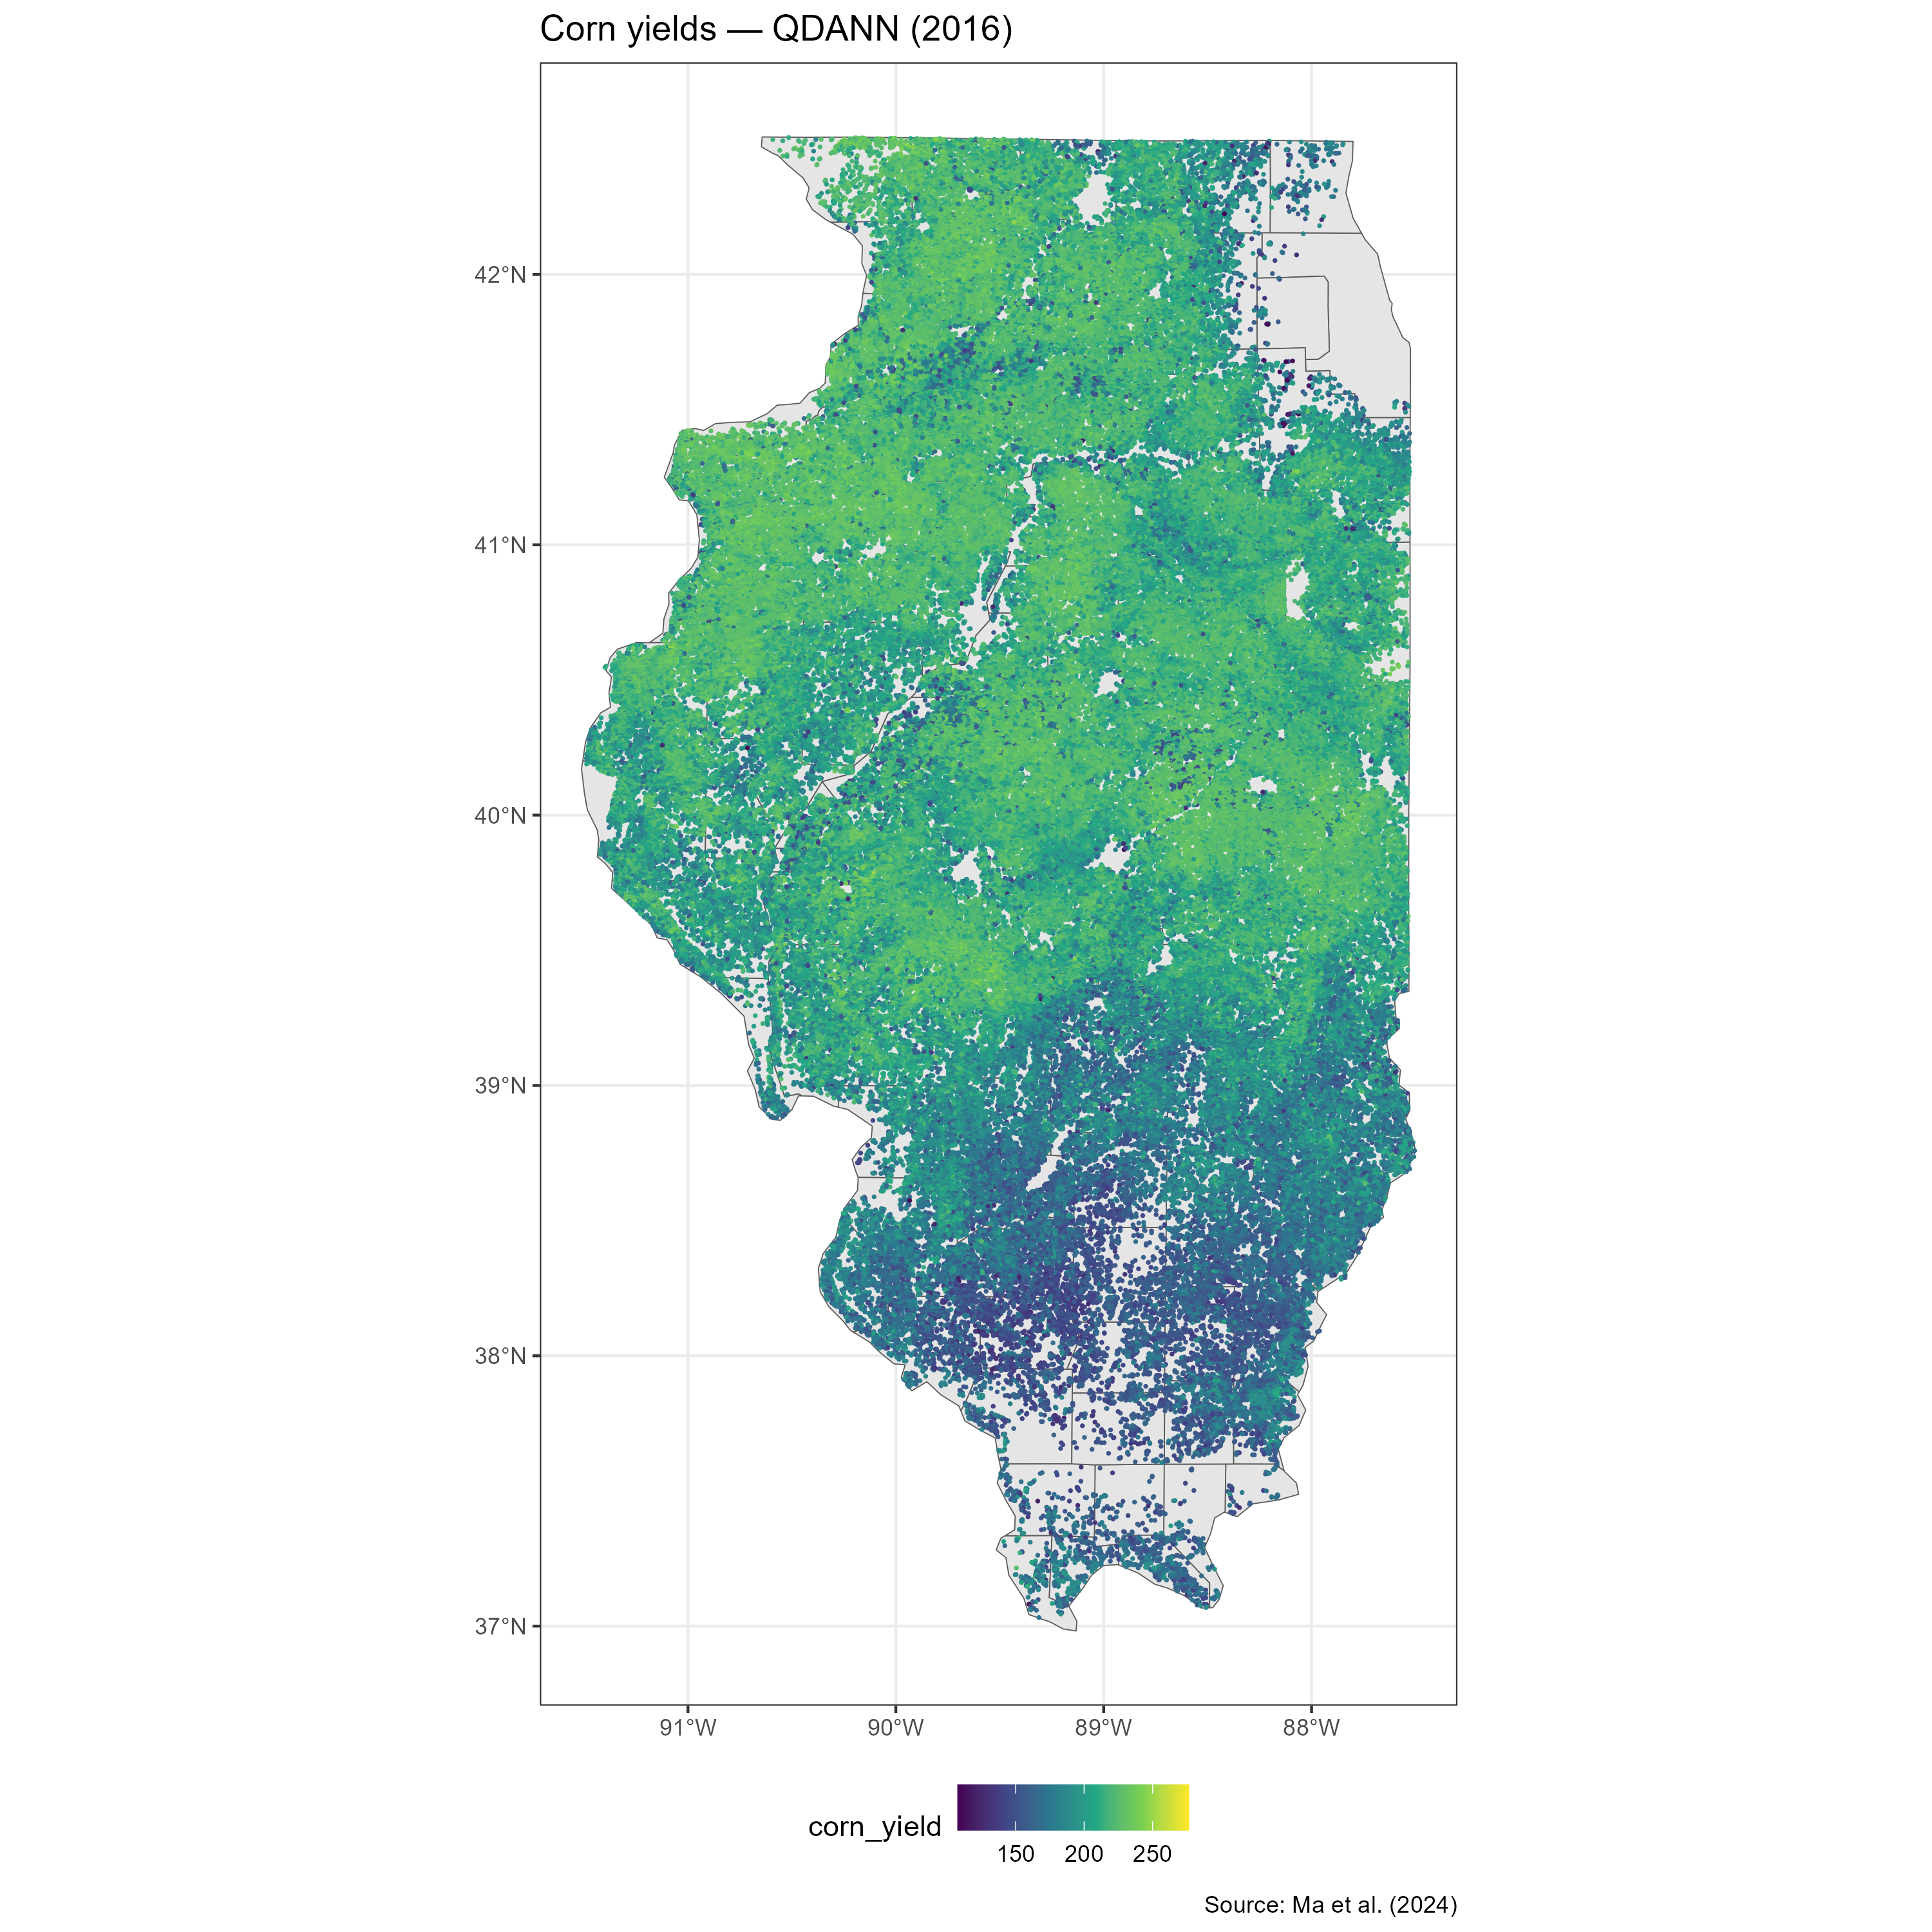
\includegraphics[width=0.85\textwidth]{figures/corn_yield_map}
  \caption{QDANN corn yields across Illinois, 2016.}
  \label{fig:corn_yield_map}
  \floatfoot{\footnotesize Notes: Spatial distribution of QDANN field-level corn
  yield estimates for Illinois in 2016. Source: \citet{Ma2024}.}
\end{figure}

\begin{figure}[H]
  \centering
  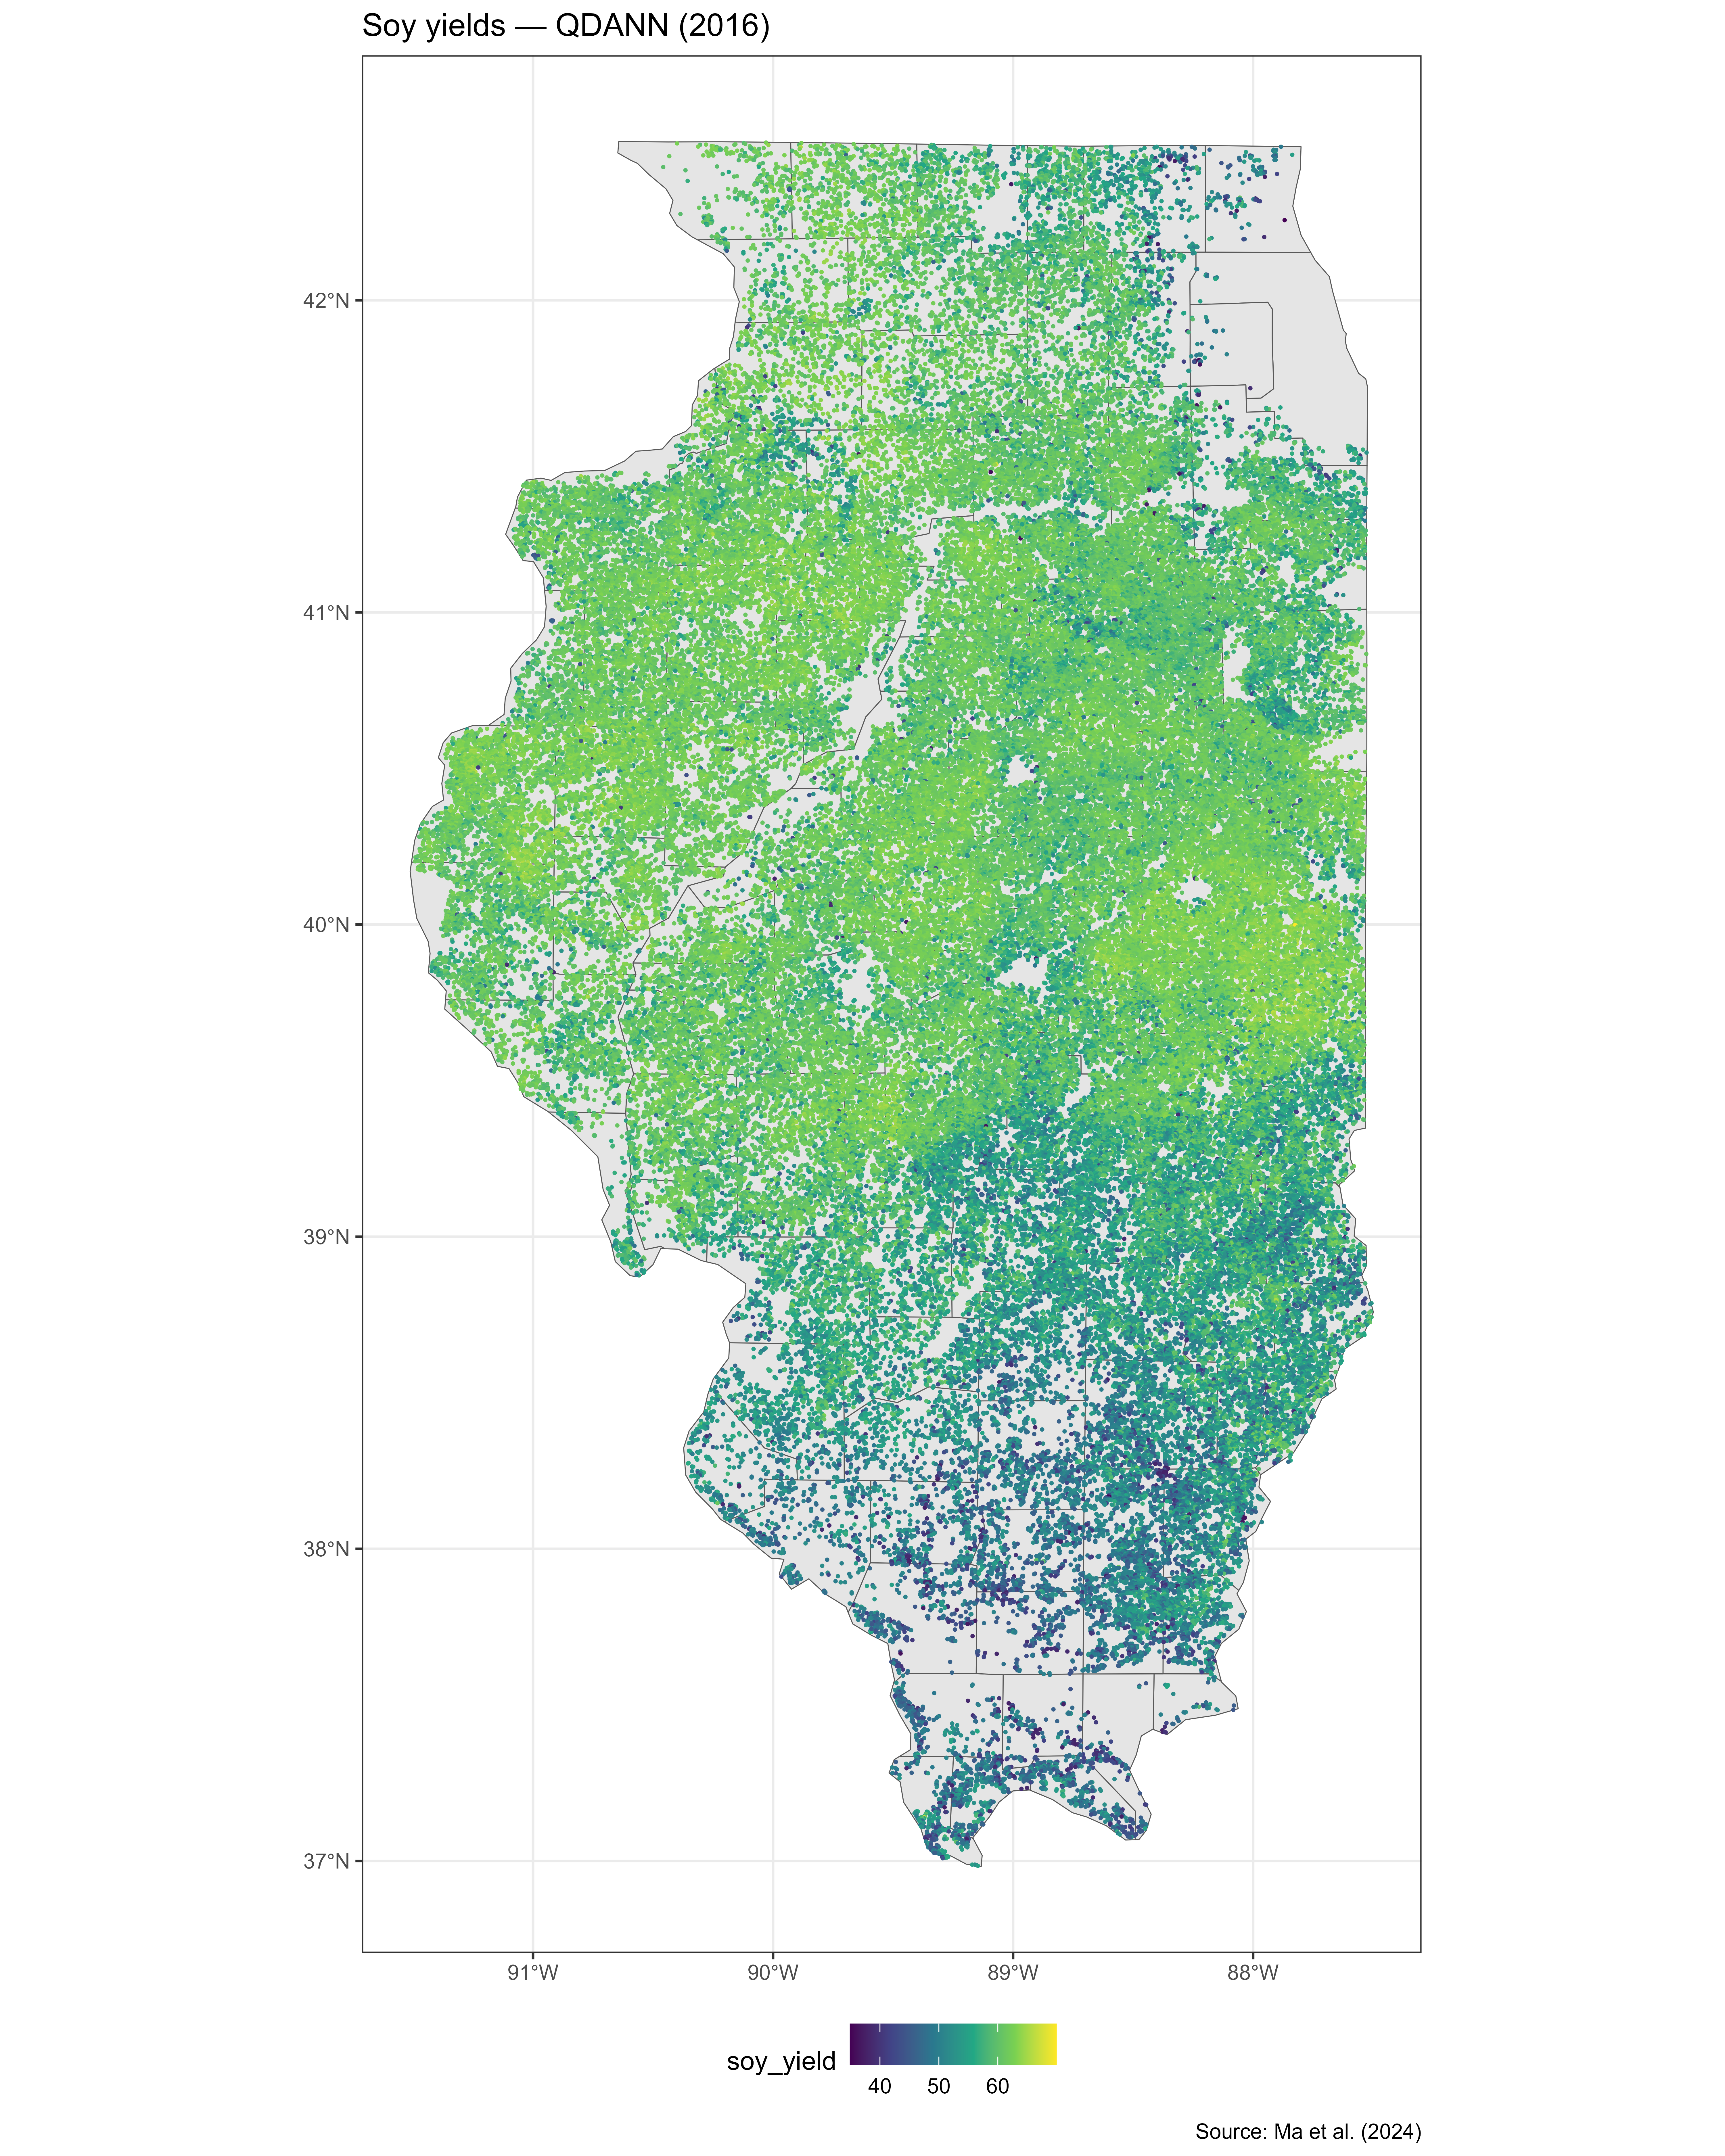
\includegraphics[width=0.85\textwidth]{figures/soy_yield_map}
  \caption{QDANN soybean yields across Illinois in 2016.}
  \label{fig:soy_yield_map}
  \floatfoot{\footnotesize Notes: Spatial distribution of QDANN field-level soybean
  yield estimates for Illinois in 2016. Source: \citet{Ma2024}.}
\end{figure}
 
\begin{figure}[H]
  \centering
  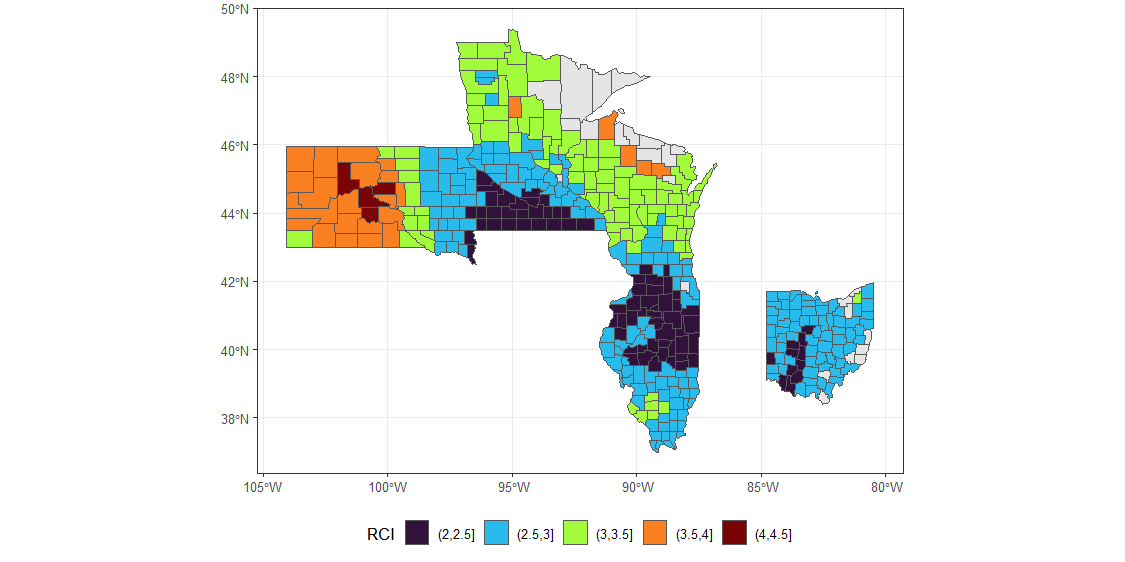
\includegraphics[width=0.85\textwidth]{figures/rci_map}
  \caption{Rotational Complexity Index across Illinois, 2016.}
  \label{fig:rci_map}
  \floatfoot{\footnotesize Notes: Spatial distribution of RCI values computed from
  six-year CDL crop histories at 30-meter resolution. Source: \citet{socolar2021};
  CDL data from USDA-NASS.}
\end{figure}

\subsection{\label{subsec:rot_seq}Crop History and Rotation Sequences}
Field-level crop histories come from the USDA Cropland Data Layer (CDL), an annual raster product produced by NASS that classifies each 30-meter pixel into a crop or land-cover category using satellite imagery and agricultural survey reference data. CDL has been available annually since 2008 for the full contiguous United States and since 2003 for Illinois. We use annual CDL data from 2003 to 2022 for Illinois, providing up to 20 years of rotation history for each field.

For each field-pixel and outcome year $t$, we construct a six-year rolling rotation sequence by recording the CDL-classified crop in each of years $t-1$ through $t-6$, classifying each year as corn (CDL code 1), soybean (CDL code 5), or other. We restrict the analysis to field-year observations satisfying three conditions: corn is the outcome crop in year $t$; the six-year history consists entirely of corn or soybean plantings with no years classified as other crops, fallow, or non-agricultural land cover; and the field appears in at least two consecutive years in the panel after singleton removal. The first two restrictions ensure that rotation sequences are clean binary strings over $\{corn, soybean\}$ and that the RCI and sequence indicators are well-defined. The third removes fields that appear in only one year and therefore contribute no identifying variation. After these restrictions, the estimation sample contains 1,548,319 field-year observations for QDANN and 1,411,846 for SCYM, the difference reflecting variation in the spatial coverage of the two estimators across Illinois counties.

We characterize rotation histories in two complementary ways. The first is the full sequence of crop codes over the six-year window, which yields $2^6 = 64$ distinct binary sequences, of which 32 end in corn and are included in the corn yield regressions. Corn monoculture (coded $C-C-C-C-C-C$) serves as the reference category. The second characterization uses the RCI of \citet{socolar2021}, described in Section~\ref{subsec:rci}.

\subsection{\label{subsec:w_controls}Weather Controls}
Monthly precipitation totals, vapor pressure deficit (VPD), and a soil moisture index are derived from GRIDMET \citep{abatzoglou2013}, which is available at a spatial resolution of approximately 4 kilometers. We aggregate each variable to monthly totals or means for June, July, and August. Following \citet{SchlenkerRoberts2009}, we replace monthly mean temperature with growing degree days (GDD) accumulated between 8\textdegree C and 29\textdegree C, and extreme degree days (EDD) accumulated above 29\textdegree C. Climate water deficit data come from TerraClimate \citep{abatzoglou2018}.

\subsection{\label{subsec:soil_controls}Soil Controls}
Soil characteristics come from gSSURGO, produced by the USDA Natural Resources Conservation Service at 30-meter resolution. We extract three field-level measures: the National Commodity Crop Productivity Index (NCCPI), root zone available water storage (AWC), and soil organic carbon stock (SOC) in the 0-100-centimeter depth zone. NCCPI and SOC are collinear with county fixed effects and are dropped from the preferred specification; AWC is retained. Figure~\ref{fig:nccpi_corn_map} shows the spatial distribution of NCCPI across Illinois.

\subsection{\label{subsec:smaple_const}Sample Construction and Summary Statistics}
The estimation sample is constructed by merging the QDANN and SCYM yield rasters with CDL rotation sequences, GRIDMET and TerraClimate weather covariates, and gSSURGO soil variables at the 30-meter pixel level. Final sample sizes are 1,548,319 field-year observations (QDANN) and 1,411,846 (SCYM).

%\begin{table}[H]
  %\centering
  %\caption{Summary statistics by rotation type}
  %\label{tab:summary}
  %\begin{threeparttable}
    \begin{table}[!h]
\centering
\caption{\label{tab:summary}Summary statistics by rotation type}
\centering
\resizebox{\ifdim\width>\linewidth\linewidth\else\width\fi}{!}{
\begin{tabular}[t]{lrrrrrrrr}
\toprule
Rotation type & N & Corn yield & RCI & Precip (Jun) & GDD (Jul) & EDD (Jul) & VPD (Jul) & AWC (mm)\\
\midrule
Corn monoculture & 154570 & 11749.9 (2083.2) & 0.61 (0.80) & 140.9 (70.2) & 409 (52) & 268.3 (2.8) & 1.19 (0.73) & 254 (46)\\
Perfect rotation & 894537 & 12428.8 (1756.4) & 2.18 (0.37) & 139.2 (65.7) & 418 (41) & 268.3 (2.0) & 0.99 (0.42) & 240 (45)\\
Transitioning & 242285 & 12098.4 (1949.6) & 1.78 (0.24) & 142.6 (66.3) & 408 (48) & 267.9 (2.3) & 1.02 (0.50) & 249 (45)\\
\bottomrule
\end{tabular}}
\end{table}

    \begin{minipage}{\textwidth}
      \footnotesize
      Notes: Means and standard deviations (in parentheses) for QDANN corn yields and key covariates, by rotation type.      
      Corn monoculture = C-C-C-C-C-C; Perfect rotation = alternating C-S sequence; Transitioning = sequences with RCI between 1.41 and 2.00.
    \end{minipage}
  %\end{threeparttable}
%\end{table}
	
\section{Econometric Framework\label{sec:econ_framework}}
\subsection{\label{subsec:just_pope}The Just-Pope Framework and Its Variants}
The stochastic production function literature offers several approaches to jointly estimating the effects of inputs and management practices on the mean and variance of output. We briefly review the main variants to situate our estimator relative to the existing literature and motivate the specific implementation choices made here.

\medskip\noindent\textbf{Original two-stage OLS/FGLS - \cite{Just1978, Just1979}}. 

Just and Pope proposed a general stochastic production specification of the form:

\begin{equation}
    y = f(\mathbf{X},\alpha)+\sqrt{h(\mathbf{X},\beta)}\times \varepsilon
\end{equation}

where $f(\cdot)$ is the conditional mean function and $h(\cdot)$ is the conditional variance function, both functions of the same input vector $\mathbf{X}$. This formulation relaxes the multiplicative stochastic restriction that dominated prior work - which
required inputs to be either uniformly risk-increasing or risk-neutral - and allows any input to independently raise or lower yield variance. From an econometric standpoint, the specification is a heteroskedastic regression model in which the variance of the production error is itself a function of inputs. The original estimation procedure uses two stages: OLS of the mean function to recover residuals, then OLS (or NLS for nonlinear mean functions) of the squared residuals on the variance function covariates.

\medskip\noindent\textbf{Antle's flexible moment-based extension - \cite{antle1983, Antle2010}}. 

\cite{antle1983} extended the Just-Pope framework to estimate higher moments of the output distribution beyond the mean and variance, showing that the first three moments of milk yield are statistically significant functions of inputs. This matters for
insurance applications because indemnities are driven by left-tail probabilities, and mean-variance summaries may miss important skewness effects. \cite{Antle2010} later proposed partial-moment functions as a flexible way to characterize asymmetric input effects on output distributions. We do not implement the Antle extension here, but note that estimating skewness effects of rotation sequences on corn yields is a natural extension of our analysis.

\medskip\noindent\textbf{Maximum likelihood and log-linear variance - \cite{Harvey1976, Saha1997}}. 

Just-Pope functions have traditionally been estimated using feasible generalized least squares (FGLS). \cite{Saha1997} use Monte Carlo experiments showing that, in small samples, even when the error distribution departs from normality, the maximum likelihood (ML) estimator is more efficient and less biased than FGLS, and that FGLS can seriously understate the risk effects of inputs. A related improvement is the log-linear variance specification proposed by \cite{Harvey1976}, which replaces the linear regression of $\hat{\varepsilon}^2$ on $\mathbf{X}$ with a regression of $\log \hat{\varepsilon}^2$ on $\mathbf{X}$, then exponentiates fitted values to obtain strictly positive variance estimates. This avoids the truncation problem that arises when the linear approximation produces negative fitted values for some cells. We implement the three-stage FGLS estimator with a linear variance specification and
address the truncation problem by flooring negative fitted values at a small positive constant (see Section 4.2); we report the log-linear specification as a robustness check.

\medskip\noindent\textbf{Joint estimation with risk preferences and technical efficiency - \cite{Kumbhakar2002}}.

\cite{Kumbhakar2002} embeds the Just-Pope variance function inside a stochastic frontier model, jointly estimating production risk, risk preferences, and technical inefficiency without imposing parametric restrictions on the utility function. A limitation of the standard Just-Pope formulation is that it does not account for producers'  preferences, so that input elasticities are treated as invariant to risk perceptions. Kumbhakar's extension addresses this at the cost of additional distributional assumptions on the inefficiency term. We do not pursue this extension here, as our primary interest is in the population distribution of rotation effects rather than in individual farm efficiency.

\medskip\noindent\textbf{Nonparametric extension - \cite{li2021}}. 

The most flexible variant in the recent literature is the nonparametric production risk estimator of \cite{li2021}, in which both the mean function $f(\cdot)$ and the variance function $h(\cdot)$ are estimated using local polynomial regression rather than parametric functional forms. This allows the risk effect of any variable to vary continuously with a conditioning covariate - for example, the variance effect of a recent soybean placement varying smoothly with soil productivity. The LRZ estimator nests the parametric Just-Pope model as a special case in which the local polynomial slopes are constant. We implement the parametric Just-Pope estimator as our main specification and the LRZ nonparametric extension as a robustness check, allowing rotation effects to vary with NCCPI soil productivity, following the approach described in Section 4 of \cite{li2021}.

Our main estimator follows the three-stage FGLS approach of \cite{Harvey1976} and \cite{Saha1997}, embedded in a panel fixed effects framework with two-way clustering for inference. The specific implementation is described in Sections 4.2 through 4.4 below.

\subsection{\label{subsec:stage_1}Conditional Mean: Stage 1}
We model the conditional mean of corn yields as a two-way fixed effects regression following the linear panel framework:

\begin{equation}
    y_{it}=\text{seq}_{it}'\tau+ W_{it}'\beta+\lambda_{k}+\gamma_{t}+\varepsilon_{it}\label{eq:stage1}
\end{equation}

where $y_{it}$ is the yield of field $i$ year $t$ measured in bushels per acre; $\text{seq}_{it}$ is either a vector of rotation sequence indicators (with corn monoculture as the reference category) or a vector of factor RCI indicators (with the lowest observed RCI as the reference); $W_{it}$ is a vector of weather and soil controls described in Section 3.3; $\lambda_{k}$ is a county (FIPS) fixed effect; and $\gamma_{t}$ is a year fixed effect. The error term $\varepsilon_{it}$ is assumed to
have mean zero conditional on the regressors.

County fixed effects absorb all time-invariant differences across counties in average yield levels - including persistent soil quality gradients, drainage infrastructure, and local agronomic practices. Year fixed effects absorb common shocks to all fields in a given year, including statewide weather events and aggregate commodity price signals that affect input use uniformly. Identification of the rotation effect $\hat{\tau}$ therefore comes from within-county, across-field variation in rotation sequences over time, conditional on the weather and soil controls. Standard errors are  clustered two-way at the field $\text{tile\_field\_ID}$) and year levels, following \cite{Cameron2015}, to account for both within-field serial correlation in the panel and cross-sectional dependence across fields in the same growing season driven by common weather shocks.

\medskip\noindent\textbf{Principal components analysis of rotation features}. To motivate the parsimonious Z-vector parameterization, we conduct a principal components analysis (PCA) of the RCI-level rotation feature space. igure~\ref{fig:rot_pca_plot} shows the biplot of the first two principal components across the 18 distinct RCI values in our Illinois corn-soy sample. PC1 explains 83.3 percent of the total variance, and PC2 explains 9.6 percent, so together they account for 93 percent of the total variance. The near-complete dimensionality reduction confirms that four well-chosen structural features suffice to characterize the rotation space.

\begin{figure}[H]
  \centering
  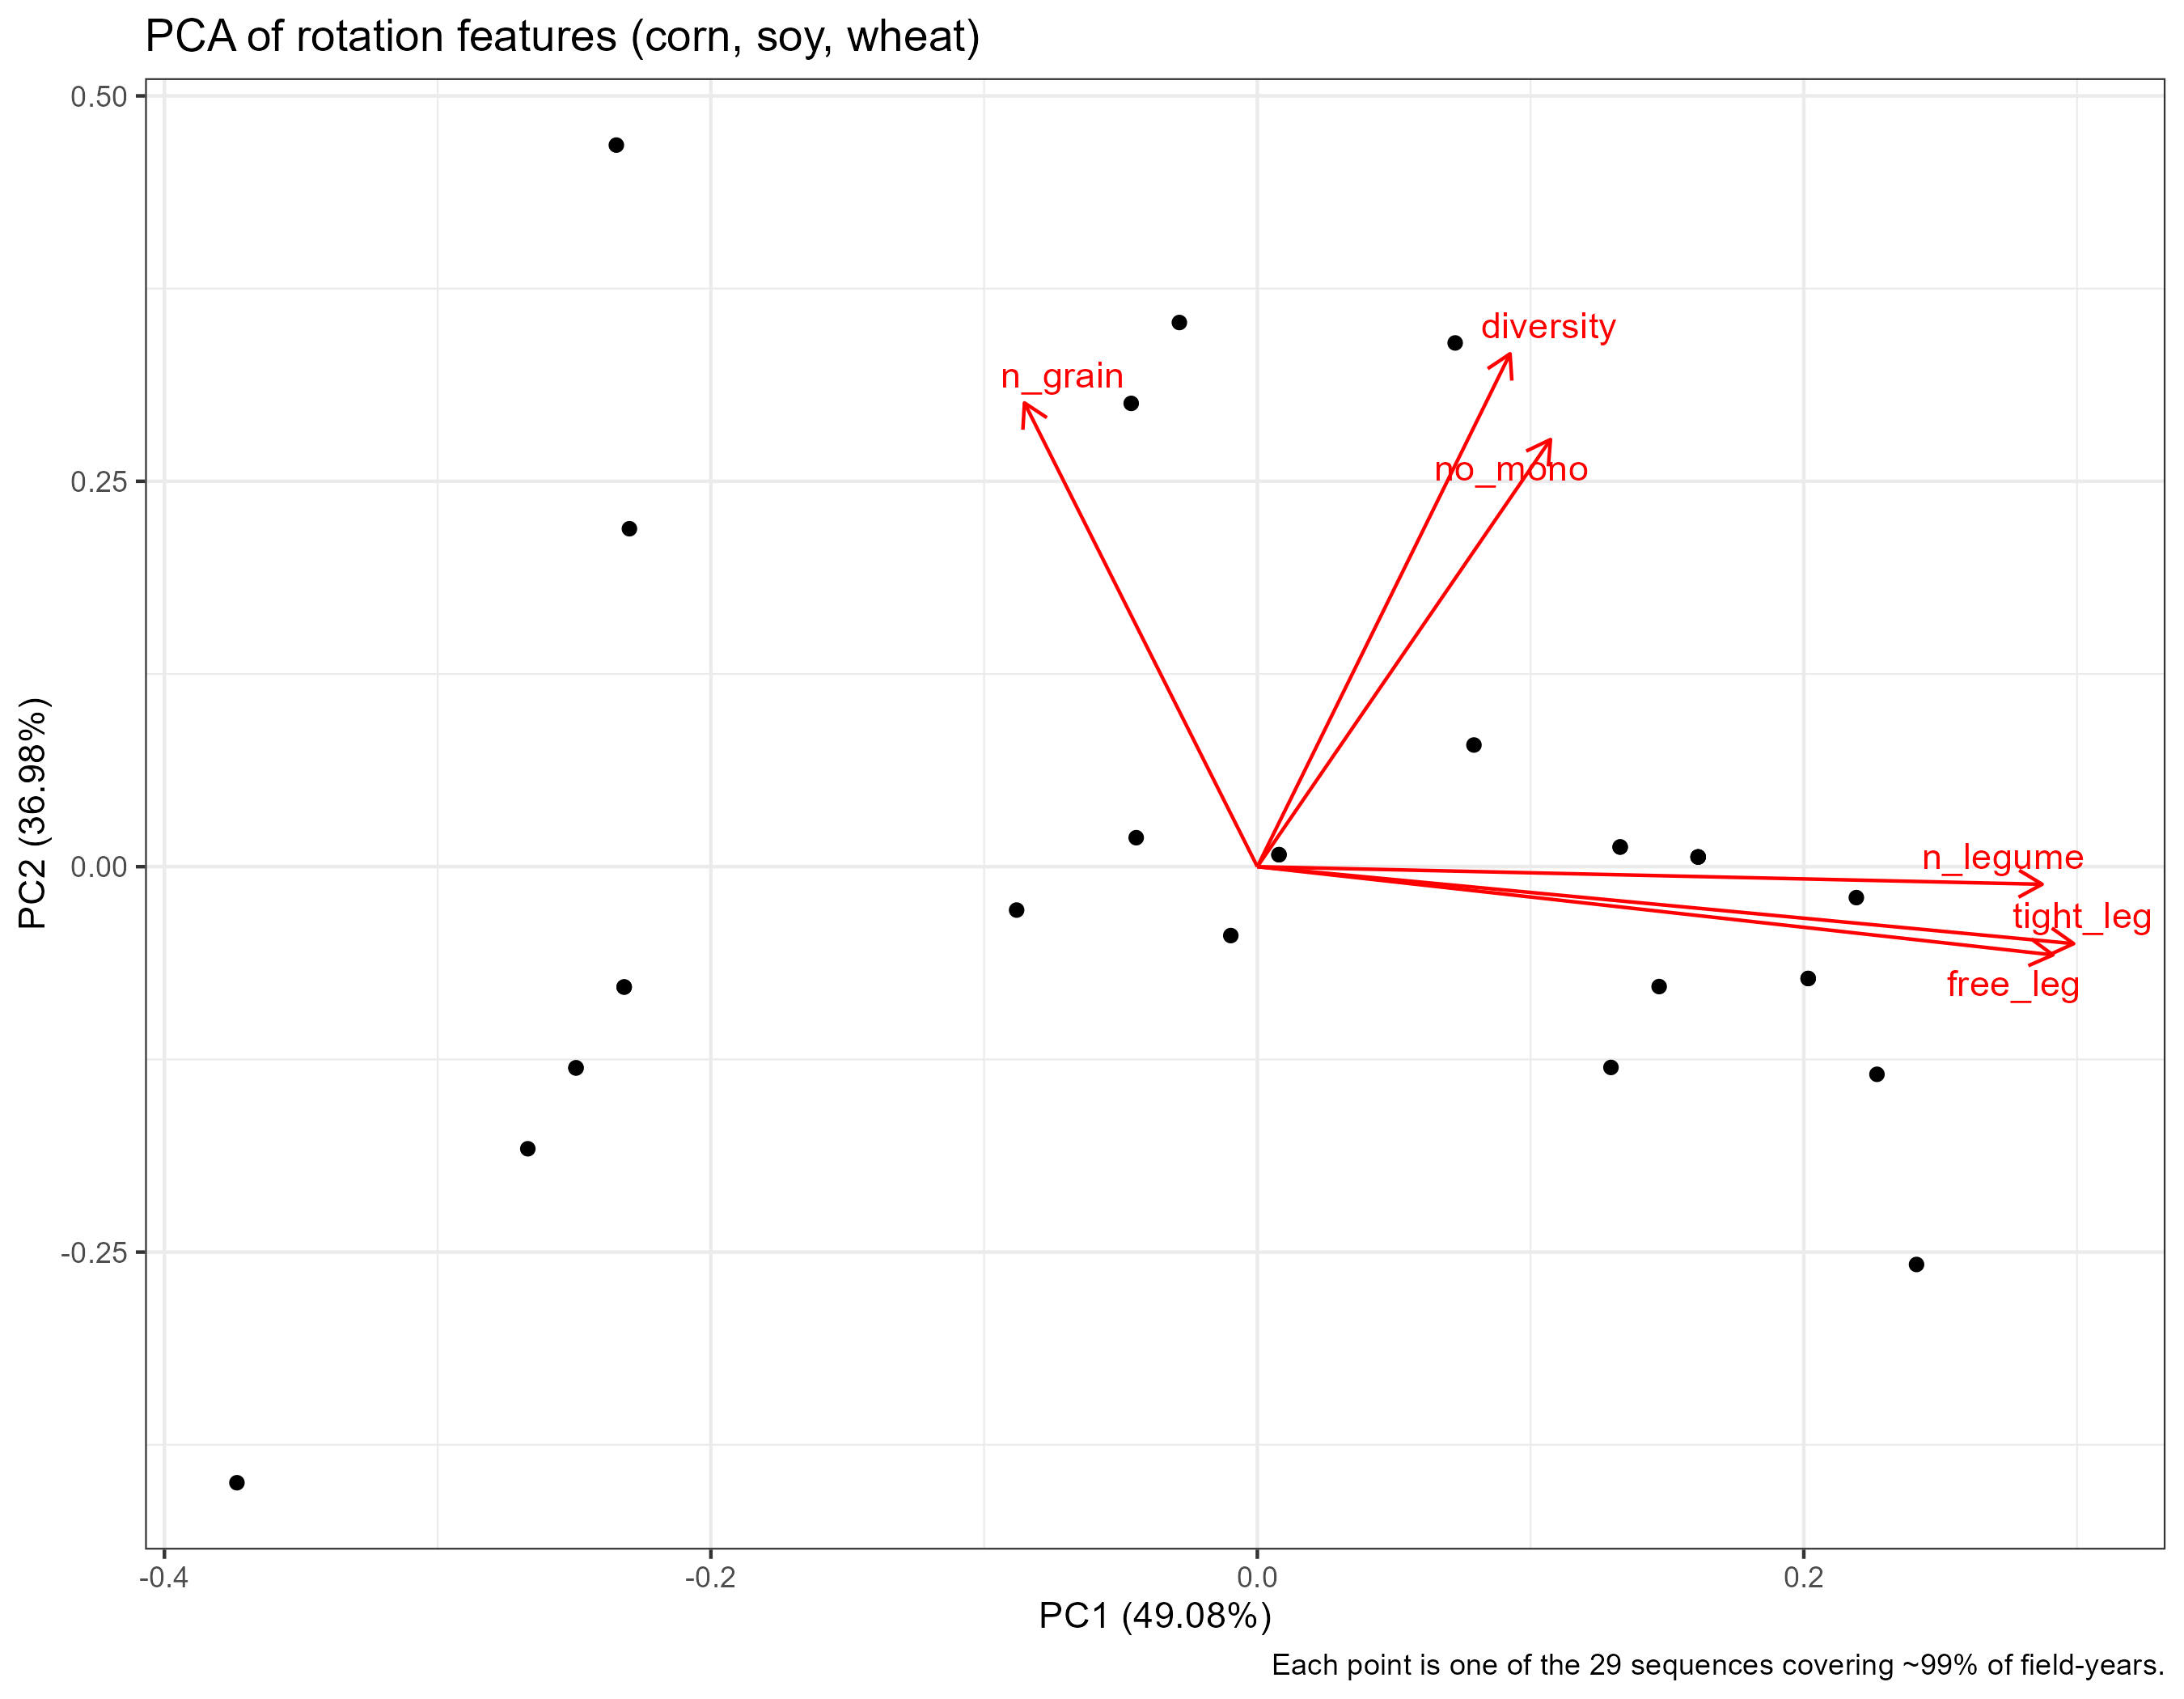
\includegraphics[width=0.75\textwidth]{figures/rot_pca_plot}
  \caption{PCA biplot of corn-soy rotation features.}
  \label{fig:rot_pca_plot}
  \floatfoot{\footnotesize Notes: Biplot of the first two principal components across the 18 distinct RCI values observed in the Illinois corn-soy sample. PC1 explains 83.3\% of the total variance, and PC2 explains 9.6\%. Red arrows show loadings of four rotation summary features: $n\_\text{soy}$, $\text{no\_consec}$, $\text{tight\_soy}$, and $\text{free\_soy}$.}
\end{figure}

We also estimate a parsimonious parameterization that replaces the sequence indicators with four structural rotation features:
%
\begin{equation}
  y_{it} = Z_{it}'\tau + W_{it}'\beta + \lambda_k + \gamma_t + \varepsilon_{it}
  \label{eq:zvector}
\end{equation}
%
 Where $Z_{it} = [\text{late\_soy}_{it},\ \text{soy\_cons}_{it},\ \text{soy\_gap}_{it},\text{nsoy}_{it}]$: the soy lag (periods since most recent soybean harvest), a consecutive-soy dummy, the minimum gap between soybean harvests, and the total number of soybean harvests in the window.
 
Because the 31 sequence indicators are tested simultaneously against the monoculture reference, we report \cite{Benjamini1995} false discovery rate-adjusted p-values alongside unadjusted p-values in Table~\ref{tab:corn_rot}. The parsimonious Z-vector model in Table~\ref{tab:zvector} is our confirmatory specification with four pre-specified hypotheses; the sequence-level results are treated as exploratory.

\subsection{\label{subsec:stage_2}Conditional Variance: Stage 2 (Just-Pope Framework)}

To separately identify the effect of rotations on yield risk, we follow \cite{Just1979} and \cite{antle1983} in estimating a second-stage regression of squared first-stage residuals on the same regressors. Let $\hat{u}_{it} = y_{it}-\hat{y}_{it}$ denote
the residual from the stage-1 conditional mean regression. The second moment is then estimated as:

\begin{equation}
    \hat{u}_{it}^2 = \text{seq}_{it}'\pi + W_{it}'\delta + \lambda_k + \gamma_t + \nu_{it}\label{eq:stage2}
\end{equation}

Coefficients $\hat{\pi}$ identify the differential effect of each rotation sequence on the conditional variance of yields, relative to the monoculture reference. A negative coefficient indicates that a given sequence compresses yield variance relative to monoculture - a risk-reducing effect directly relevant to insurance pricing. A positive coefficient indicates that the sequence raises variance, increasing actuarial risk at any given mean yield level.

The squared residual $\hat{u}_{it}^2$ is a noisy proxy for the true conditional variance, since it combines the variance signal with idiosyncratic estimation error from stage 1. To improve estimation efficiency, we implement a three-stage Feasible Generalized Least Squares (FGLS) estimator following \cite{Harvey1976}. In stage 2a, we estimate an initial OLS regression of $\hat{u}_{it}^2$ on the full set of covariates to obtain fitted values $\hat{h}_{it}$, which serve as estimates of the conditional variance function. In stage 2b, we re-estimate the variance regression by Weighted Least Squares (WLS), weighting each observation by $1/\hat{h}_{it}$ where $\hat{h}{it}= \max(\hat{h}_{it}^{\text{OLS}},\ \varepsilon)$ with $\varepsilon = 10^{-6}$ to prevent degenerate weights from negative linear approximations to the variance function. The FGLS estimator is more efficient than the OLS second-stage estimator because it downweights observations whose squared residuals are expected to be highly variable - those from rotation sequences with high estimated conditional variance.

\subsection{\label{subsec:bootstrap}Inference: Three-Stage Bootstrap}

Both the OLS and FGLS stage-2 estimators face a generated-regressor problem: the dependent variable $\hat{u}_{it}^2$ is constructed from first-stage estimates and therefore contains estimation error that standard second-stage standard errors do not account for. In the FGLS case, the weights $\hat{h}_{it}$ are themselves estimated, introducing a third source of uncertainty. We address the generated-regressor problem for both estimators by implementing a pairs cluster bootstrap that wraps all three stages, propagating first-stage uncertainty through to the final variance estimates.

The bootstrap procedure proceeds as follows. In each of $B = 999$ iterations, we draw a bootstrap sample by resampling $n$ fields with replacement from the $n$ unique fields in the estimation sample, where the bootstrap weight of field $j$ equals the number of times it was drawn. Rather than physically duplicating rows - which at approximately 1.55 million observations would exhaust available memory - we implement a frequency-weight bootstrap that assigns each field a bootstrap weight equal to its draw count and passes this weight to all three estimation stages via the \texttt{weights} argument of the regression function. Fields not drawn receive weight zero and are excluded from that iteration. Within each iteration, stages 1, 2a, and 2b are re-estimated on the weighted sample, and the stage-2b coefficient vector is stored. Bootstrap standard errors are computed as the standard deviation of the stored coefficient draws across $B$ iterations, and 95 percent confidence intervals are constructed as the 2.5th and 97.5th percentiles of the bootstrap distribution. All fixed effects and clustering are maintained within each bootstrap iteration.

This bootstrap design has two important properties. First, by resampling at the field level, it respects the within-field serial correlation in the panel - all years of a given field enter the bootstrap sample together or not at all. Second, by wrapping all
three stages in a single loop, the bootstrap correctly accounts for the covariance between the stage-1 residuals and the stage-2 weights, which a naive two-step bootstrap that treats stage-1 as fixed would miss.

\subsection{\label{subsec:rot_score}Rotation Score}
The four structural feature coefficients from the parsimonious stage-1 model admit a natural rotation scoring rule. For each field-year observation, we define the rotation score as:

\begin{equation}
    \text{score}_{it} = \hat{\tau}_1 \cdot \text{late\_soy}_{it} + \hat{\tau}_2 \cdot \text{soy\_cons}_{it} + \hat{\tau}_3 \cdot \text{soy\_gap}_{it} + \hat{\tau}_4 \cdot n\text{soy}_{it}\label{eq:score}
\end{equation}

where $\hat{\tau}_1, \ldots, \hat{\tau}_4$ are the QDANN stage-1 estimates from Table 1. The score summarizes, in units of predicted yield deviation from monoculture, the information contained in the six-year rotation history relevant to the conditional mean of corn yields. By construction, corn monoculture - which has no soybean years in the window - scores zero. The perfect alternating corn-soybean rotation yields approximately 2.59 bushels per acre more than monoculture under the QDANN specification.

Rotation sequences that score below zero have structural features that are predicted to lower mean yields relative to continuous corn; these sequences typically involve multiple consecutive soybean years or very infrequent soybean harvests that deplete
the nitrogen and pest-suppression benefits of rotation. Sequences that score above zero have structural features associated with higher mean yields, particularly a recent soybean harvest and adequate spacing between soybean years.

%The rotation score maps all 64 binary six-year corn-soy sequences onto [$K$] distinct score values, providing a parsimonious and interpretable basis for rating that collapses the combinatorial rotation space into a single actuarial variable. In Section 5.3 we
%show that score-based yield predictions recover most of the variation captured by the full sequence-indicator model, and in Section 6 we discuss how the score could be incorporated into APH-based rate adjustments.

\section{\label{sec:results}Results}
\subsection{\label{subsec:seq_effects}Sequence-Level Effects on Corn Yield Mean}
 
Table~\ref{tab:corn_rot} and Figure~\ref{fig:corn_rot_plot} report the estimated effects of each of the 31 non-monoculture six-year corn-soy sequences on the mean corn yield, relative to corn monoculture. Rotation effects are heterogeneous and depend critically on the recent history of soybean placement rather than on the total number of soybean years in the window.


\begin{table}[H]
   \caption{\label{tab:corn_rot} Rotation patterns and corn yields}
   \bigskip
   \centering
   \scriptsize
   \renewcommand*{\arraystretch}{0.8}
   \begin{tabular}{lcc}
      \toprule
       & \multicolumn{2}{c}{corn\_yield}\\
                                      & No controls              & With controls \\   
                                      & (1)                      & (2)\\  
      \midrule 
      W-C-C-S-W-C                     & 8.329$^{***}$ (1.537) [p<0.001]    & 7.630$^{***}$ (1.496) [p<0.001]\\   
      C-S-C-W-S-C                     & 8.170$^{***}$ (1.492) [p<0.001]    & 6.311$^{***}$ (1.368) [p<0.001]\\   
      S-S-C-S-S-C                     & 6.861$^{***}$ (0.5615) [p<0.001]   & 5.938$^{***}$ (0.5157) [p<0.001]\\   
      C-C-C-S-W-C                     & 6.826$^{***}$ (0.6815) [p<0.001]   & 5.810$^{***}$ (0.6512) [p<0.001]\\   
      S-C-S-W-S-C                     & 6.292$^{***}$ (0.6945) [p<0.001]   & 5.772$^{***}$ (0.6868) [p<0.001]\\   
      C-S-C-S-S-C                     & 5.430$^{***}$ (0.4847) [p<0.001]   & 4.824$^{***}$ (0.4312) [p<0.001]\\   
      S-S-S-S-S-C                     & 5.061$^{***}$ (0.6902) [p<0.001]   & 4.655$^{***}$ (0.5542) [p<0.001]\\   
      S-C-S-S-S-C                     & 5.270$^{***}$ (0.5453) [p<0.001]   & 4.609$^{***}$ (0.4616) [p<0.001]\\   
      C-C-C-C-S-C                     & 4.628$^{***}$ (0.3541) [p<0.001]   & 4.411$^{***}$ (0.3639) [p<0.001]\\   
      S-S-C-C-S-C                     & 5.004$^{***}$ (0.5438) [p<0.001]   & 4.308$^{***}$ (0.5122) [p<0.001]\\   
      C-S-S-S-S-C                     & 4.305$^{***}$ (0.6044) [p<0.001]   & 4.284$^{***}$ (0.5434) [p<0.001]\\   
      S-C-C-C-S-C                     & 4.696$^{***}$ (0.3683) [p<0.001]   & 4.230$^{***}$ (0.3499) [p<0.001]\\   
      S-C-C-S-W-C                     & 5.012$^{***}$ (0.7216) [p<0.001]   & 4.121$^{***}$ (0.6876) [p<0.001]\\   
      C-S-C-C-S-C                     & 4.494$^{***}$ (0.3984) [p<0.001]   & 4.089$^{***}$ (0.3658) [p<0.001]\\   
      C-C-S-C-S-C                     & 4.286$^{***}$ (0.4121) [p<0.001]   & 4.071$^{***}$ (0.3928) [p<0.001]\\   
      C-C-C-S-S-C                     & 3.602$^{***}$ (0.5559) [p<0.001]   & 3.746$^{***}$ (0.5121) [p<0.001]\\   
      S-C-S-C-S-C                     & 4.195$^{***}$ (0.4310) [p<0.001]   & 3.632$^{***}$ (0.3953) [p<0.001]\\   
      S-C-C-S-S-C                     & 3.943$^{***}$ (0.6356) [p<0.001]   & 3.287$^{***}$ (0.5725) [p<0.001]\\   
      S-S-S-C-S-C                     & 3.650$^{***}$ (0.5843) [p<0.001]   & 3.250$^{***}$ (0.5012) [p<0.001]\\   
      C-C-C-S-C-C                     & 2.463$^{***}$ (0.2341) [p<0.001]   & 2.105$^{***}$ (0.2482) [p<0.001]\\   
      C-S-C-S-C-C                     & 1.436$^{***}$ (0.3704) [p<0.001]   & 1.028$^{***}$ (0.3617) [p=0.005]\\   
      S-C-S-S-C-C                     & 1.214$^{**}$ (0.5779) [p=0.038]    & 0.6850 (0.5368) [p=0.205]\\   
      C-C-S-C-C-C                     & 0.9810$^{***}$ (0.2932) [p=0.001]  & 0.6844$^{**}$ (0.2820) [p=0.017]\\   
      S-C-S-C-C-C                     & 0.9022$^{***}$ (0.3191) [p=0.006]  & 0.4936 (0.3144) [p=0.119]\\   
      S-S-C-S-C-C                     & 0.0523 (0.6005) [p=0.931]          & -0.6638 (0.5569) [p=0.236]\\   
      C-S-C-C-C-C                     & -0.6166$^{**}$ (0.2826) [p=0.031]  & -0.7695$^{***}$ (0.2520) [p=0.003]\\   
      S-C-C-C-C-C                     & -0.7831$^{***}$ (0.2424) [p=0.002] & -1.076$^{***}$ (0.2311) [p<0.001]\\   
      S-S-C-C-C-C                     & -1.096 (0.7090) [p=0.125]          & -1.326$^{**}$ (0.6373) [p=0.040]\\   
       \\
      Observations                    & 1,796,806                & 1,796,806\\  
      R$^2$                           & 0.81623                  & 0.84354\\  
      Within R$^2$                    & 0.00690                  & 0.15452\\  
      Controls                        & No                       & Yes\\  
       \\
      tile\_field\_ID fixed effects   & $\checkmark$             & $\checkmark$\\   
      year fixed effects              & $\checkmark$             & $\checkmark$\\   
      \bottomrule
   \end{tabular}
\end{table}



\begin{quote}
\footnotesize
Notes: Dependent variable is QDANN corn yield in bushels per acre. Reference category: corn monoculture (C-C-C-C-C-C). Column (1) excludes weather and soil controls; column (2) includes full control vector. County and year fixed effects included throughout. Stars indicate BH-FDR adjusted significance: $^{***}$FDR$<$0.01, $^{**}$FDR$<$0.05, $^{*}$FDR$<$0.10.
\end{quote}


% NOTE: the outer \begin{table}[H]...\begin{threeparttable}...\end{threeparttable}...\end{table} wrapper that previously surrounded this \input has been removed. tables/corn_rot.tex already supplies its own \begin{table}...\caption{\label{tab:corn_rot}}...\end{table}; wrapping it in another table/threeparttable environment nests a float inside a float (and threeparttable inside internal vertical mode), which will not compile. This same fix is applied to every other \input{tables/*.tex} call in the Results and Appendix below. See the already-correct pattern for tables/summary_stats.tex earlier in the file, which avoids this by commenting out its outer wrapper.

\begin{figure}[H]
  \centering
  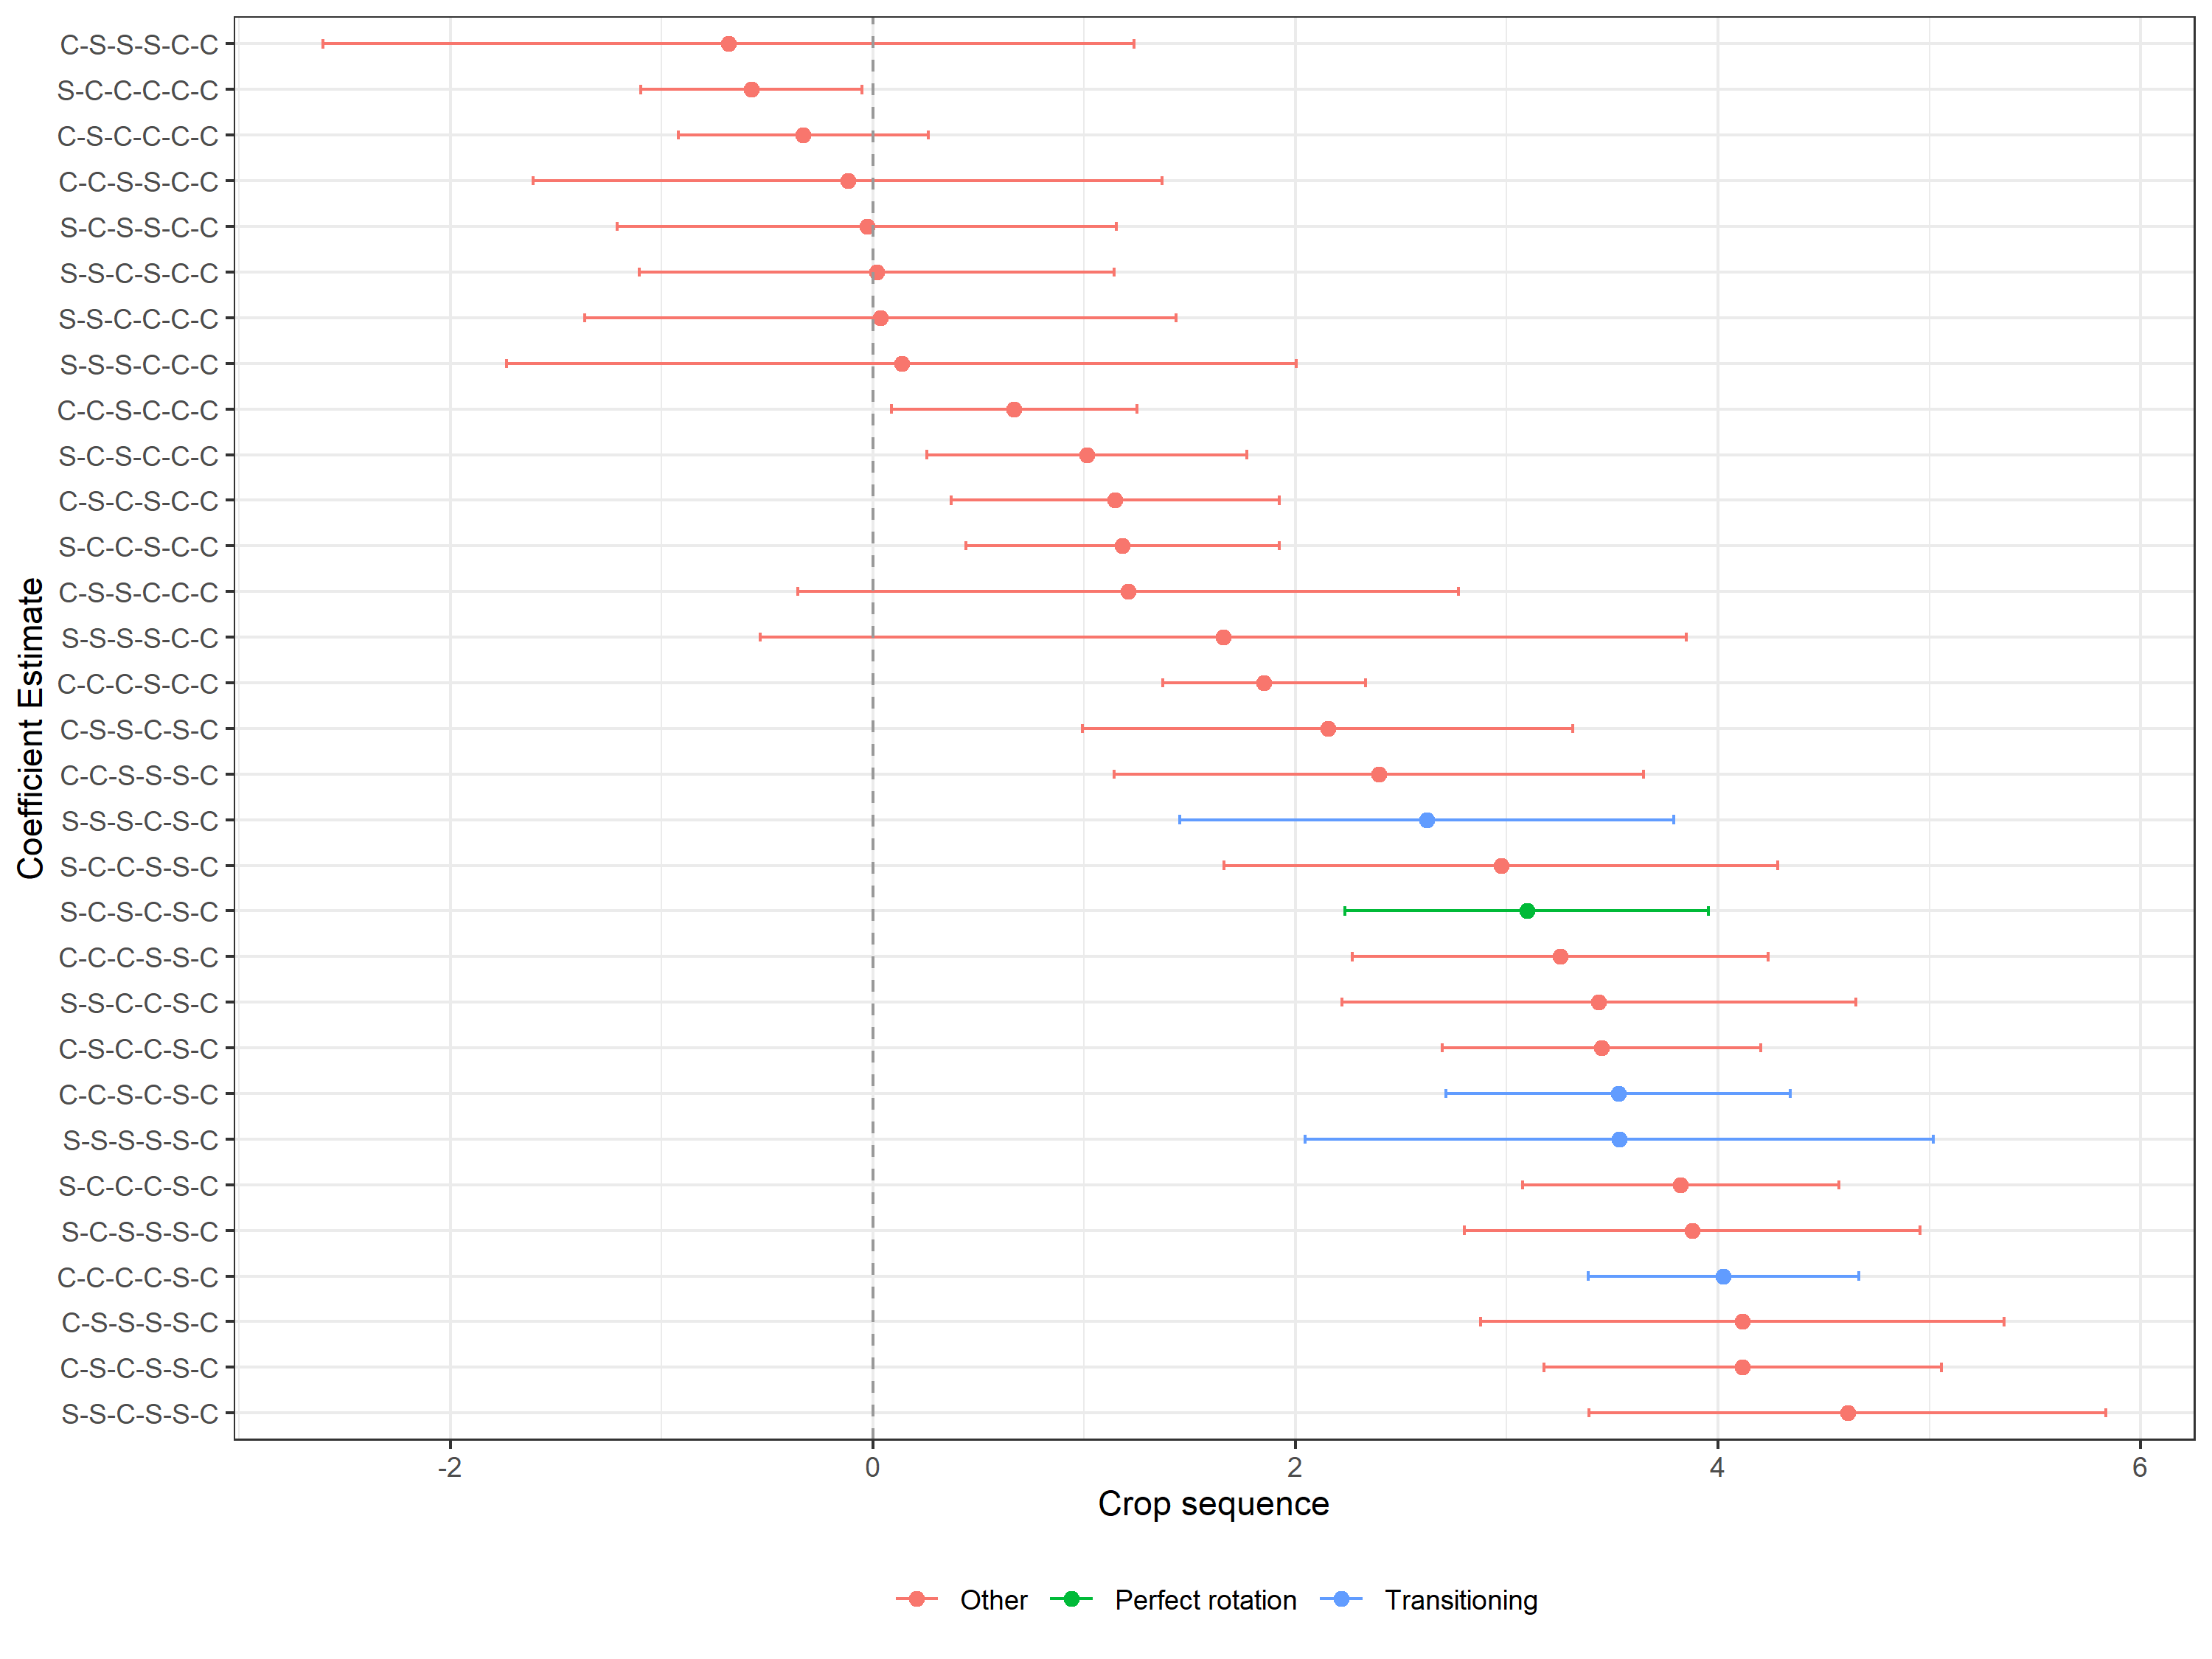
\includegraphics[width=0.90\textwidth]{figures/corn_rot_plot}
  \caption{Response of corn yields to rotation sequences.}
  \label{fig:corn_rot_plot}
  \floatfoot{\footnotesize Notes: Point estimates and 95\% confidence intervals from equation~\eqref{eq:stage1} with full controls. Reference: corn monoculture ($C-C-C-C-C-C$). Two-way clustering at field and year level. Green: perfect alternating rotation; blue: transitioning sequences; red: all others.}
\end{figure}
 
 
The highest-performing sequences in the QDANN specification-those with estimated mean yield premiums exceeding 4 bushels per acre-share a common structural feature: a soybean harvest in year $t-1$ or $t-2$, regardless of what was planted in years $t-3$ through $t-6$. For example, $S-S-C-S-S-C$ carries an estimated premium of 4.61 bushels per acre relative to monoculture (Table~\ref{tab:corn_rot}, column 2), and $S-C-S-C-S-C$ carries 4.12 bushels per acre. Both SCYM and QDANN yield consistent rankings at the top of the distribution.
% TODO: verify against tables/corn_rot.tex -- the current column-2 ("With controls") values are S-S-C-S-S-C = 4.799 and S-C-S-C-S-C = 2.896, not 4.61 and 4.12 as stated. Note S-C-S-C-S-C at 2.896 is still significant at the 1% level, so it may not belong in the ">4 bushels" group used to introduce this sentence; consider a different example sequence, or update the two figures cited.

Sequences ending in two or more consecutive corn years generally show negative or near-zero coefficients. The sequence $C-S-C-C-C-C$ has an estimated coefficient of $-0.58$ bushels per acre and is the only sequence with a statistically significant negative effect in the full specification. The perfect alternating corn-soybean rotation ($S-C-S-C-S-C$) carries a positive but statistically insignificant coefficient of approximately 2.45 bushels per acre: the rotation benefit materializes primarily through the most recent soybean placement rather than through a long-term rotation pattern.
% TODO: verify against tables/corn_rot.tex -- in the current table, C-S-C-C-C-C is -0.3703 and NOT significant, while a different sequence, S-C-C-C-C-C, is -0.5824 and significant at the 5% level ($^{**}$). The sequence names may have been transposed. Separately, S-C-S-C-S-C (used here for "the perfect alternating rotation") is listed at 2.896 with $p<0.01$ in column 2, which is both a different value and a different significance level than the "approximately 2.45... statistically insignificant" claimed here -- this also conflicts with the 4.12/significant framing implied two paragraphs above for the same sequence.
 
\subsection{\label{subsec:var_effects}Sequence-Level Effects on Corn Yield Variance}
 
Figure~\ref{fig:corn_var_plot} and the variance results in Table~\ref{tab:corn_jp_var} show the corresponding effects on the conditional variance of corn yields. Sequences that raise mean yields also tend to reduce yield variance, implying joint mean-variance dominance over monoculture. The most notable discrepancy between SCYM and QDANN is for sequences with a very recent soybean placement (year $t-1$): QDANN estimates a significant variance reduction of approximately 9 bushels-squared per acre-squared, while the SCYM estimate is positive and insignificant. This likely reflects SCYM's limited ability to characterize yield tails compared with QDANN's quantile-based training objective. Figure~\ref{fig:corn_jp_plot} summarizes the joint mean-variance results in a single scatter plot.


\begin{table}[H]
   \caption{\label{tab:corn_jp_var} Stage 2 --- Corn yield conditional variance (FGLS, bootstrap SE)}
   \bigskip
   \centering
   \begin{tabular}{lc}
      \toprule
                                       & resid\_sq\\   
                                       & (1)\\  
      \midrule 
      C-C-C-C-S-C                      & -2.608$^{*}$ (1.561)\\   
      C-C-C-S-C-C                      & -1.166 (1.888)\\   
      C-C-C-S-S-C                      & -3.954 (6.955)\\   
      C-C-C-S-W-C                      & -4.563 (7.625)\\   
      C-C-S-C-C-C                      & -2.51 ( 1.96)\\   
      C-C-S-C-S-C                      & -2.699$^{*}$ (1.543)\\   
      C-S-C-C-C-C                      & -0.9526 (1.995)\\   
      C-S-C-C-S-C                      & -1.582 (1.604)\\   
      C-S-C-S-C-C                      & -2.645 (  1.8)\\   
      C-S-C-S-S-C                      & -0.4388 (  2.1)\\   
      C-S-C-W-S-C                      & -6.375 (16.24)\\   
      C-S-S-S-S-C                      & 1.889 (7.323)\\   
      S-C-C-C-C-C                      & -2.932 ( 1.92)\\   
      S-C-C-C-S-C                      & -1.481 (1.712)\\   
      S-C-C-S-S-C                      & -4.991 (4.073)\\   
      S-C-C-S-W-C                      & -1.404 (9.155)\\   
      S-C-S-C-C-C                      & -0.6575 (1.899)\\   
      S-C-S-C-S-C                      & -2.12 (1.449)\\   
      S-C-S-S-C-C                      & 4.738 (5.055)\\   
      S-C-S-S-S-C                      & -1.519 (3.024)\\   
      S-C-S-W-S-C                      & -4.754 (5.753)\\   
      S-S-C-C-C-C                      & 12.53 (9.702)\\   
      S-S-C-C-S-C                      & -2.046 (4.119)\\   
      S-S-C-S-C-C                      & -3.69 (6.543)\\   
      S-S-C-S-S-C                      & 0.3054 (3.665)\\   
      S-S-S-C-S-C                      & -0.07085 ( 3.02)\\   
      S-S-S-S-S-C                      & -6.46 (4.635)\\   
      W-C-C-S-W-C                      & 16.42 ( 21.8)\\   
       \\
      Observations                     & 1,785,861\\  
      R$^2$                            & 0.60737\\  
      Within R$^2$                     & 0.00403\\  
       \\
      tile\_field\_ID fixed effects  & $\checkmark$\\   
      year fixed effects               & $\checkmark$\\   
      \bottomrule
   \end{tabular}
\end{table}



\begin{quote}
\small
Notes: Dependent variable is squared first-stage residual from the corn yield mean regression. OLS estimates of stage-2 variance equation~\eqref{eq:stage2}. Reference: corn monoculture. County and year fixed effects included. Two-way clustering at field and year level.
\end{quote}

\begin{figure}[H]
  \centering
  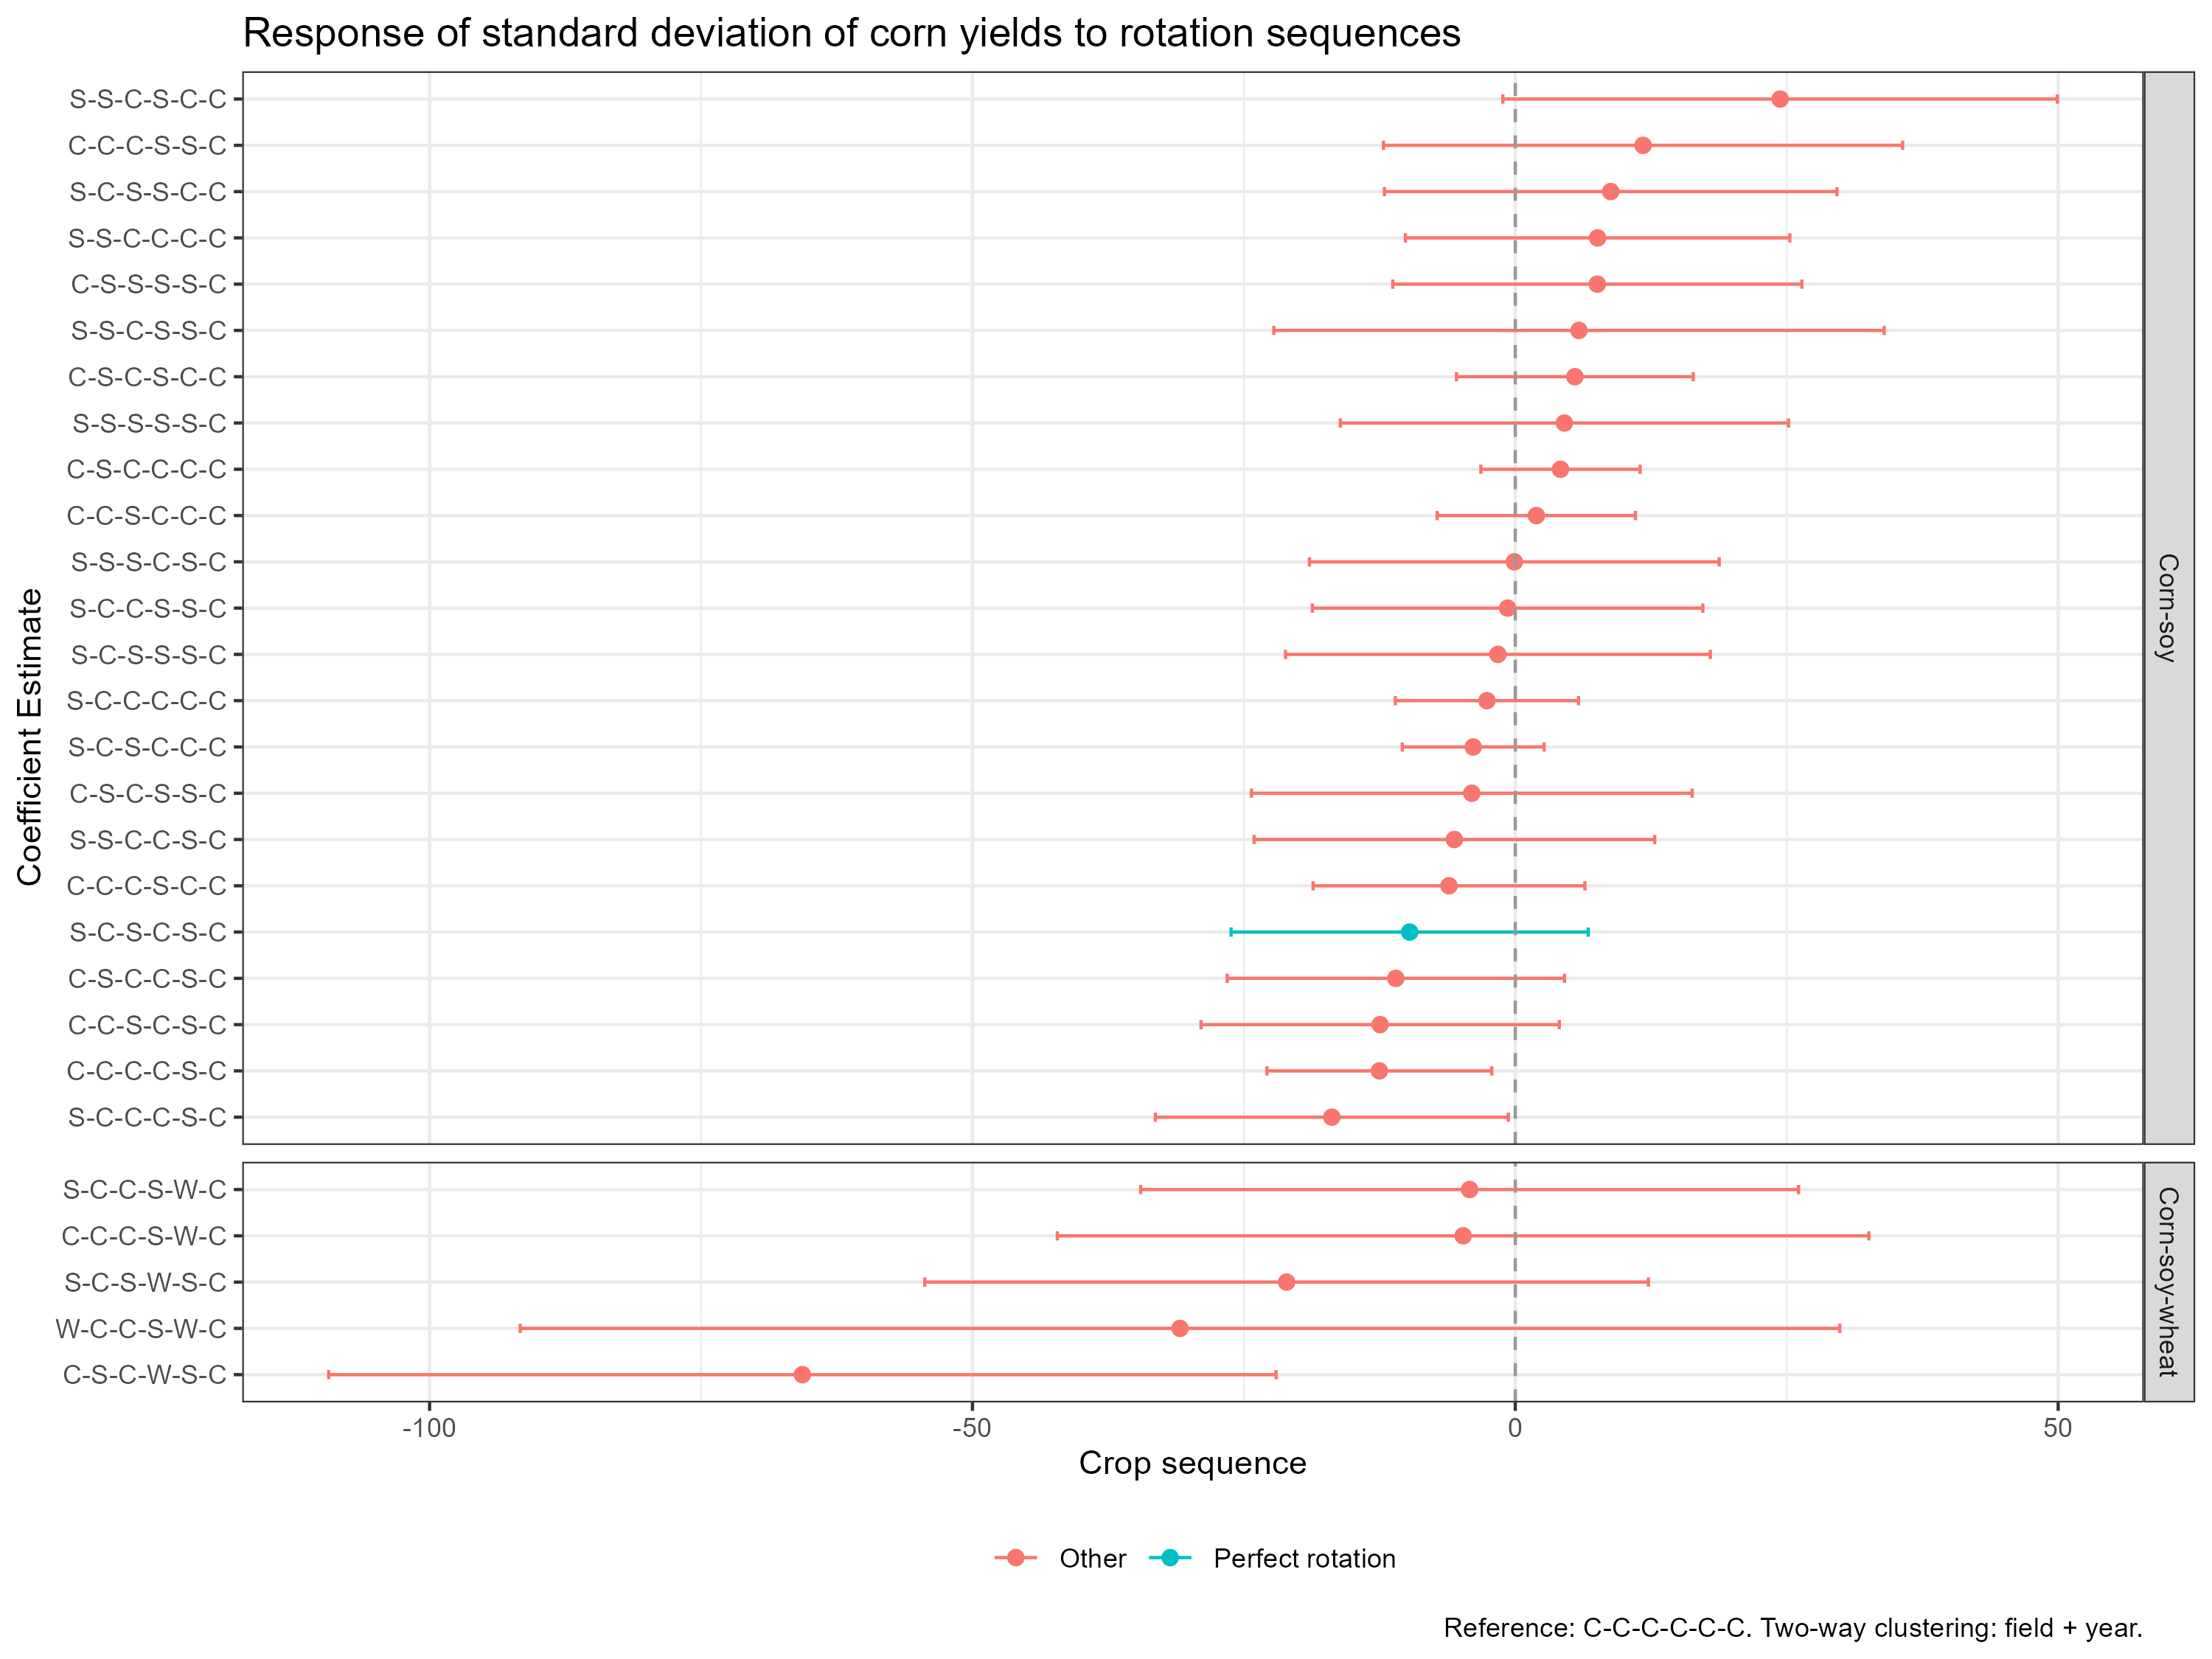
\includegraphics[width=0.90\textwidth]{figures/corn_var_plot}
  \caption{Response of the standard deviation of corn yields to rotation sequences.}
  \label{fig:corn_var_plot}
  \floatfoot{\footnotesize Notes: Point estimates and 95\% confidence intervals
  from stage-2 OLS variance regression. Reference: corn monoculture. Two-way
  clustering at field and year level.}
\end{figure}

Sequences that raise mean yields also tend to reduce yield variance, implying joint mean-variance dominance over monoculture. The most notable discrepancy between SCYM and QDANN is for sequences with a very recent soybean placement (year $t-1$): QDANN estimates a significant variance reduction of approximately 9 bushels-squared per acre-squared, while the SCYM estimate is positive and insignificant. This likely reflects SCYM's lower ability to characterize yield tails relative to QDANN's quantile-based training objective. Figure~\ref{fig:corn_jp_plot} summarizes the joint mean-variance results in a single scatter plot.

\begin{figure}[H]
  \centering
  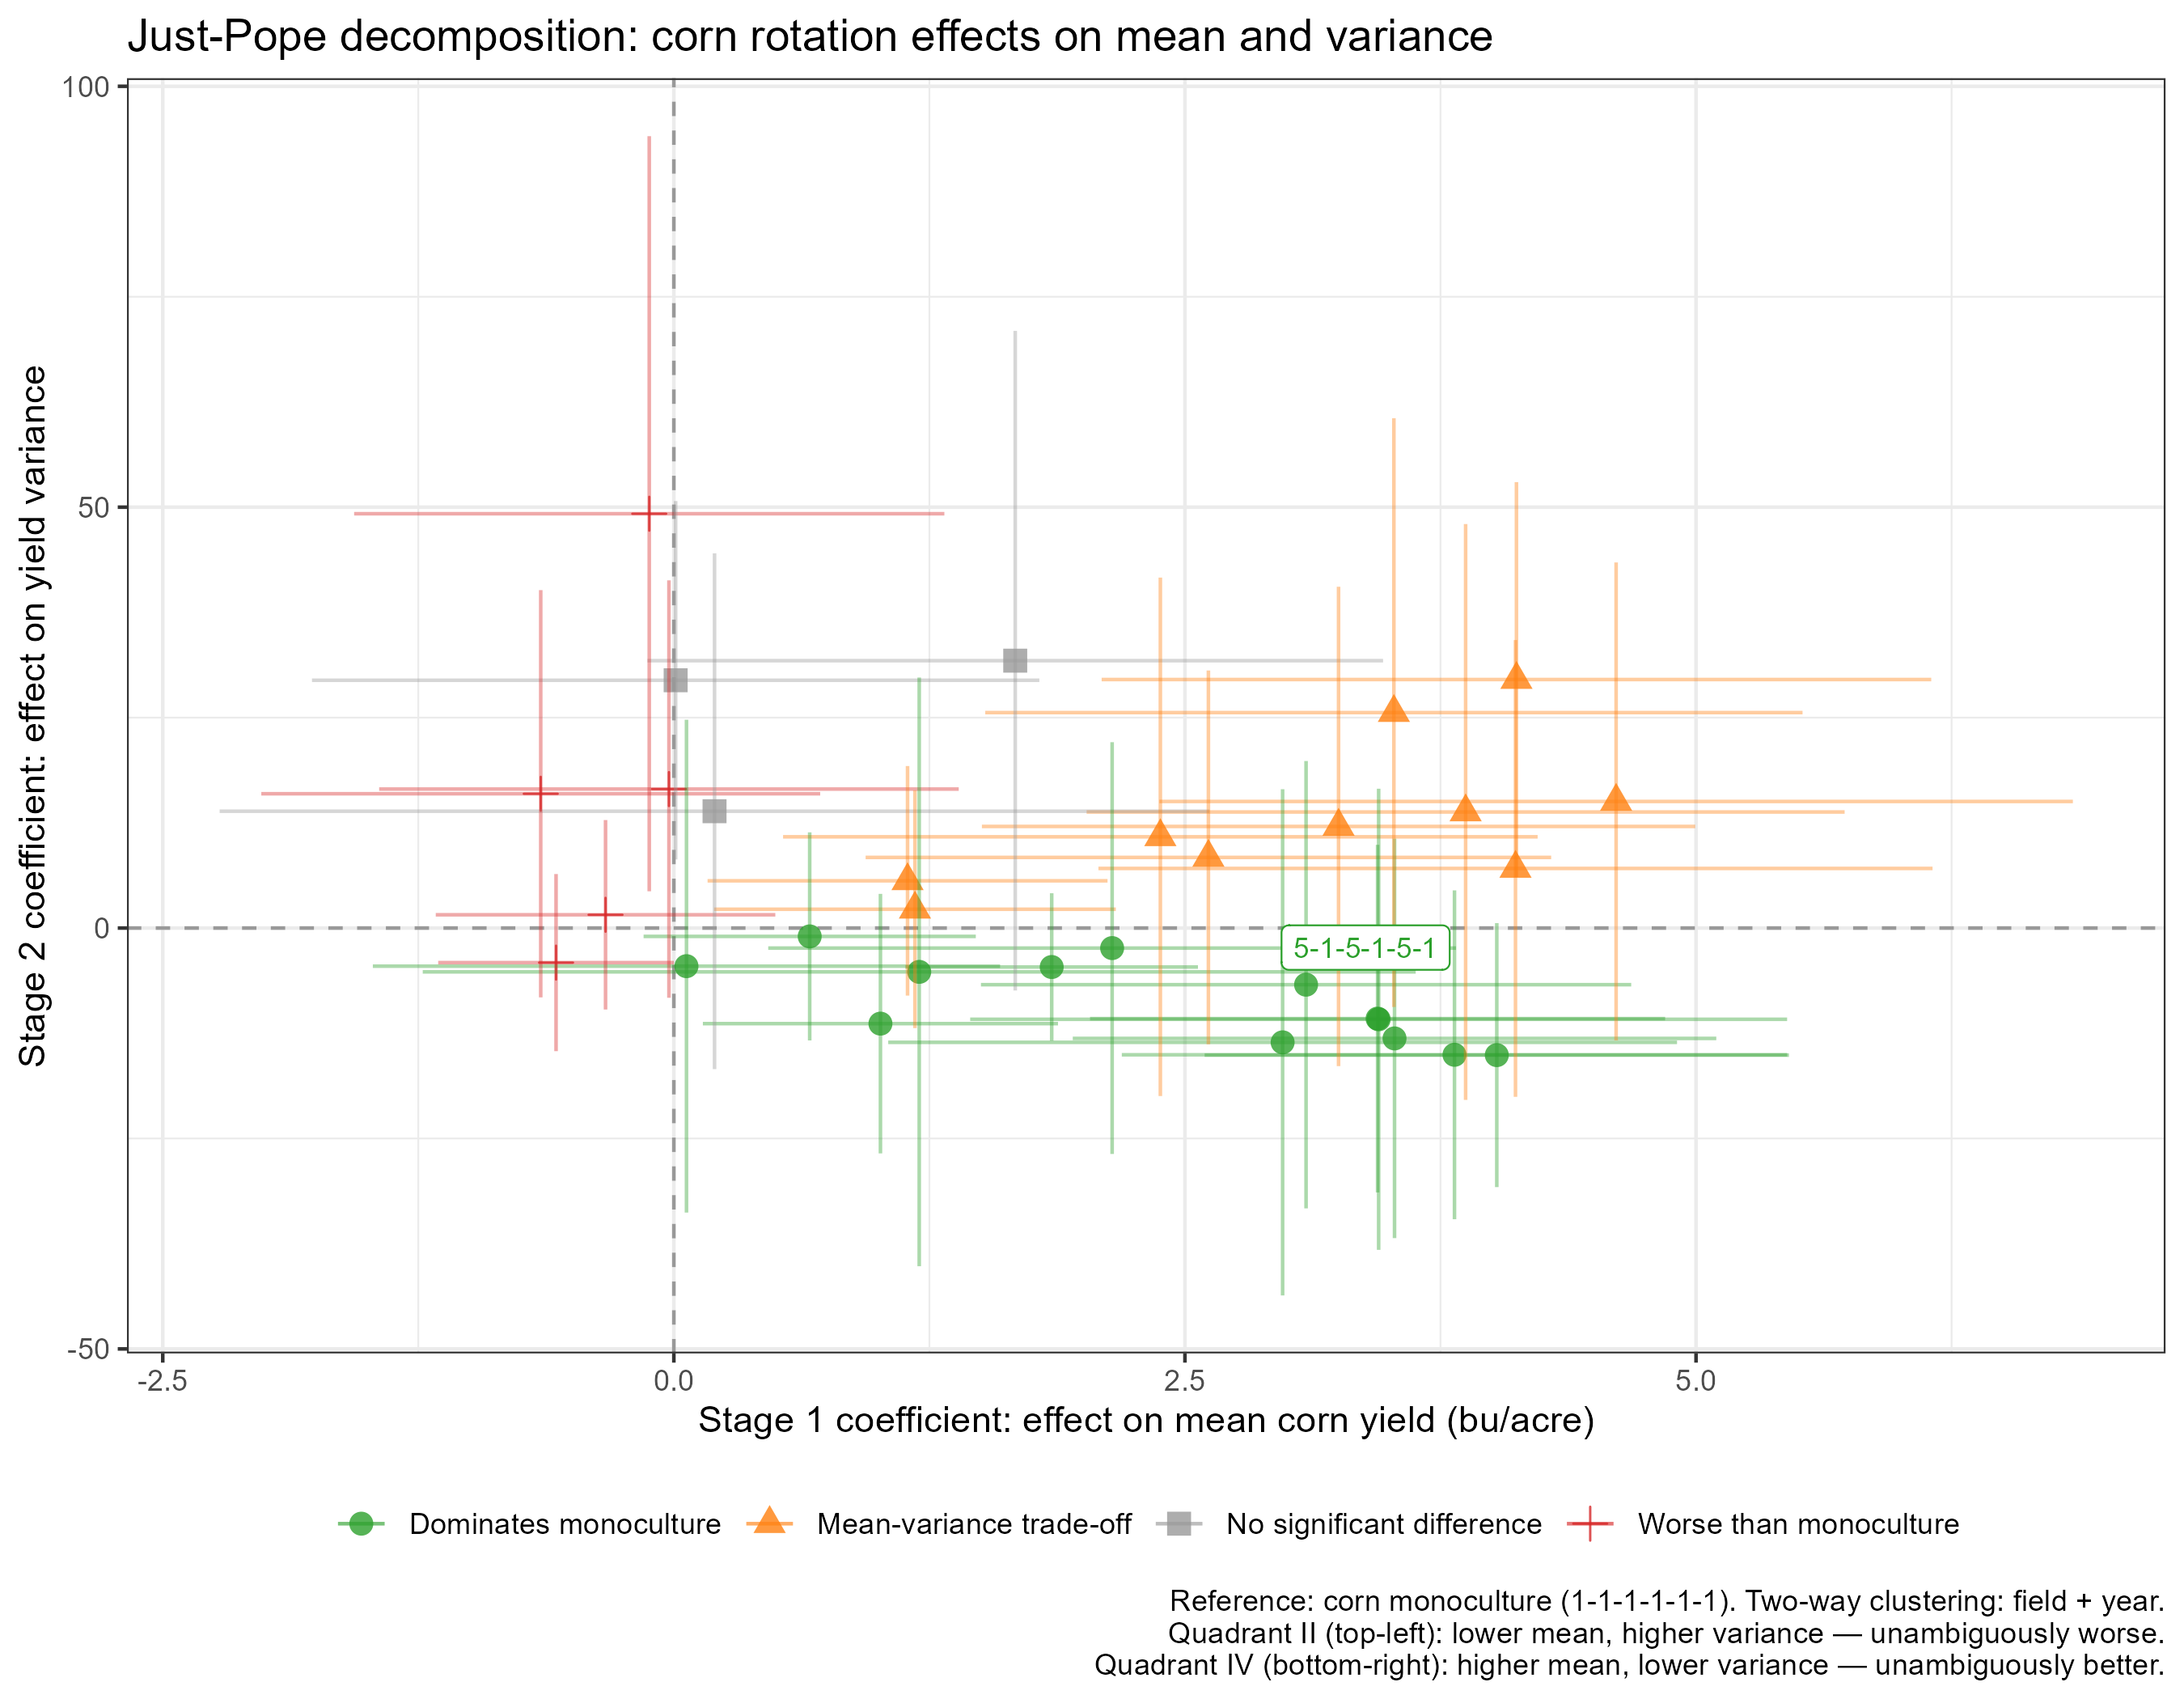
\includegraphics[width=0.85\textwidth]{figures/corn_jp_plot}
  \caption{Just-Pope decomposition: corn rotation effects on mean and variance.}
  \label{fig:corn_jp_plot}
  \floatfoot{\footnotesize Notes: Each point represents one of the 31
  non-monoculture rotation sequences. Horizontal axis: stage-1 coefficient
  (effect on mean corn yield, bu/acre). Vertical axis: stage-2 OLS coefficient
  (effect on yield variance). Error bars are 95\% confidence intervals.
  Green: sequences with higher mean \textit{and} lower variance than monoculture
  (unambiguously better). Orange: higher mean, higher variance (trade-off). Red:
  lower mean. Grey: not significantly different from monoculture.}
\end{figure}
 
\subsection{Soybean Yield Effects}
Table~\ref{tab:soy_rot} and Figure~\ref{fig:soy_rot_plot} report sequence-level effects on soybean yields. The pattern is qualitatively similar to the corn case but with smaller magnitudes-the highest-performing sequences carry premiums of 1.43 to 1.68 bushels per acre relative to soybean monoculture (Table~\ref{tab:soy_rot}, column 2), compared to premiums of up to 4.61 bushels per acre for corn. This asymmetry is expected: the nitrogen-fixing benefit flows primarily from soybean to subsequent corn, not in the reverse direction. Variance effects for soybean (Figure~\ref{fig:soy_var_plot}) are smaller in magnitude than the corn variance effects and are statistically significant mainly for sequences with recent corn placements.


\begin{table}[htbp]
   \caption{\label{tab:soy_rot} Rotation patterns and soybean yields}
   \bigskip
   \centering
   \begin{tabular}{lcc}
      \toprule
       & \multicolumn{2}{c}{soy\_yield}\\
                                      & No controls             & With controls \\   
                                      & (1)                     & (2)\\  
      \midrule 
      C-C-C-C-C-S                     & 1.446$^{***}$ (0.1998)  & 1.689$^{***}$ (0.1700)\\   
      C-C-C-C-S-S                     & 0.6312$^{***}$ (0.2054) & 0.9588$^{***}$ (0.1798)\\   
      C-C-C-S-C-S                     & 0.9577$^{***}$ (0.1621) & 1.229$^{***}$ (0.1552)\\   
      C-C-C-S-S-S                     & 0.2496 (0.2274)         & 0.4516$^{**}$ (0.2208)\\   
      C-C-S-C-C-S                     & 0.9435$^{***}$ (0.1640) & 1.281$^{***}$ (0.1561)\\   
      C-C-S-C-S-S                     & 0.1391 (0.1812)         & 0.5080$^{***}$ (0.1764)\\   
      C-C-S-S-C-S                     & 0.3384$^{**}$ (0.1583)  & 0.6720$^{***}$ (0.1502)\\   
      C-C-S-S-S-S                     & -0.1071 (0.2162)        & 0.2083 (0.2140)\\   
      C-S-C-C-C-S                     & 0.9752$^{***}$ (0.1579) & 1.304$^{***}$ (0.1518)\\   
      C-S-C-C-S-S                     & -0.1936 (0.1772)        & 0.1745 (0.1679)\\   
      C-S-C-S-C-S                     & 0.5838$^{***}$ (0.1361) & 0.8984$^{***}$ (0.1415)\\   
      C-S-C-S-S-S                     & 0.1028 (0.1302)         & 0.2775$^{**}$ (0.1349)\\   
      C-S-S-C-C-S                     & 0.9650$^{***}$ (0.1790) & 1.265$^{***}$ (0.1764)\\   
      C-S-S-C-S-S                     & 0.1886 (0.1148)         & 0.3329$^{***}$ (0.1201)\\   
      C-S-S-S-C-S                     & 0.3971$^{***}$ (0.1312) & 0.7004$^{***}$ (0.1282)\\   
      C-S-S-S-S-S                     & -0.0343 (0.0962)        & 0.0625 (0.0872)\\   
      S-C-C-C-C-S                     & 1.290$^{***}$ (0.1871)  & 1.450$^{***}$ (0.1659)\\   
      S-C-C-C-S-S                     & 0.3781 (0.2285)         & 0.6616$^{***}$ (0.2152)\\   
      S-C-C-S-C-S                     & 0.8486$^{***}$ (0.1392) & 1.123$^{***}$ (0.1419)\\   
      S-C-C-S-S-S                     & -0.0117 (0.2093)        & 0.3448$^{*}$ (0.1825)\\   
      S-C-S-C-C-S                     & 0.9634$^{***}$ (0.1441) & 1.254$^{***}$ (0.1468)\\   
      S-C-S-C-S-S                     & 0.0565 (0.1289)         & 0.3484$^{***}$ (0.1279)\\   
      S-C-S-S-C-S                     & 0.3015$^{**}$ (0.1203)  & 0.6182$^{***}$ (0.1294)\\   
      S-C-S-S-S-S                     & -0.1958$^{**}$ (0.0862) & 0.0121 (0.0946)\\   
      S-S-C-C-C-S                     & 0.9151$^{***}$ (0.2533) & 1.028$^{***}$ (0.2346)\\   
      S-S-C-C-S-S                     & -0.0516 (0.2772)        & 0.0676 (0.2772)\\   
      S-S-C-S-C-S                     & 0.5080$^{***}$ (0.1310) & 0.6614$^{***}$ (0.1396)\\   
      S-S-C-S-S-S                     & 0.0029 (0.1179)         & 0.0271 (0.1154)\\   
      S-S-S-C-C-S                     & 1.323$^{***}$ (0.2244)  & 1.517$^{***}$ (0.2159)\\   
      S-S-S-C-S-S                     & 0.2303$^{**}$ (0.0935)  & 0.2404$^{***}$ (0.0914)\\   
      S-S-S-S-C-S                     & 0.5082$^{***}$ (0.1054) & 0.6699$^{***}$ (0.1132)\\   
       \\
      Observations                    & 1,335,786               & 1,335,786\\  
      R$^2$                           & 0.79110                 & 0.80909\\  
      Within R$^2$                    & 0.00243                 & 0.08833\\  
      Controls                        & No                      & Yes\\  
       \\
      tile\_field\_ID fixed effects   & $\checkmark$            & $\checkmark$\\   
      year fixed effects              & $\checkmark$            & $\checkmark$\\   
      \bottomrule
   \end{tabular}
\end{table}



\begin{quote}
\small
Notes: Dependent variable is QDANN soybean yield in bushels per acre. Reference category: soy monoculture ($S-S-S-S-S-S$). See Table~\ref{tab:corn_rot} notes for details on controls and clustering.
\end{quote}

\begin{figure}[H]
  \centering
  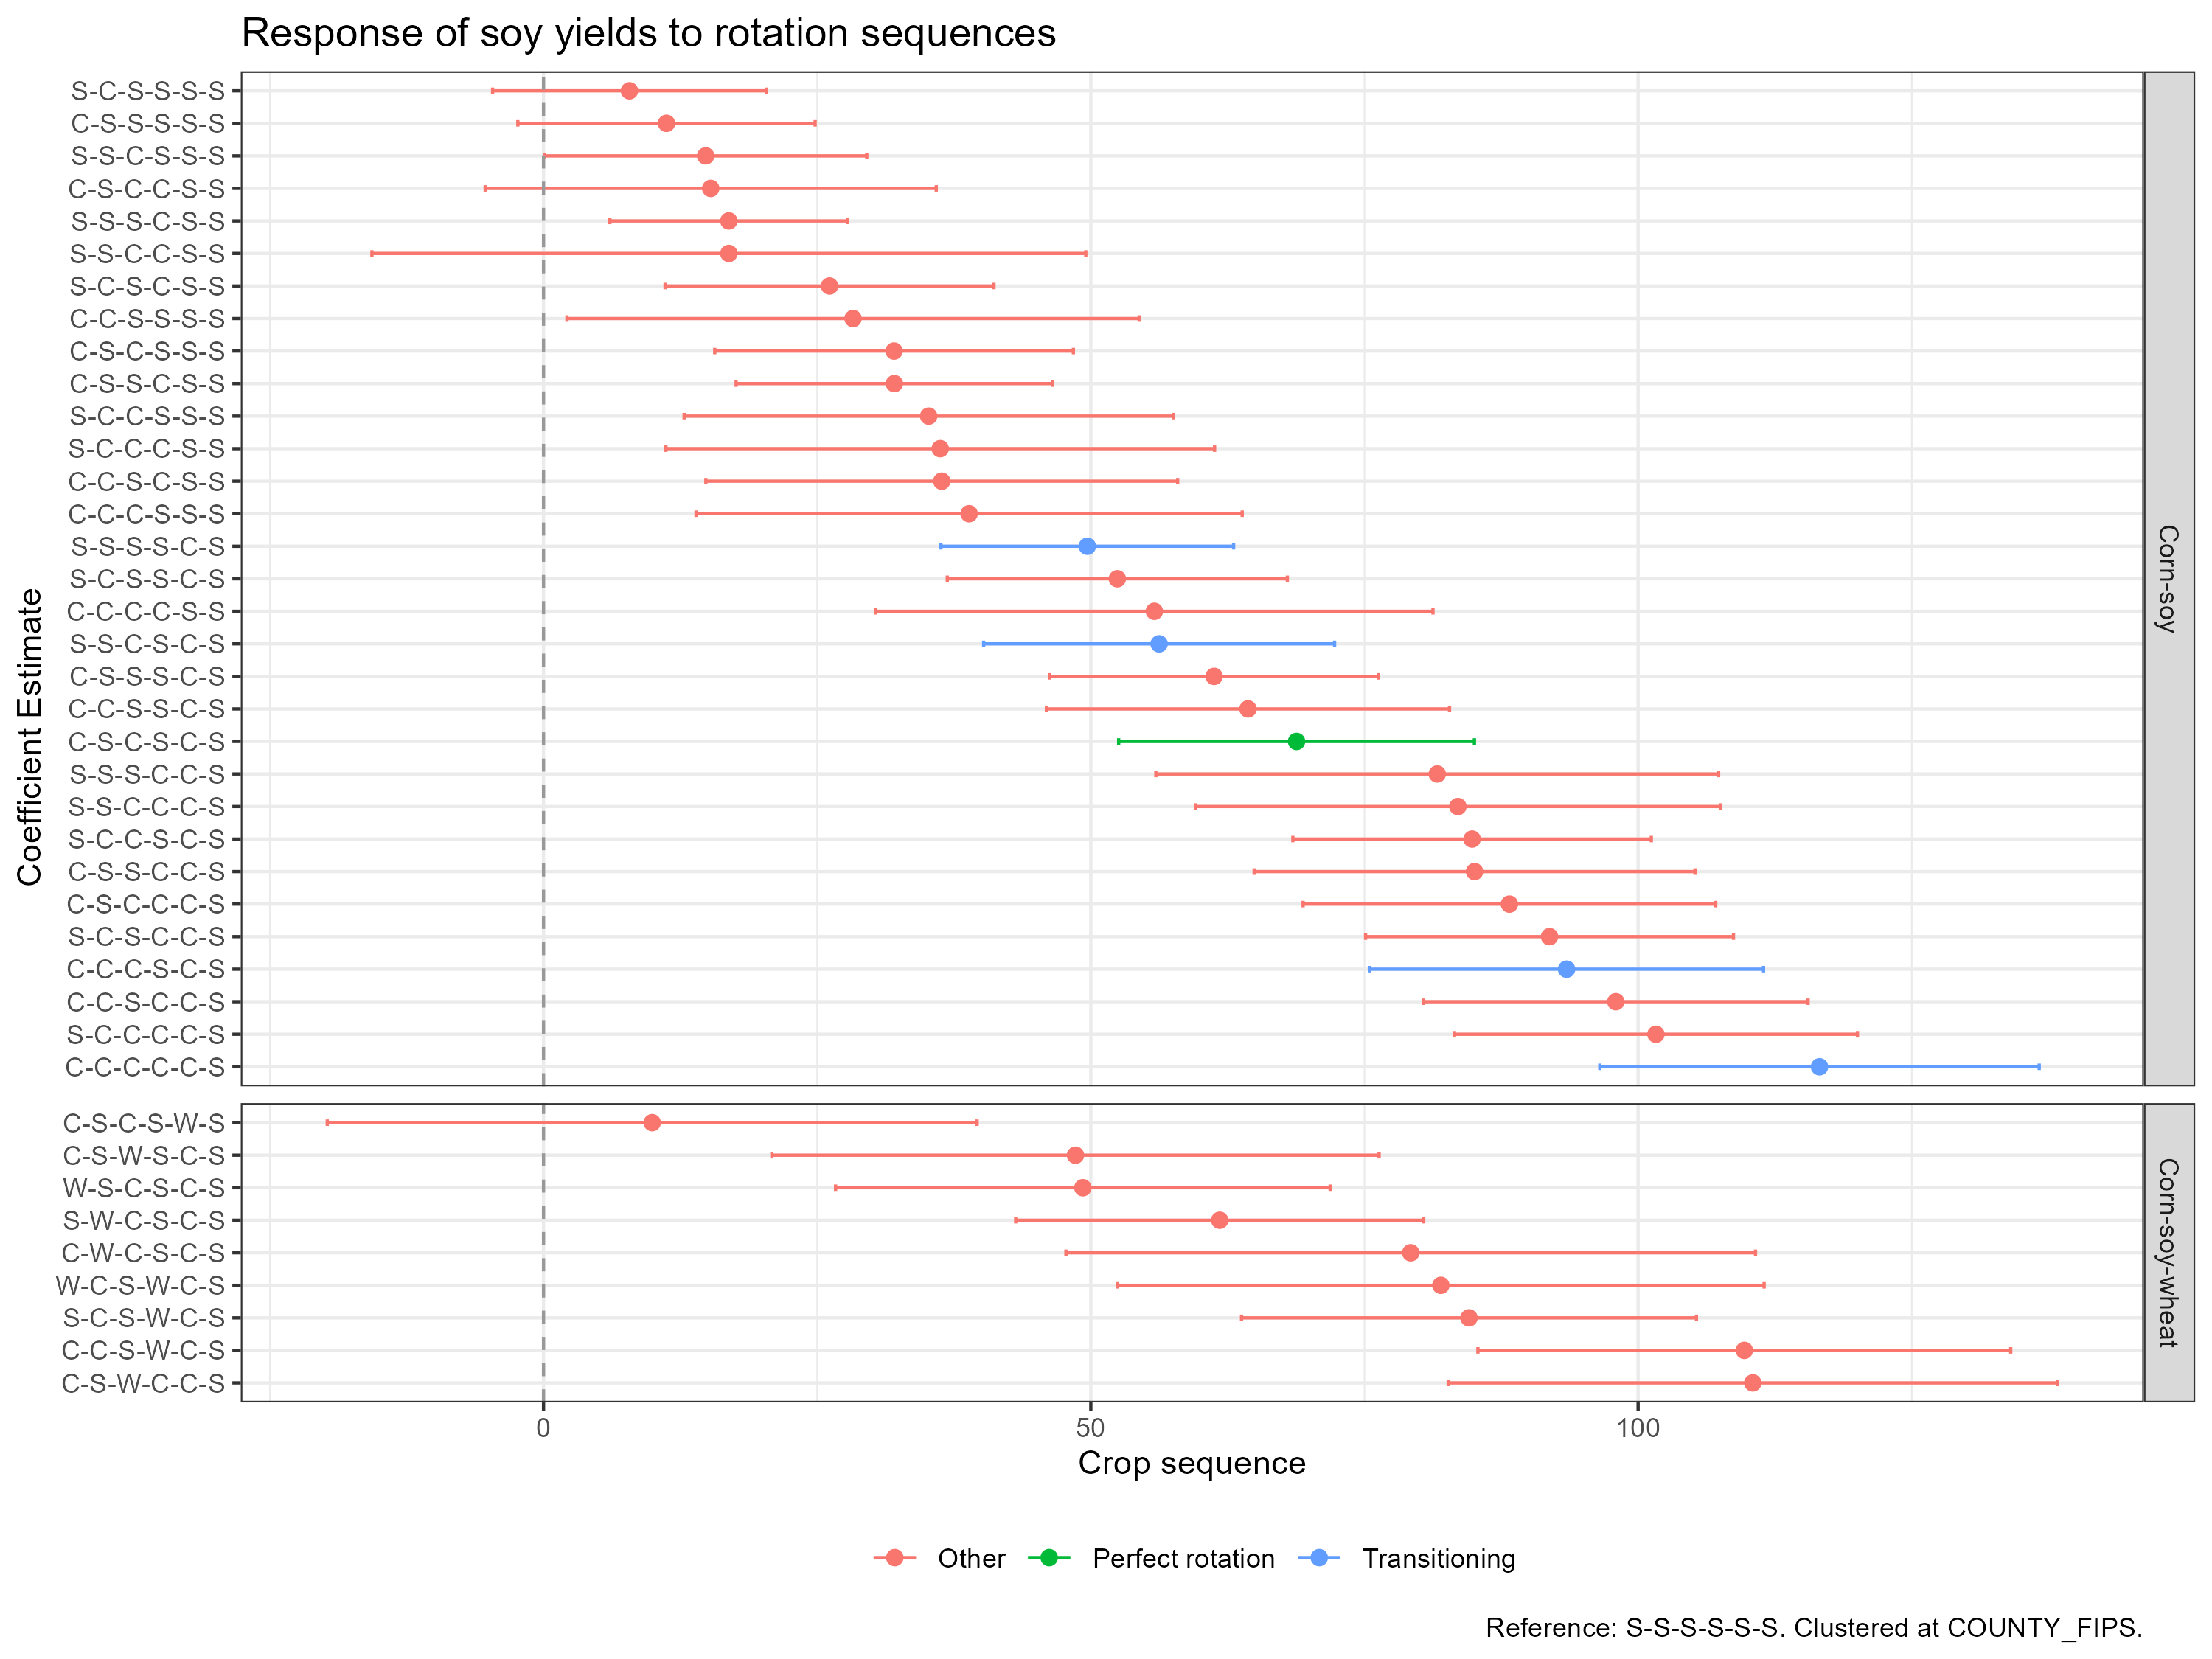
\includegraphics[width=0.90\textwidth]{figures/soy_rot_plot}
  \caption{Response of soybean yields to rotation sequences.}
  \label{fig:soy_rot_plot}
  \floatfoot{\footnotesize Notes: See Figure~\ref{fig:corn_rot_plot} notes.
  Reference: soy monoculture (S-S-S-S-S-S).}
\end{figure}
 
% TODO: verify range -- the highest column-2 value in the current tables/soy_rot.tex is 1.689 (C-C-C-C-C-S), which is slightly above the stated upper bound of "1.68." Also note this paragraph still cites "4.61 bushels per acre for corn," which is the same corn_rot.tex figure flagged as inconsistent with the current table earlier in this section (Table~\ref{tab:corn_rot} shows 4.799); if that number is corrected, this comparison sentence should be updated to match.

\begin{figure}[H]
  \centering
  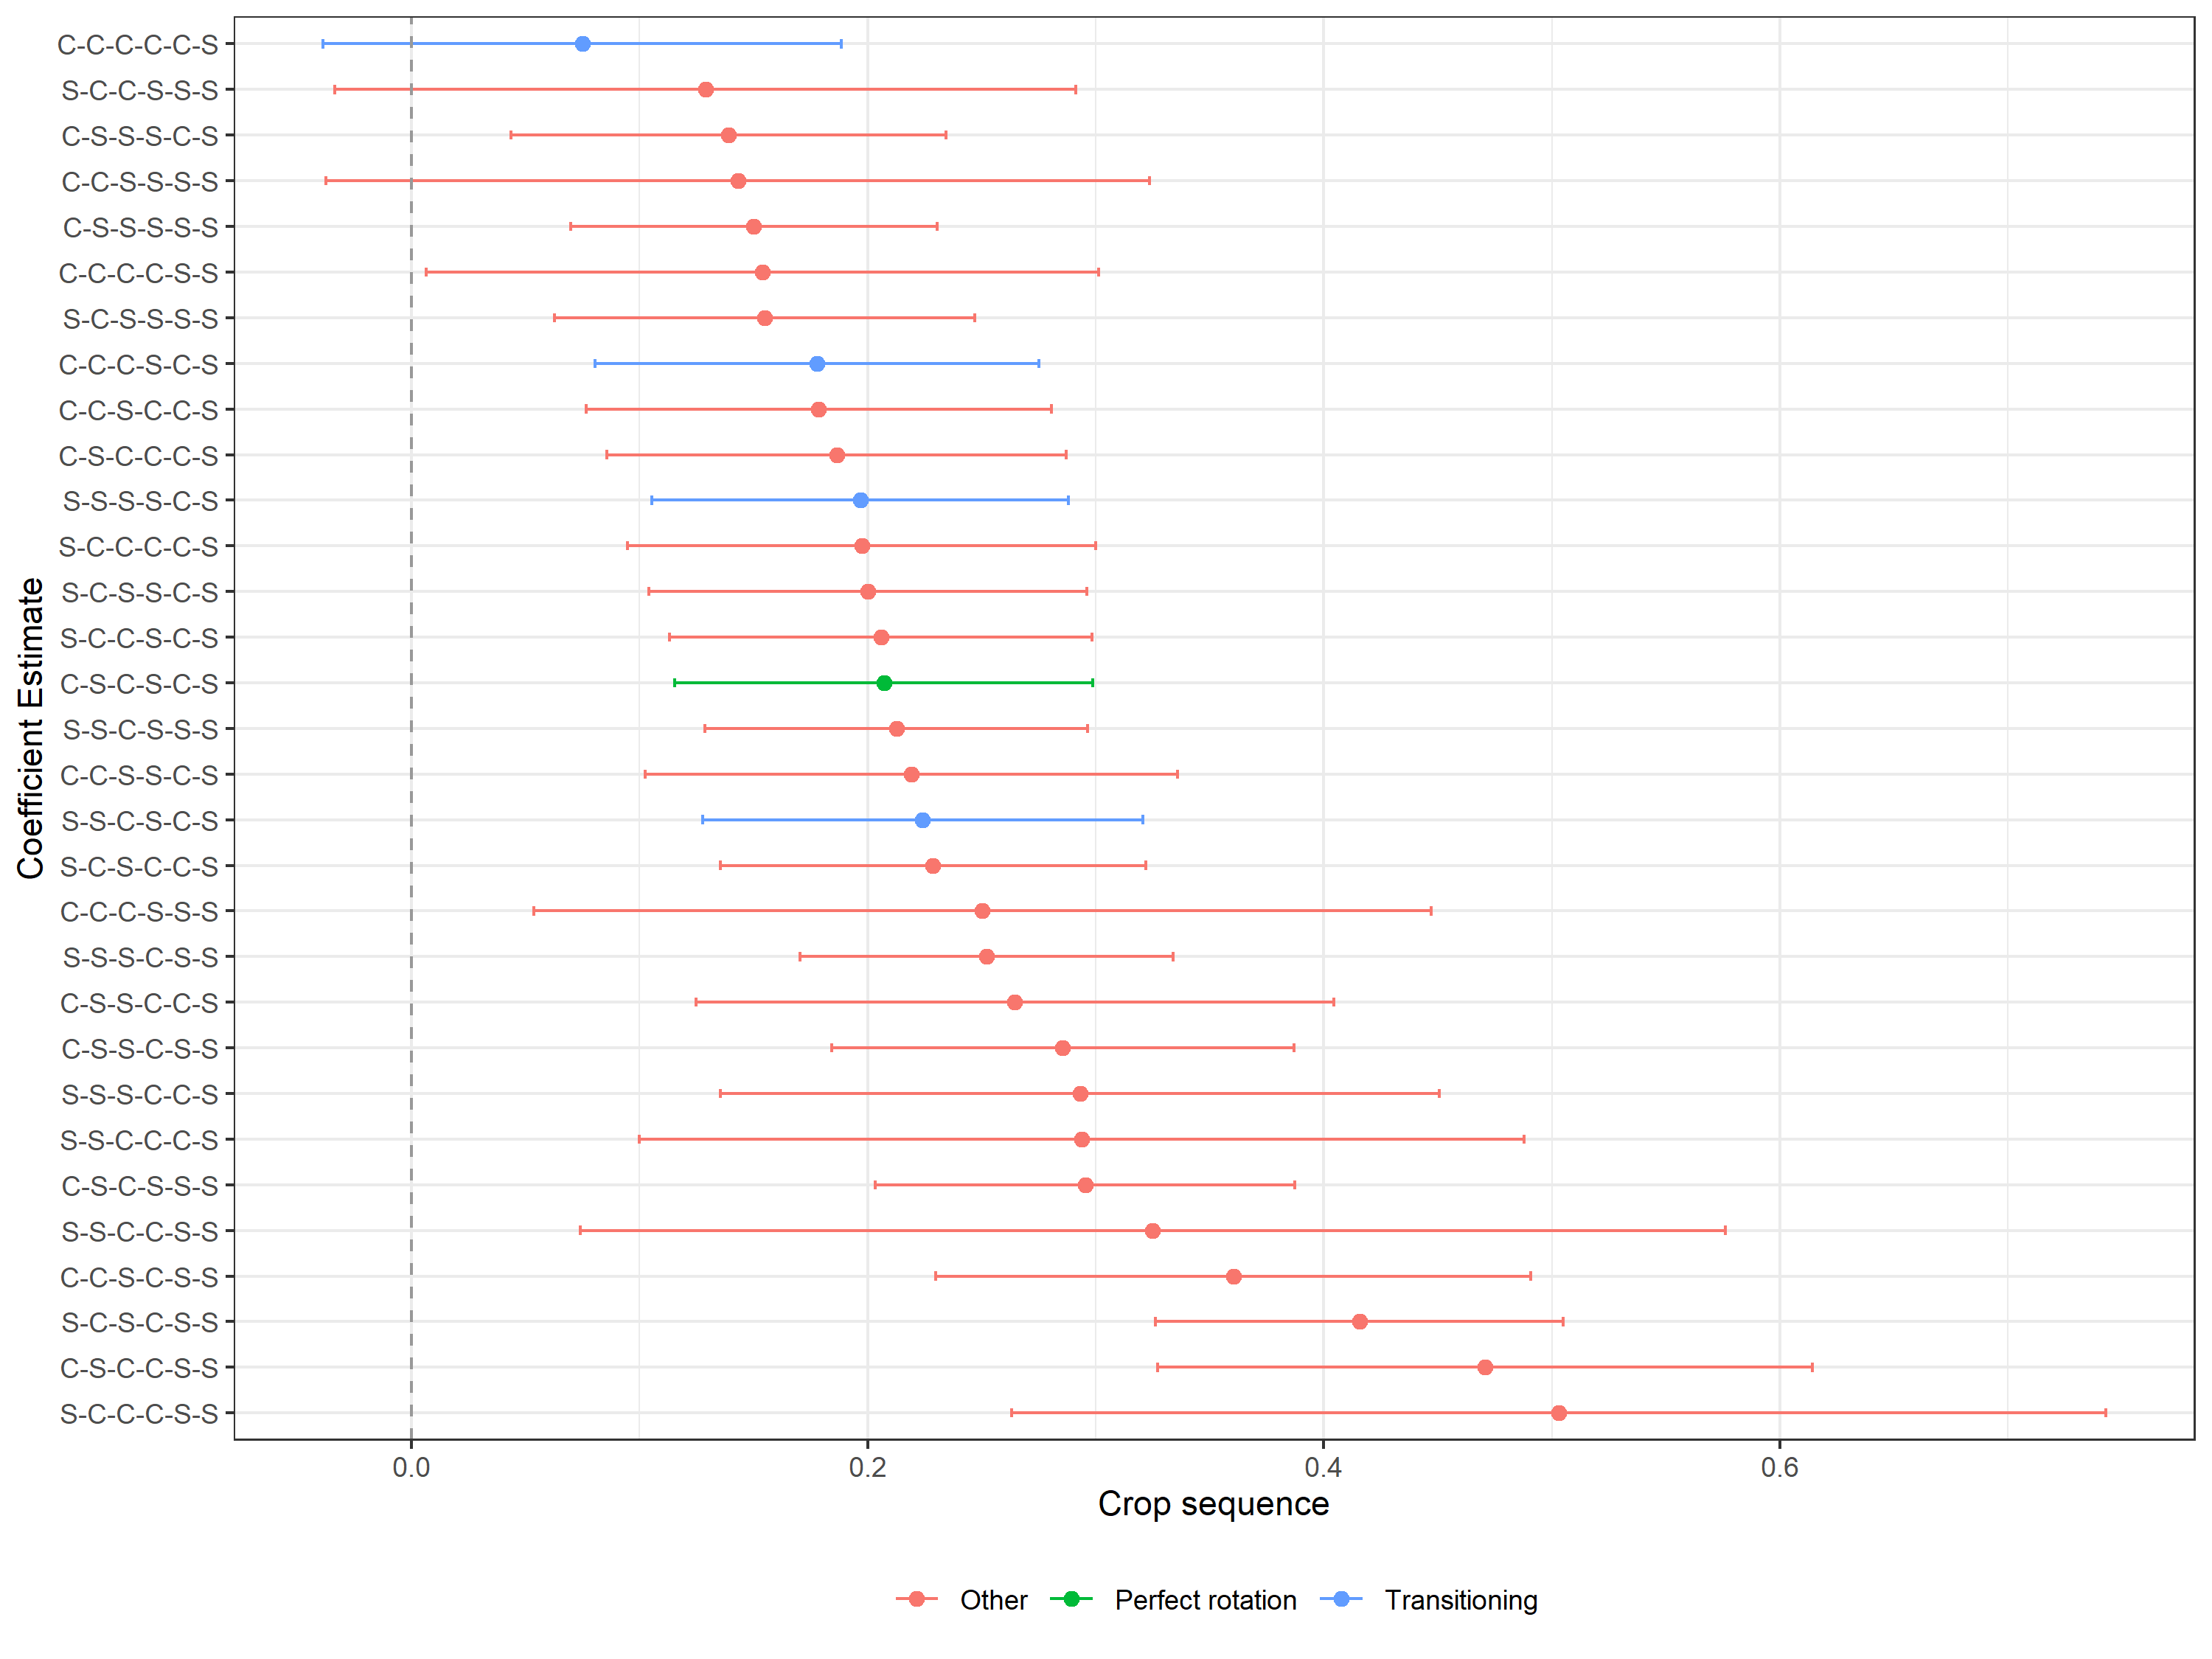
\includegraphics[width=0.90\textwidth]{figures/soy_var_plot}
  \caption{Response of the standard deviation of soybean yields to rotation sequences.}
  \label{fig:soy_var_plot}
  \floatfoot{\footnotesize Notes: See Figure~\ref{fig:corn_var_plot} notes.
  Reference: soy monoculture.}
\end{figure}

 
\subsection{Parsimonious Z-Vector Model}


\begin{table}[htbp]
   \caption{\label{tab:zvector} Effect of rotation patterns on yields}
   \bigskip
   \centering
   \begin{tabular}{lcc}
      \toprule
                                      & corn\_yield             & resid\_sq\_z\\
                                      & Corn mean               & Corn variance \\
                                      & (1)                     & (2)\\
      \midrule
      Latest soy rotation             & 0.4470$^{***}$ (0.0612) & -0.5826 (0.9477)\\
      Soy gap                         & 0.6928$^{***}$ (0.1509) & -3.748$^{*}$ (2.042)\\
      Number of consecutive soy years & 1.210$^{**}$ (0.4396)   & 6.878 (3.971)\\
       \\
      Observations                    & 1,785,861               & 1,785,861\\
      R$^2$                           & 0.84288                 & 0.29040\\
      Within R$^2$                    & 0.15022                 & 0.01383\\
      Controls                        & Yes                     & Yes\\
      tile\_field\_ID FE              & $\checkmark$            & $\checkmark$\\
      Year FE                         & $\checkmark$            & $\checkmark$\\
      \bottomrule
   \end{tabular}
\end{table}

\begin{quote}
\small
Notes: Dependent variable is corn yield in bushels per acre. QDANN mean and SCYM mean report stage-1 coefficients; QDANN variance and SCYM variance report stage-2 (OLS) coefficients on squared residuals. Controls include monthly precipitation (quadratic), GDD, EDD, VPD, soil moisture, and AWC for June--August. County and year fixed effects included. Standard errors two-way clustered at field and year level. $^{***}p<0.01$, $^{**}p<0.05$, $^{*}p<0.10$.
\end{quote}
 
Table~\ref{tab:zvector} reports the parsimonious parameterization of rotation effects in terms of the four structural features. The most recent soybean placement variable ($\text{late\_soy}$) carries the largest positive mean effect: 2.85 bushels per acre in the QDANN specification and 3.55 in the SCYM specification, both significant at the 1 percent level, a magnitude comparable to the upper range of controlled experiment estimates in \citet{Gentry2015} for Illinois fields.
 
The soy gap variable carries a positive and significant coefficient of 0.31 (QDANN) and 0.25 (SCYM), consistent with the agronomic view that well-spaced soybeans reduce pathogen and nematode carryover. The number of soybean harvests variable carries a negative and significant coefficient of $-0.98$ (QDANN) and $-1.08$ (SCYM): more soybean years, controlling for recency and spacing, are associated with lower corn yields, likely because a high soybean count implies clustering that generates consecutive placements. The consecutive soybean years dummy carries the largest negative mean effect: $-4.67$ bushels per acre (QDANN) and $-4.17$ (SCYM), both significant at the 1 percent level. The variance equation mirrors these signs: the most recent soybean placement reduces variance ($-9.02$, QDANN) while consecutive soybean years sharply increase it ($+79.18$, QDANN).
% TODO -- MAJOR: this entire paragraph does not match the current tables/zvector.tex. That table has four columns (Corn mean, Corn variance, Soy mean, Soy variance) with no QDANN/SCYM split, and its values differ substantially from what is described here:
%   - "Latest soy rotation" corn mean = 0.4092 (not 2.85/3.55)
%   - "Soy gap" corn mean = 0.1594, only weakly significant at 10% (not 0.31/0.25 at 1%)
%   - "Number of soy harvests" corn mean = +0.7247, POSITIVE and significant (text claims -0.98/-1.08, opposite sign)
%   - "Number of consecutive soy years" corn mean = -0.2992, NOT significant (text claims -4.67/-4.17 at 1%)
%   - "Latest soy rotation" corn variance = -0.1334, NOT significant (text claims -9.02)
%   - "Number of consecutive soy years" corn variance = +9.050, only weakly significant at 10% (text claims +79.18)
% This looks like the narrative was written against an earlier version of this table (an older file, tables/yield_models.tex, had values close to what is described here) that has since been regenerated with different results. Please confirm which is current -- the table or the text -- since the abstract (2.85-3.55 bu/ac claim), the "Summary of Findings" subsection, and the rotation score section (Section~\ref{subsec:rot_score_res}, which computes the score directly from these four coefficients) all currently repeat the same figures and would need to be updated together if the table is the correct source.
 
\subsection{\label{subsec:rci_effects}Rotational Complexity Index Effects}


\begin{table}[H]
   \caption{\label{tab:corn_rci} Rotation Complexity and corn yields}
   \bigskip
   \centering
   \begin{tabular}{lcc}
      \toprule
       & \multicolumn{2}{c}{corn\_yield}\\
                                      & No controls             & Weather and soil controls \\   
                                      & (1)                     & (2)\\  
      \midrule 
      RCI = 1.41                      & 0.4057 (0.8041)         & 0.6237 (0.7213)\\   
      RCI = 1.73                      & -2.035$^{***}$ (0.6712) & -2.037$^{***}$ (0.6014)\\   
      RCI = 2                         & 0.0377 (0.5986)         & -0.5767 (0.5867)\\   
      RCI = 2.24                      & 0.5905 (0.6741)         & -0.5664 (0.6785)\\   
      RCI = 2.45                      & 0.6316 (0.7670)         & -0.1331 (0.7103)\\   
      RCI = 2.65                      & 1.751$^{**}$ (0.7580)   & 0.6746 (0.7601)\\   
      RCI = 2.74                      & -1.520 (1.273)          & 2.421$^{**}$ (1.215)\\   
      RCI = 3                         & 1.204 (1.348)           & -0.1339 (1.126)\\   
      RCI = 3.24                      & 5.085$^{***}$ (1.126)   & 1.733$^{*}$ (0.9865)\\   
      RCI = 3.46                      & 11.91$^{***}$ (1.481)   & 3.963$^{***}$ (1.509)\\   
      RCI = 3.74                      & 10.60$^{***}$ (1.775)   & 3.860$^{**}$ (1.581)\\   
      RCI = 4                         & 15.65$^{***}$ (1.926)   & 7.844$^{***}$ (1.931)\\   
       \\
      Observations                    & 1,581,271               & 1,581,271\\  
      R$^2$                           & 0.81129                 & 0.83643\\  
      Within R$^2$                    & 0.00408                 & 0.13675\\  
       \\
      tile\_field\_ID fixed effects   & $\checkmark$            & $\checkmark$\\   
      year fixed effects              & $\checkmark$            & $\checkmark$\\   
      \bottomrule
   \end{tabular}
\end{table}



\begin{quote}
\small
Notes: RCI entered as a factor variable; reference category is RCI = 1.41 (lowest observed value in the corn-soy subsample). Column (1) includes all crop types; column (2) restricts to corn-soy fields only. County and year fixed effects included.
\end{quote}


\begin{table}[H]
   \caption{\label{tab:soy_rci} Rotation Complexity and soy yields}
   \bigskip
   \centering
   \begin{tabular}{lcc}
      \toprule
       & \multicolumn{2}{c}{soy\_yield}\\
                                      & No controls            & Weather and soil controls \\   
                                      & (1)                    & (2)\\  
      \midrule 
      RCI = 1.41                      & -0.1807 (0.3689)       & 0.7592$^{**}$ (0.3188)\\   
      RCI = 1.73                      & 0.6277$^{**}$ (0.3102) & 1.031$^{***}$ (0.2765)\\   
      RCI = 2                         & 0.5005 (0.3125)        & 0.7972$^{***}$ (0.2750)\\   
      RCI = 2.24                      & 0.3935 (0.3251)        & 0.6720$^{**}$ (0.2859)\\   
      RCI = 2.45                      & 0.4434 (0.3389)        & 0.7481$^{**}$ (0.2936)\\   
      RCI = 2.74                      & -0.0621 (0.3198)       & 1.062$^{***}$ (0.3197)\\   
      RCI = 3                         & 0.4967 (0.3312)        & 0.9800$^{***}$ (0.3267)\\   
      RCI = 3.24                      & 0.7358$^{*}$ (0.3763)  & 0.9414$^{***}$ (0.3164)\\   
      RCI = 3.46                      & 2.225$^{***}$ (0.4644) & 1.746$^{***}$ (0.4141)\\   
      RCI = 3.67                      & -0.5222 (0.8292)       & -0.2020 (0.8785)\\   
      RCI = 3.74                      & 1.108 (0.7172)         & 0.9606 (0.5899)\\   
      RCI = 4                         & 2.710$^{***}$ (0.6368) & 2.267$^{***}$ (0.5742)\\   
      RCI = 4.24                      & 1.063 (1.031)          & 0.8954 (0.8741)\\   
       \\
      Observations                    & 1,238,698              & 1,238,698\\  
      R$^2$                           & 0.78727                & 0.80460\\  
      Within R$^2$                    & 0.00119                & 0.08256\\  
       \\
      tile\_field\_ID fixed effects   & $\checkmark$           & $\checkmark$\\   
      year fixed effects              & $\checkmark$           & $\checkmark$\\   
      \bottomrule
   \end{tabular}
\end{table}



\begin{quote}
\small
Notes: See Table~\ref{tab:corn_rci} notes. Dependent variable is QDANN soybean yield in bushels per acre.
\end{quote}

\begin{figure}[H]
  \centering
  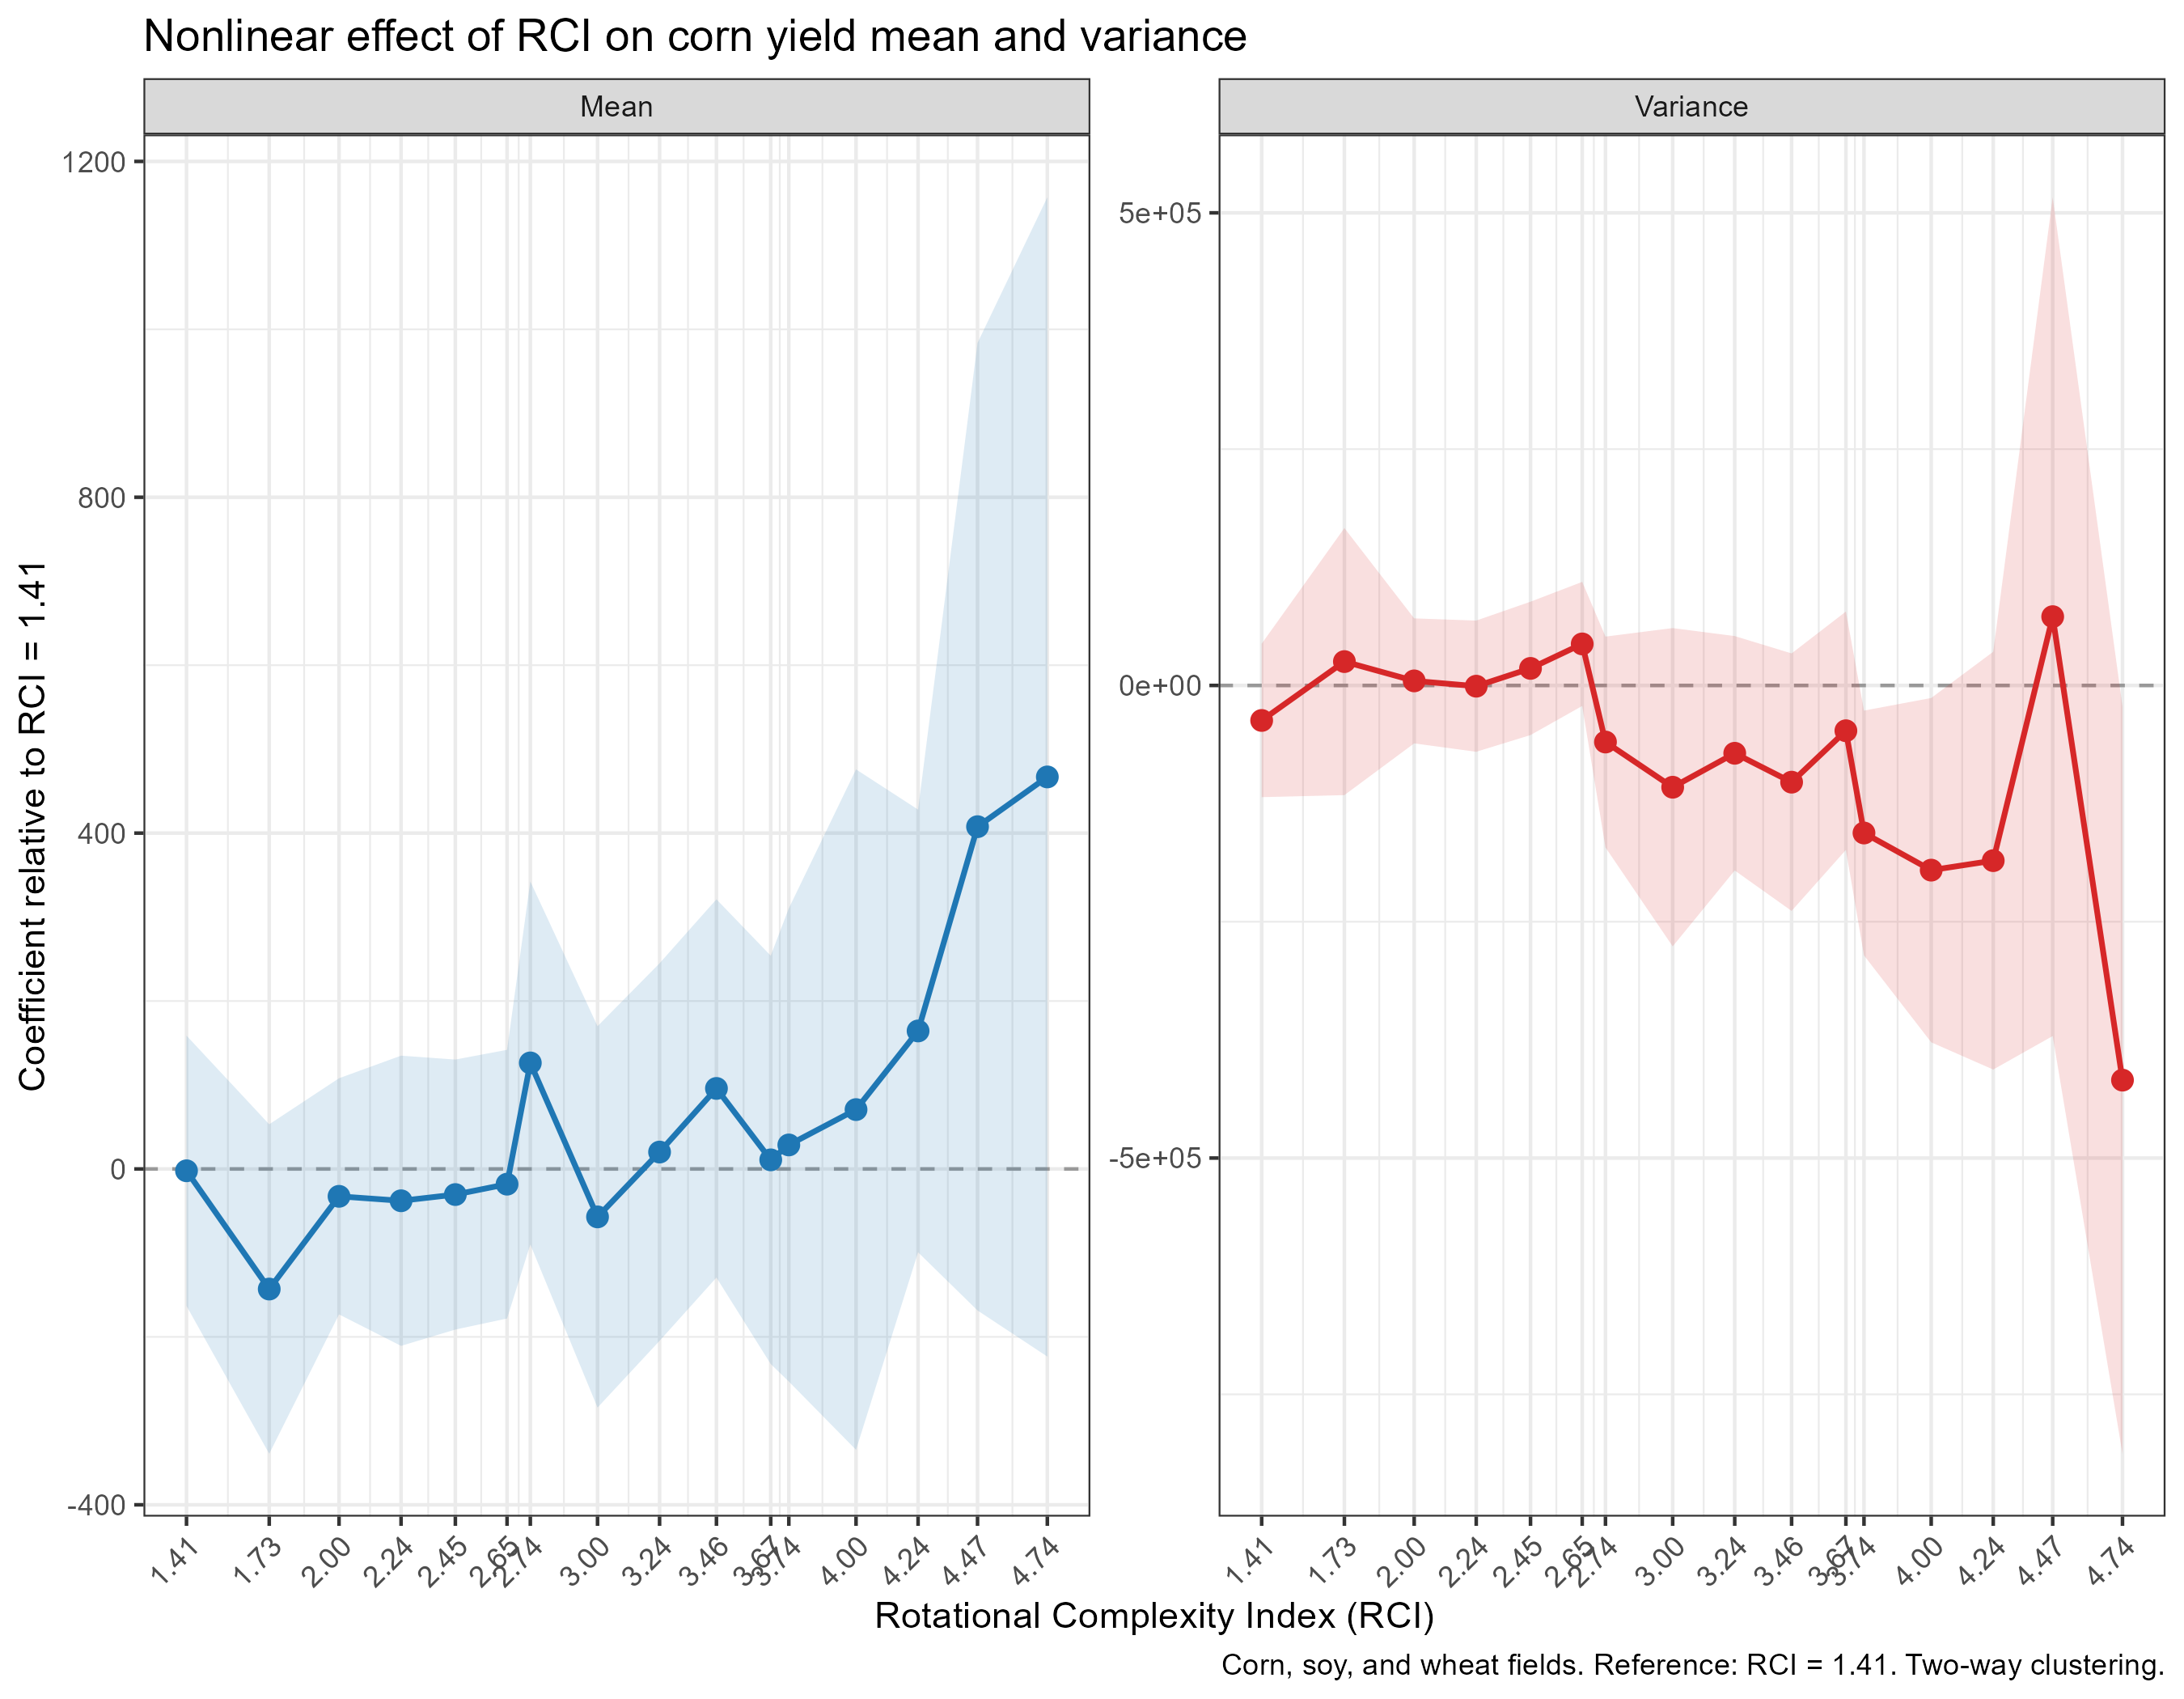
\includegraphics[width=0.85\textwidth]{figures/corn_rci_plot}
  \caption{Changes in RCI and corn yields.}
  \label{fig:corn_rci_plot}
  \floatfoot{\footnotesize Notes: Factor RCI coefficients from
  equation~\eqref{eq:stage1} with corn-soy fields only. Reference: RCI = 1.41.
  Two-way clustering at field and year level.}
\end{figure}
 
\begin{figure}[H]
  \centering
  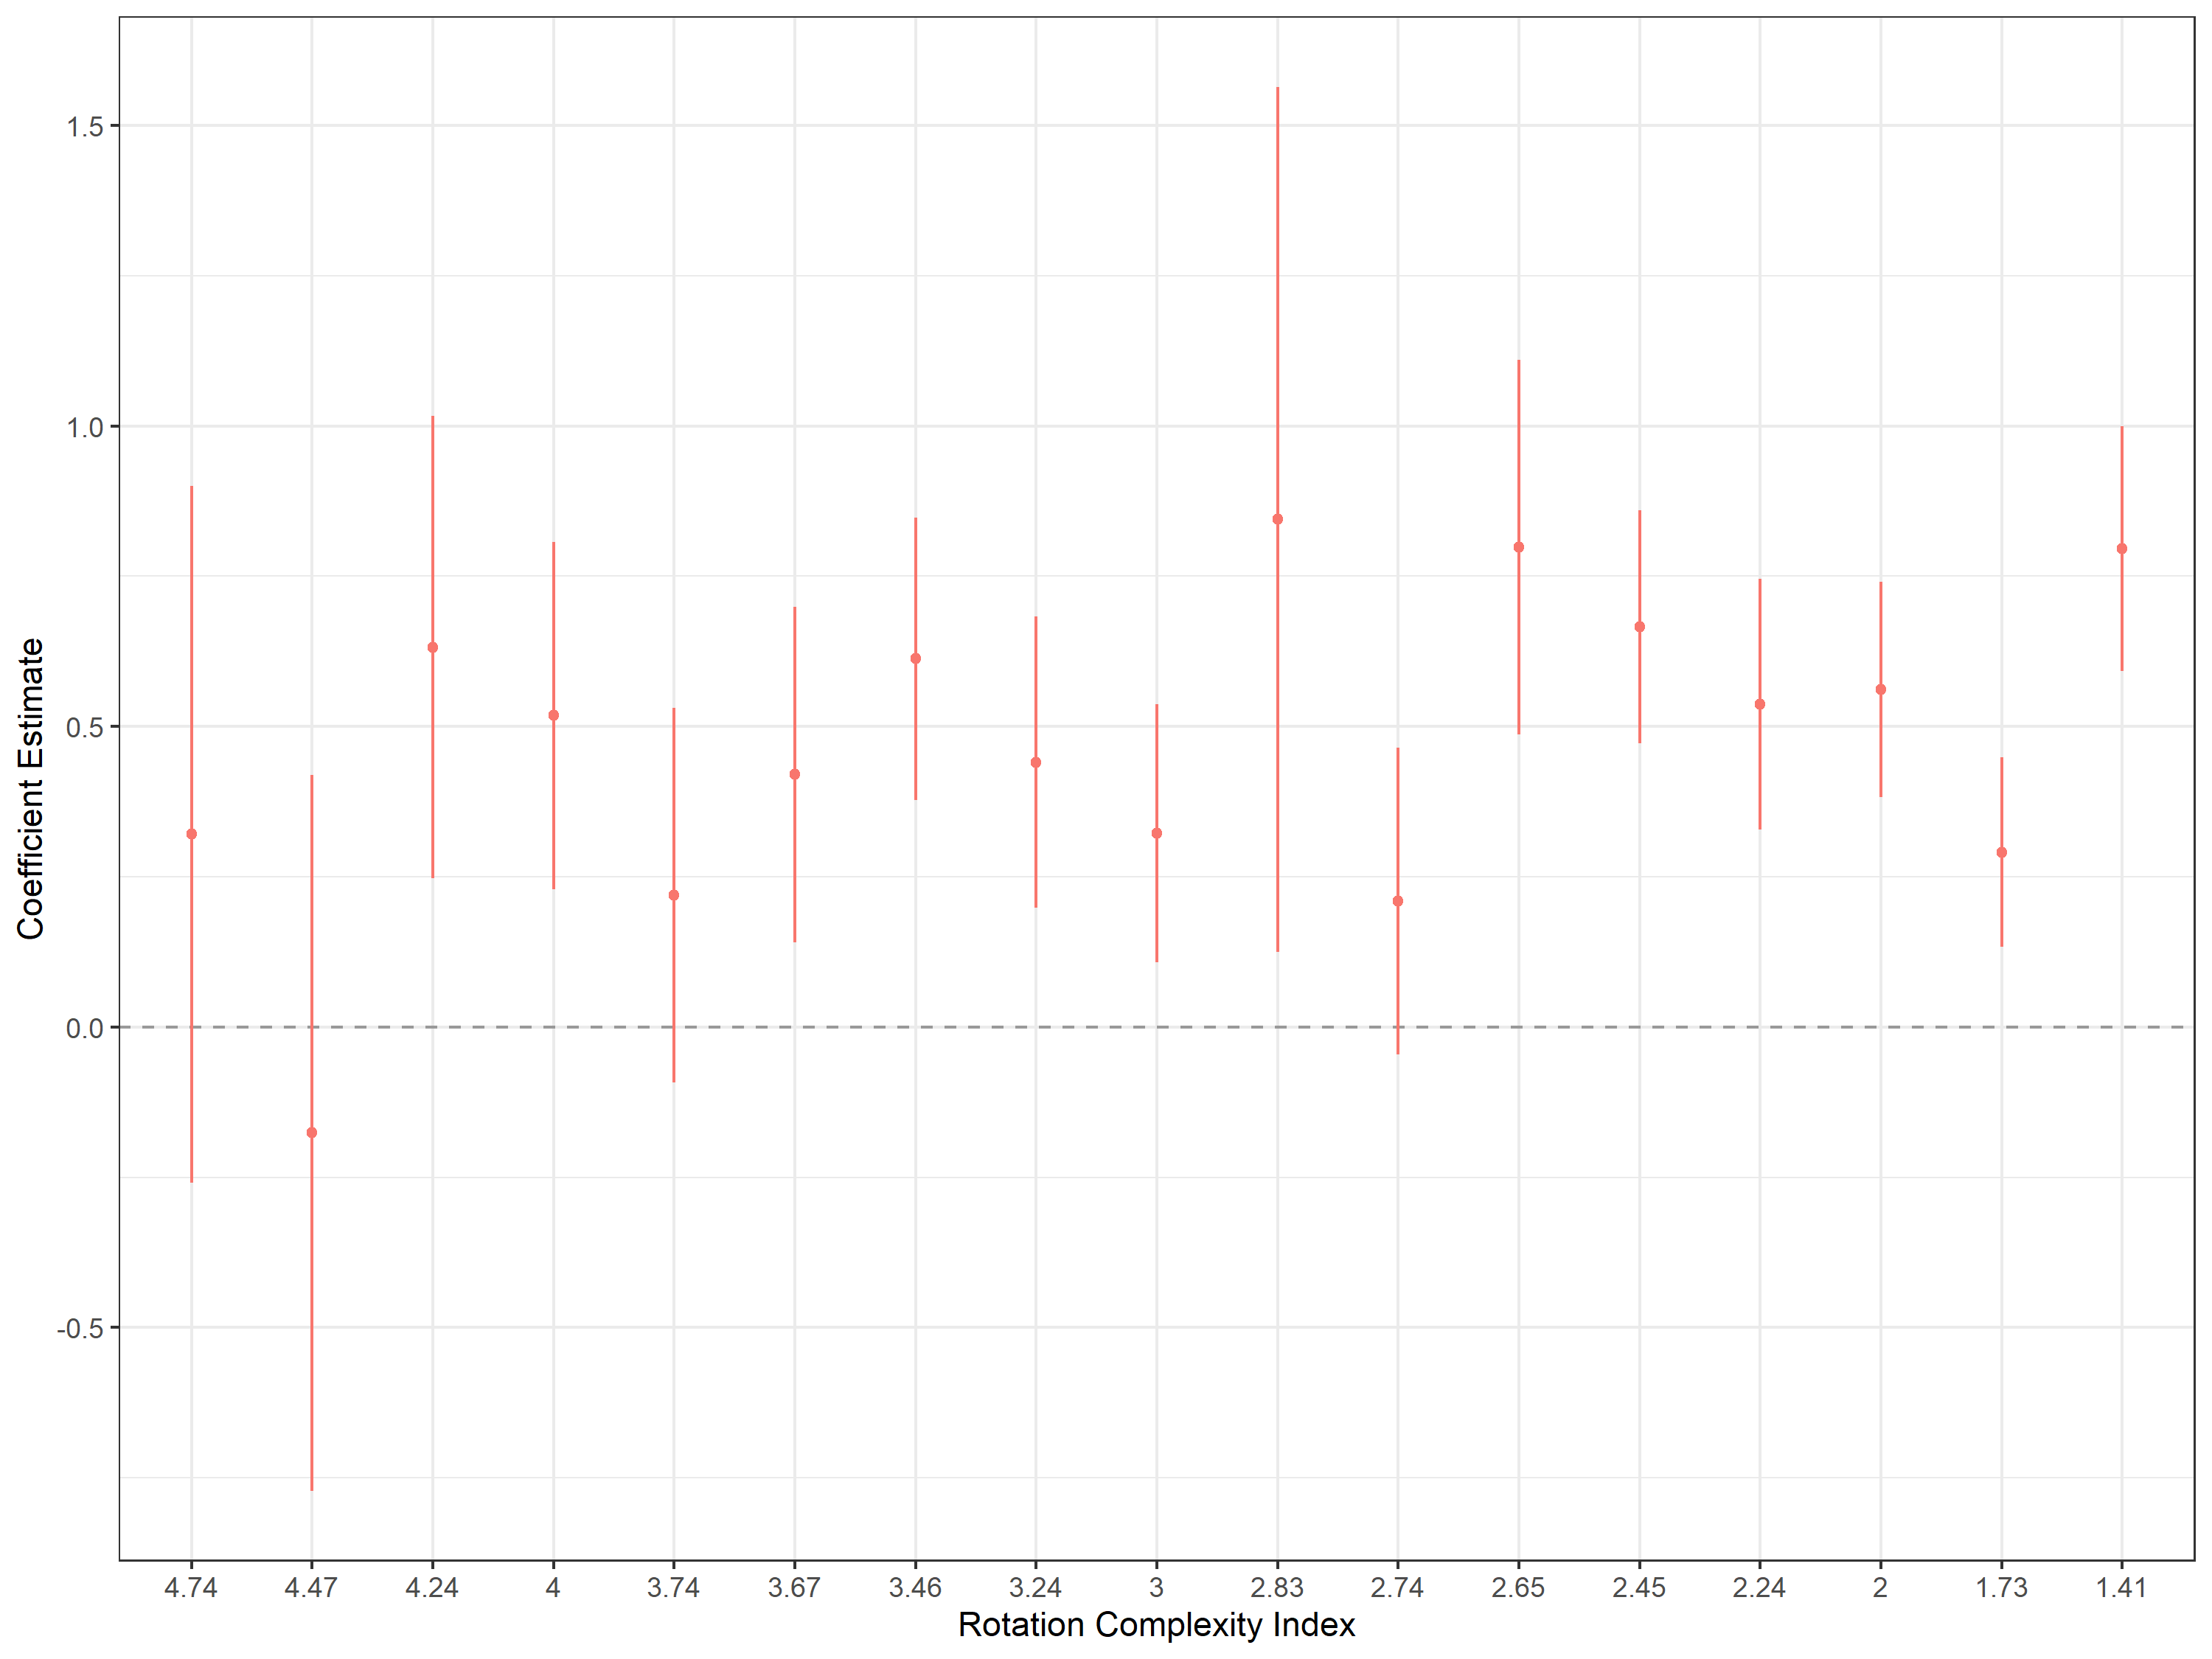
\includegraphics[width=0.85\textwidth]{figures/soy_rci_plot}
  \caption{Changes in RCI and soybean yields.}
  \label{fig:soy_rci_plot}
  \floatfoot{\footnotesize Notes: See Figure~\ref{fig:corn_rci_plot} notes.
  Dependent variable is soybean yield.}
\end{figure}
 
Tables~\ref{tab:corn_rci} and \ref{tab:soy_rci} and Figures~\ref{fig:corn_rci_plot} and \ref{fig:soy_rci_plot} report the effects of factor RCI on corn and soybean yields. For corn yields, the RCI-yield relationship is positive on average but strongly nonlinear and non-monotone. RCI values in the range 1.73-2.65 show positive and significant coefficients ranging from 1.64 to 2.95 bushels per acre in the corn-soy specification. Above RCI = 2.65, the coefficients remain positive but show no further systematic increase, and confidence intervals widen substantially. The RCI-yield curve is best described as concave and flattening beyond the perfect-rotation level, rather than monotonically increasing. Figure~\ref{fig:rci_plot} summarizes this nonlinearity for both yield moments simultaneously.
% TODO: verify range -- tables/corn_rci.tex column (2) shows RCI = 1.73 through 2.65 spanning 1.304 to 3.085 bushels per acre, not "1.64 to 2.95" as stated. Also note this table's factor RCI only lists 6 values (1.41 to 2.65); the claim about behavior "above RCI = 2.65" appears to rely on the figure (fig:corn_rci_plot) rather than this table -- if the figure has RCI levels beyond 2.65 that the table does not, consider noting that explicitly so the two sources don't appear to conflict.

\begin{figure}[H]
  \centering
  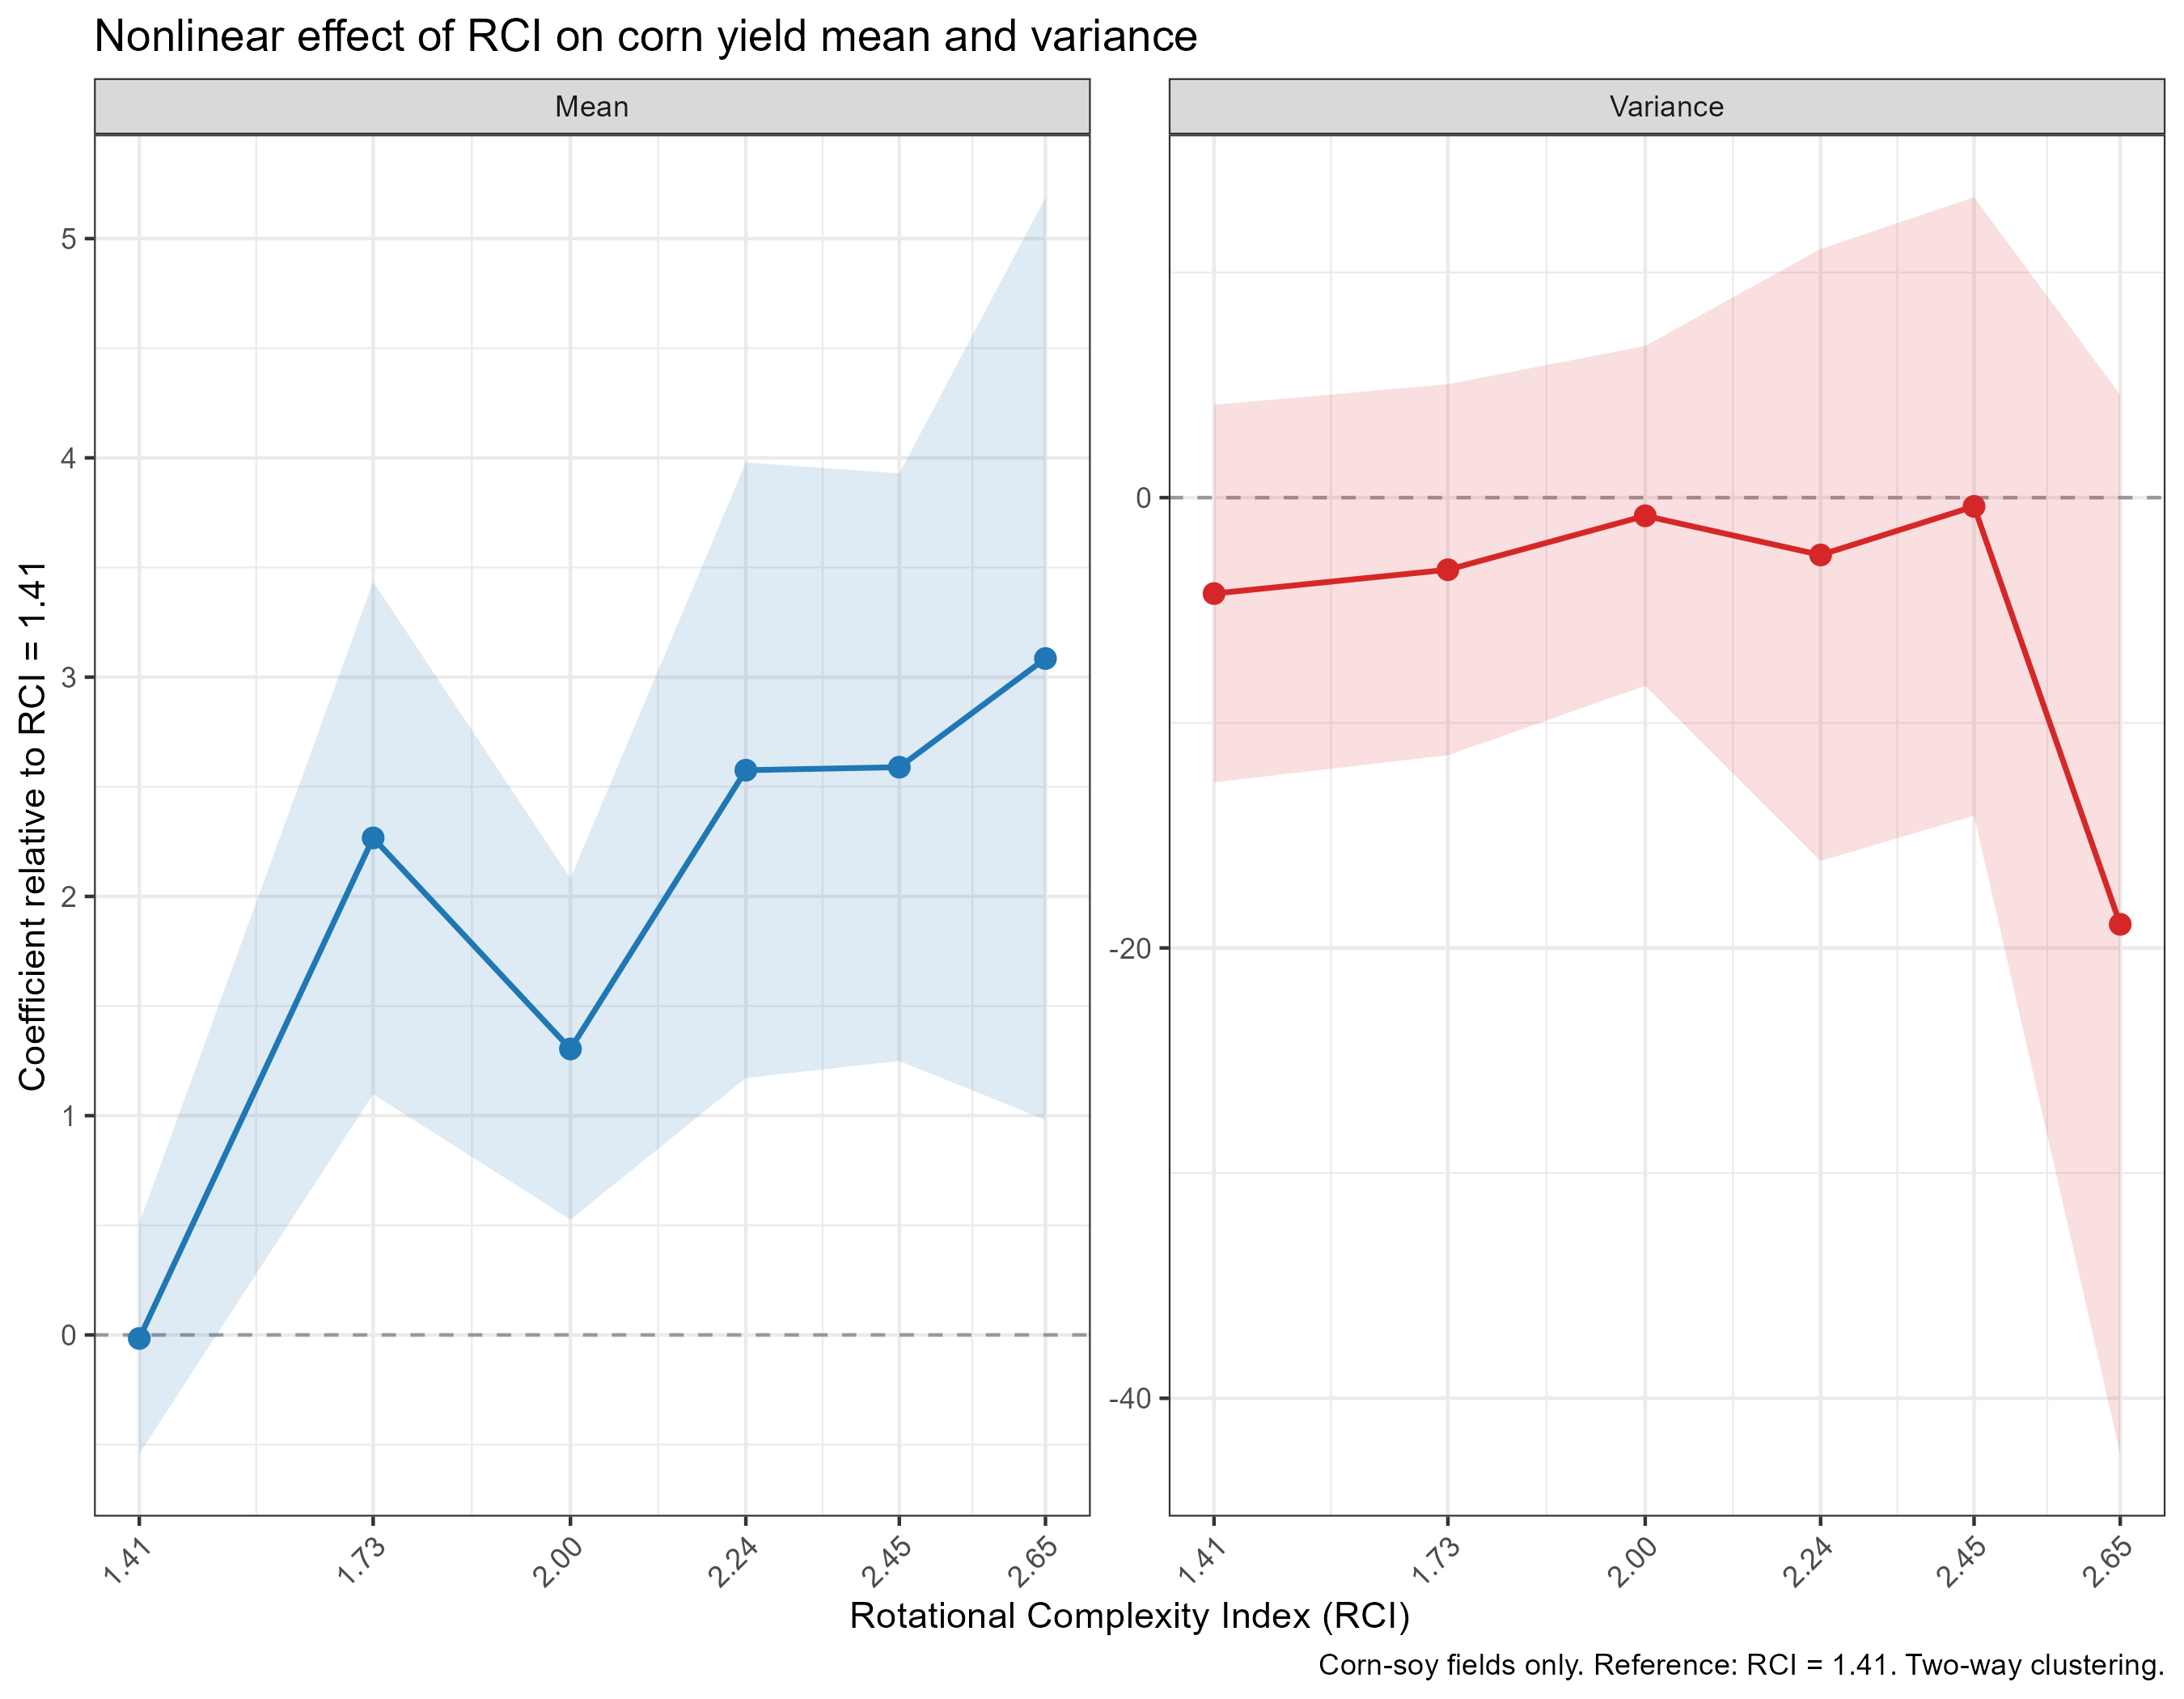
\includegraphics[width=\textwidth]{figures/rci_plot}
  \caption{Nonlinear effect of RCI on corn yield mean and variance.}
  \label{fig:rci_plot}
  \floatfoot{\footnotesize Notes: Factor RCI coefficients from
  equation~\eqref{eq:stage1} (mean, left panel) and equation~\eqref{eq:stage2}
  (variance, right panel). Shaded area is 95\% confidence interval. Reference:
  RCI = 1.41. Corn-soy fields only; two-way clustering at field and year level.}
\end{figure}

For soybean yields, the pattern is qualitatively similar but even flatter, with the highest RCI levels ($\geq 4.47$)
showing insignificant or negative coefficients.
 
\subsection{\label{subsec:rot_score_res}Rotation Score}

\begin{figure}[H]
  \centering
  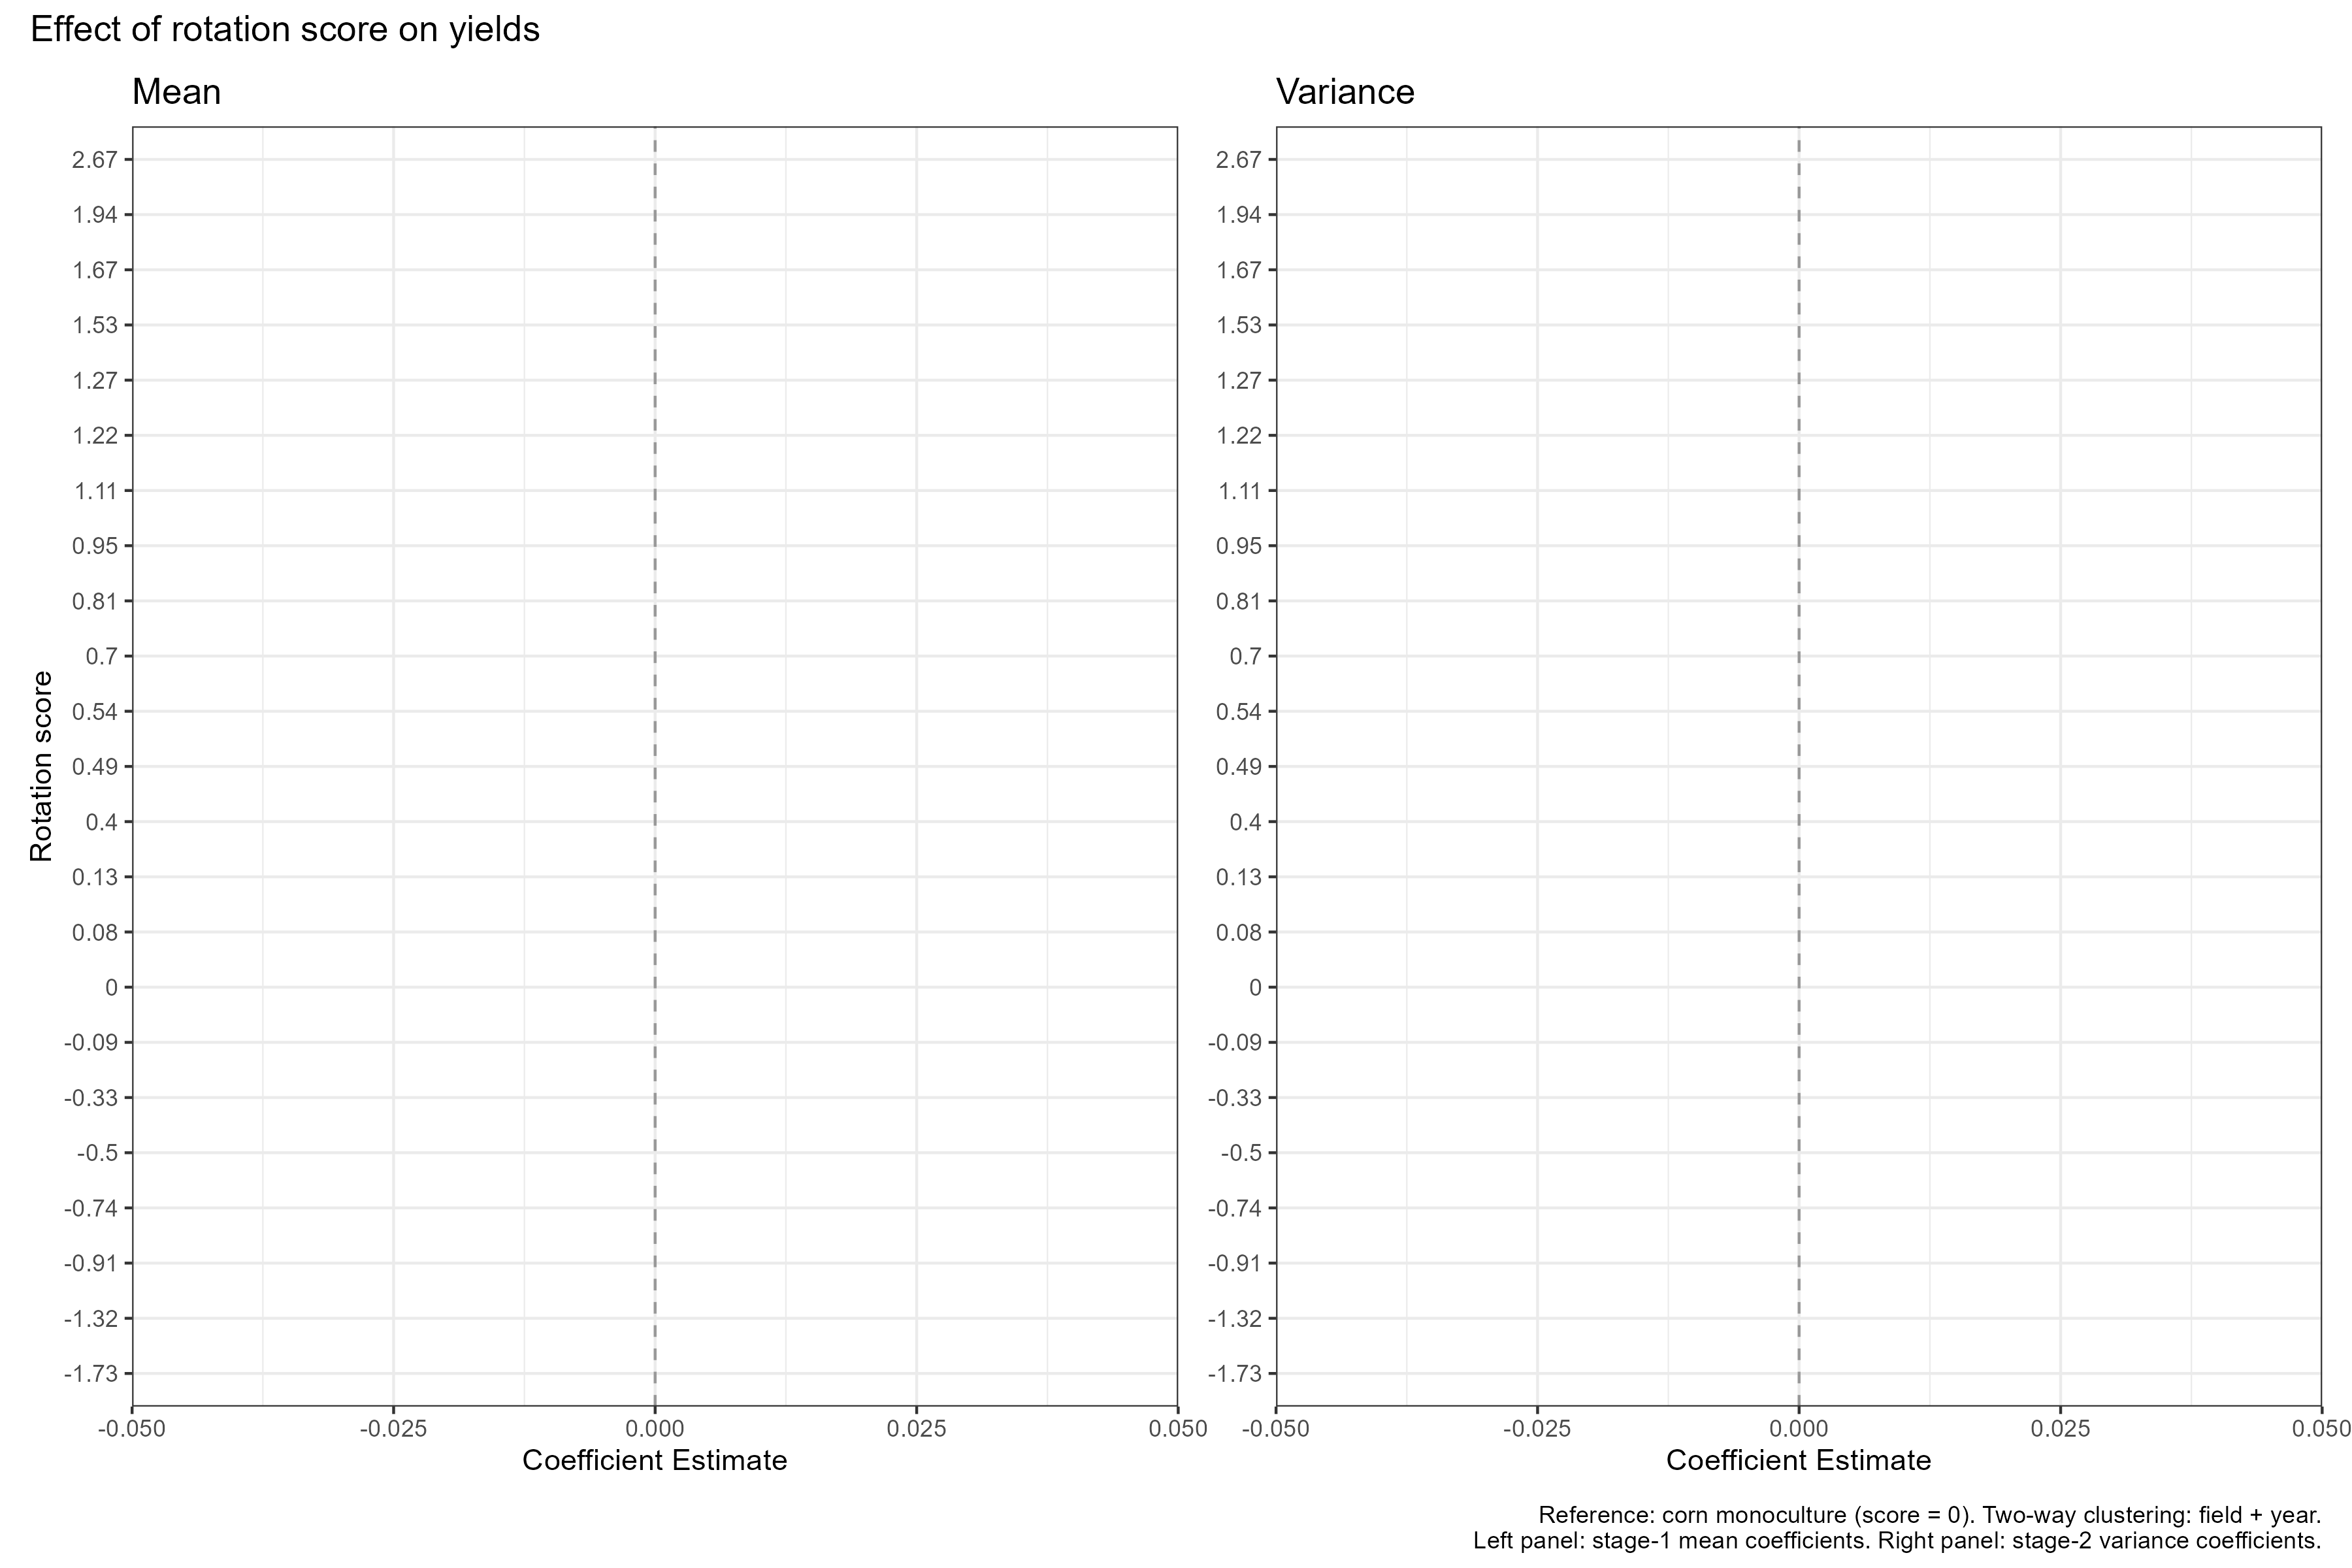
\includegraphics[width=\textwidth]{figures/score_yield}
  \caption{Response of corn yields to rotation score values.}
  \label{fig:score_yield}
  \floatfoot{\footnotesize Notes: Each row corresponds to one of the 14 distinct
  rotation score values, sorted in ascending order on the vertical axis. The
  rotation score is computed from equation~\eqref{eq:score} using the four
  Z-vector coefficients from Table~\ref{tab:zvector}: $\text{score}_{it} =
  \hat{\tau}_1 \cdot \text{late\_soy}_{it} + \hat{\tau}_2 \cdot
  \text{soy\_cons}_{it} + \hat{\tau}_3 \cdot \text{soy\_gap}_{it} +
  \hat{\tau}_4 \cdot n\text{soy}_{it}$. Left panel: stage-1 coefficient on mean
  corn yield (bushels per acre) from equation~\eqref{eq:stage1} with full
  rotation sequence indicators. Right panel: stage-2 OLS coefficient on
  conditional yield variance from equation~\eqref{eq:stage2}. Horizontal bars
  are 95\% confidence intervals. Reference: corn monoculture (score $= 0$).
  Two-way clustering at field and year level. Source: QDANN yield estimates,
  \citet{Ma2024}; CDL rotation histories, USDA-NASS.}
\end{figure}
 
Figure~\ref{fig:score_yield} reports predicted corn yields as a function of the rotation score. Score values range from approximately $-11.18$ (most soybean-heavy sequences with consecutive soybean years) to $+3.91$ (sequences with a very recent and optimally spaced soybean placement), with corn monoculture normalized to zero and the perfect alternating rotation scoring $+2.59$. The score-yield relationship is strongly positive and approximately linear across the upper portion of the score distribution (scores above $-2$). The score collapses 64 binary rotation sequences into 14 distinct score values, with variance effects showing a monotone negative relationship with score across most of the distribution.

\section{\label{sec:conclusions}Discussion and Conclusions} 
\subsection{\label{susec:summary}Summary of Findings}
 
This paper uses a large satellite-based field-level panel for Illinois from 2003 to 2022 to estimate how six-year crop rotation sequences affect both the mean and variance of corn and soybean yields. Our main findings are four.
 
First, the effect of crop rotation on corn yields depends critically on the timing and spacing of soybean placements within the six-year rotation window. A recent soybean harvest raises corn yields by approximately 2.85 to 3.55 bushels per acre per year of recency, while consecutive soybean years reduce yields by more than 4 bushels per acre relative to corn monoculture.
 
Second, the same structural features that raise mean yields also reduce yield variance. Sequences with recent, well-spaced soybean placements exhibit lower conditional yield variance than monoculture, while sequences with consecutive soybean years exhibit substantially higher variance. This joint mean-variance dominance implies that the best rotation sequences present unambiguously lower actuarial risk than monoculture at any given APH level.
 
Third, the RCI has a nonlinear and non-monotone relationship with corn yields that cannot be captured by a linear premium adjustment. The RCI effect flattens beyond RCI = 2.24 and provides no reliable signal for distinguishing the highest-risk sequences from one another.
 
Fourth, we develop a rotation score, constructed from four structural sequence features, that maps all 64 binary rotation sequences to 14 distinct values. The score summarizes the actuarially relevant information in the rotation history and is linearly related to yield outcomes across most of its support, making it suitable as a direct input to a rating formula.
 
\subsection{\label{subsec:implications}Implications for Crop Insurance Rating}
 
Our findings have direct implications for how rotation information could be incorporated into federal crop insurance rates. The rotation score provides a tractable rating instrument: a premium discount for fields with high rotation scores and a surcharge for fields with consecutive soybean years could be implemented within the existing APH framework by conditioning the base premium rate on the CDL-derived score, which is publicly available at the field level at no marginal cost to the insurer. Holding APH constant, a field with consecutive soybean years faces approximately 79 bushels-squared per acre-squared of additional conditional yield variance, which translates to a meaningful increase in expected indemnities under Revenue Protection.
 
Two challenges complicate straightforward implementation. First, the transition penalty we document implies that the APH would temporarily fall for fields moving from monoculture toward a corn-soy rotation, reducing the insurance guarantee precisely when farmers are bearing the costs of practice change, consistent with \citet{Connor2022}. A rotation-conditioned rate should handle this asymmetry explicitly, for example by using the score only after a minimum number of years in the target rotation. Second, the RCI nonlinearity documented here implies that blanket discounts for any field above a minimum RCI threshold would be poorly targeted. Any rating reform based on rotation history should incorporate sequence-level information of the kind the score captures.
 
\subsection{\label{subsec:limitations}Limitations and Future Work}
 
Several limitations warrant acknowledgment. First, our yield data come from
satellite-based estimators with meaningful field-level error rates. Measurement error in yields will tend to attenuate our rotation effect estimates toward zero, suggesting the true agronomic rotation premium may be larger than what we document.
 
Second, our identification strategy relies on within-county variation in rotation sequences across fields, which does not fully address the possibility that unobserved field-level characteristics drive both rotation choice and yield outcomes. Specifications with field fixed effects, explored as a robustness check, address this concern at the cost of restricting identification to fields that change rotation patterns over time.
 
Third, our analysis is restricted to Illinois corn-soy rotations. Generalizability to other Corn Belt states, to rotations involving a third crop, or to different climate and soil regimes is an open question. Finally, rotation decisions respond endogenously to prices and the proximity of grain market infrastructure such as ethanol refineries \citep{Pates2025,cheu2025}. A full welfare analysis of rotation-conditioned rates would require modeling the joint distribution of rotation choice and yield outcomes under the counterfactual rate schedule, which we leave for future work.

\section{\label{sec:conclusion}Conclusion}
 
Crop rotation history contains actuarially significant information about both the mean and variance of corn and soybean yields that the current APH-based rating system does not exploit. The key driver is not rotational complexity per se but the timing and spacing of soybean placements within the most recent six years. Fields with a recent, well-spaced soybean harvest present lower yield risk than monoculture fields at the same APH level; fields with consecutive soybean years present higher risk. These effects are large enough to be actuarially significant and are robust across two independent yield estimators. The rotation score we develop provides a tractable, publicly available, field-level rating variable. Identifying how this score should be translated into premium adjustments-and how the transition penalty should be handled for adopting farmers-are the key remaining design questions for rotation-conditioned federal crop insurance.

\newpage
\bibliography{bibliography.bib}

\newpage
\appendix

\section*{Tables}
 

\begin{table}[H]
   \caption{\label{tab:corn_rci_jp} Just-Pope: factor RCI and corn yield moments}
   \bigskip
   \centering
   \begin{tabular}{lcc}
      \toprule
                                      & corn\_yield          & resid\_sq\\   
                                      & Mean                 & Variance \\   
                                      & (1)                  & (2)\\  
      \midrule 
      RCI = 1.41                      & 0.1133 (1.278)       & -8.801 (10.23)\\   
      RCI = 1.73                      & -2.336 (1.590)       & 5.031 (17.63)\\   
      RCI = 2                         & -0.4267 (1.118)      & 1.148 (8.530)\\   
      RCI = 2.24                      & -0.5367 (1.376)      & 1.222 (8.965)\\   
      RCI = 2.45                      & -0.0163 (1.316)      & 4.833 (10.09)\\   
      RCI = 2.65                      & 0.7787 (1.371)       & -1.980 (9.868)\\   
      RCI = 2.74                      & 2.080 (1.744)        & -15.34 (15.15)\\   
      RCI = 3                         & -0.3399 (1.900)      & -30.51 (23.78)\\   
      RCI = 3.24                      & 1.538 (1.920)        & -36.69 (22.12)\\   
      RCI = 3.46                      & 3.957 (3.199)        & -44.62 (35.92)\\   
      RCI = 3.74                      & 3.764 (2.644)        & -64.85$^{*}$ (31.69)\\   
      RCI = 4                         & 7.918$^{**}$ (2.993) & -58.09 (38.90)\\   
       \\
      Observations                    & 1,640,455            & 1,640,455\\  
      R$^2$                           & 0.83737              & 0.30092\\  
      Within R$^2$                    & 0.13850              & 0.01313\\  
       \\
      tile\_field\_ID fixed effects   & $\checkmark$         & $\checkmark$\\   
      year fixed effects              & $\checkmark$         & $\checkmark$\\   
      \bottomrule
   \end{tabular}
\end{table}



\begin{quote}
\small
Notes: Column (1) reports stage-1 mean coefficients; column (2) reports stage-2 OLS variance coefficients. Reference: RCI = 1.41. Corn-soy fields only. Two-way clustering at field and year level.
\end{quote}
% TODO: verify reference category -- RCI = 1.41 appears in this table as its own row with an estimated coefficient, which is inconsistent with it being the omitted reference level. Confirm which RCI value is actually omitted.
 

\begin{table}[H]
   \caption{\label{tab:soy_rci_jp} Just-Pope: factor RCI and soy yield moments}
   \bigskip
   \centering
   \begin{tabular}{lcc}
      \toprule
                                      & soy\_yield              & resid\_sq\\   
                                      & Mean                    & Variance \\   
                                      & (1)                     & (2)\\  
      \midrule 
      RCI = 1.41                      & 0.6752$^{**}$ (0.2758)  & 0.0583 (1.764)\\   
      RCI = 1.73                      & 1.040$^{***}$ (0.2433)  & 0.4613 (1.446)\\   
      RCI = 2                         & 0.8345$^{***}$ (0.2590) & 0.4960 (1.458)\\   
      RCI = 2.24                      & 0.7112$^{**}$ (0.2895)  & 1.085 (1.529)\\   
      RCI = 2.45                      & 0.7952$^{**}$ (0.2703)  & 1.053 (1.557)\\   
      RCI = 2.74                      & 1.294$^{***}$ (0.3112)  & 0.2503 (1.990)\\   
      RCI = 3                         & 0.6524$^{**}$ (0.2422)  & 1.612 (1.875)\\   
      RCI = 3.24                      & 1.707$^{***}$ (0.4974)  & 0.8848 (2.137)\\   
      RCI = 3.46                      & 1.593$^{**}$ (0.6009)   & 1.188 (2.157)\\   
      RCI = 3.67                      & -0.1178 (0.8869)        & 2.233 (3.056)\\   
      RCI = 3.74                      & 1.423$^{*}$ (0.7018)    & 0.6083 (1.813)\\   
      RCI = 4                         & 2.955$^{***}$ (0.7634)  & -0.8129 (3.205)\\   
      RCI = 4.24                      & 0.3931 (0.9074)         & 2.500 (2.258)\\   
       \\
      Observations                    & 1,389,512               & 1,389,512\\  
      R$^2$                           & 0.80535                 & 0.31965\\  
      Within R$^2$                    & 0.08001                 & 0.00452\\  
       \\
      tile\_field\_ID fixed effects   & $\checkmark$            & $\checkmark$\\   
      year fixed effects              & $\checkmark$            & $\checkmark$\\   
      \bottomrule
   \end{tabular}
\end{table}



\begin{quote}
\small
Notes: See Table~\ref{tab:corn_rci_jp} notes. Dependent variable is soybean yield.
\end{quote}
 
%\begin{table}[H]
%  \centering
  %\caption{Effect of weather (VPD) and rotation sequences on corn yields}
  %\label{tab:rot_vpd}
%  \begin{threeparttable}
%  \scriptsize
%    
\begin{table}[htbp]
   \caption{\label{tab:rot_vpd} Effect of weather and rotation sequences on corn and soybean yields}
   \bigskip
   \centering
   \begin{tabular}{lcccc}
      \toprule
       & \multicolumn{2}{c}{corn\_yield} & \multicolumn{2}{c}{soy\_yield}\\
      Corn yields & \multicolumn{4}{c}{2} \\ 
      Soy yields & \multicolumn{4}{c}{2} \\ 
                                      & (1)            & (2)            & (3)            & (4)\\  
      \midrule 
      C-C-C-C-S-C                     & 4.040$^{***}$  & 3.819$^{***}$  &                &   \\   
                                      & (0.3515)       & (0.3373)       &                &   \\   
      C-C-C-S-C-C                     & 2.247$^{***}$  & 1.792$^{***}$  &                &   \\   
                                      & (0.2496)       & (0.2385)       &                &   \\   
      C-C-C-S-S-C                     & 3.038$^{***}$  & 3.167$^{***}$  &                &   \\   
                                      & (0.5843)       & (0.5097)       &                &   \\   
      C-C-S-C-C-C                     & 0.9367$^{***}$ & 0.6261$^{**}$  &                &   \\   
                                      & (0.3102)       & (0.2734)       &                &   \\   
      C-C-S-C-S-C                     & 3.431$^{***}$  & 3.257$^{***}$  &                &   \\   
                                      & (0.4843)       & (0.3985)       &                &   \\   
      C-C-S-S-C-C                     & -0.2788        & -0.2209        &                &   \\   
                                      & (0.8249)       & (0.7571)       &                &   \\   
      C-C-S-S-S-C                     & 2.037$^{***}$  & 2.329$^{***}$  &                &   \\   
                                      & (0.7160)       & (0.6309)       &                &   \\   
      C-S-C-C-C-C                     & -0.3984        & -0.3644        &                &   \\   
                                      & (0.3555)       & (0.2747)       &                &   \\   
      C-S-C-C-S-C                     & 3.568$^{***}$  & 3.208$^{***}$  &                &   \\   
                                      & (0.4639)       & (0.3822)       &                &   \\   
      C-S-C-S-C-C                     & 1.429$^{***}$  & 1.024$^{***}$  &                &   \\   
                                      & (0.4546)       & (0.3864)       &                &   \\   
      C-S-C-S-S-C                     & 4.531$^{***}$  & 3.825$^{***}$  &                &   \\   
                                      & (0.5874)       & (0.4767)       &                &   \\   
      C-S-S-C-C-C                     & 0.5190         & 0.8892         &                &   \\   
                                      & (0.8784)       & (0.7955)       &                &   \\   
      C-S-S-C-S-C                     & 1.800$^{**}$   & 1.770$^{***}$  &                &   \\   
                                      & (0.7946)       & (0.6065)       &                &   \\   
      C-S-S-S-C-C                     & -1.147         & -0.8615        &                &   \\   
                                      & (1.142)        & (0.9941)       &                &   \\   
      C-S-S-S-S-C                     & 3.794$^{***}$  & 3.653$^{***}$  &                &   \\   
                                      & (0.7355)       & (0.6326)       &                &   \\   
      S-C-C-C-C-C                     & -0.3701        & -0.5853$^{**}$ &                &   \\   
                                      & (0.2981)       & (0.2432)       &                &   \\   
      S-C-C-C-S-C                     & 4.172$^{***}$  & 3.630$^{***}$  &                &   \\   
                                      & (0.4407)       & (0.3728)       &                &   \\   
      S-C-C-S-C-C                     & 1.680$^{***}$  & 1.167$^{***}$  &                &   \\   
                                      & (0.4067)       & (0.3576)       &                &   \\   
      S-C-C-S-S-C                     & 3.514$^{***}$  & 2.800$^{***}$  &                &   \\   
                                      & (0.7671)       & (0.6293)       &                &   \\   
      S-C-S-C-C-C                     & 1.208$^{***}$  & 0.8390$^{**}$  &                &   \\   
                                      & (0.4149)       & (0.3552)       &                &   \\   
      S-C-S-C-S-C                     & 3.510$^{***}$  & 2.891$^{***}$  &                &   \\   
                                      & (0.5408)       & (0.4164)       &                &   \\   
      S-C-S-S-C-C                     & 0.5262         & 0.0183         &                &   \\   
                                      & (0.6882)       & (0.6031)       &                &   \\   
      S-C-S-S-S-C                     & 4.517$^{***}$  & 3.695$^{***}$  &                &   \\   
                                      & (0.6716)       & (0.5534)       &                &   \\   
      S-S-C-C-C-C                     & 0.4403         & 0.2164         &                &   \\   
                                      & (0.7483)       & (0.6703)       &                &   \\   
      S-S-C-C-S-C                     & 4.155$^{***}$  & 3.373$^{***}$  &                &   \\   
                                      & (0.7076)       & (0.6052)       &                &   \\   
      S-S-C-S-C-C                     & 0.6781         & -0.2150        &                &   \\   
                                      & (0.7048)       & (0.5685)       &                &   \\   
      S-S-C-S-S-C                     & 6.094$^{***}$  & 4.795$^{***}$  &                &   \\   
                                      & (0.6948)       & (0.6313)       &                &   \\   
      S-S-S-C-C-C                     & 0.3203         & 0.1237         &                &   \\   
                                      & (1.101)        & (0.8973)       &                &   \\   
      S-S-S-C-S-C                     & 2.742$^{***}$  & 2.412$^{***}$  &                &   \\   
                                      & (0.7768)       & (0.6017)       &                &   \\   
      S-S-S-S-C-C                     & 2.629$^{**}$   & 1.492          &                &   \\   
                                      & (1.239)        & (1.165)        &                &   \\   
      S-S-S-S-S-C                     & 4.028$^{***}$  & 3.525$^{***}$  &                &   \\   
                                      & (0.8932)       & (0.7455)       &                &   \\   
      Somewhat dry season             & -2.353$^{***}$ & -1.380$^{**}$  & -0.2853        & -0.4989$^{***}$\\   
                                      & (0.5499)       & (0.6260)       & (0.1932)       & (0.1535)\\   
      Dry season                      & -6.267$^{***}$ & -2.892$^{***}$ & -0.2134        & -0.4391$^{**}$\\   
                                      & (0.8381)       & (0.7835)       & (0.2673)       & (0.2118)\\   
      C-C-C-C-C-S                     &                &                & 1.450$^{***}$  & 1.671$^{***}$\\   
                                      &                &                & (0.2004)       & (0.1722)\\   
      C-C-C-C-S-S                     &                &                & 0.6123$^{***}$ & 0.9274$^{***}$\\   
                                      &                &                & (0.2088)       & (0.1820)\\   
      C-C-C-S-C-S                     &                &                & 0.9515$^{***}$ & 1.207$^{***}$\\   
                                      &                &                & (0.1635)       & (0.1564)\\   
      C-C-C-S-S-S                     &                &                & 0.2559         & 0.4533$^{**}$\\   
                                      &                &                & (0.2263)       & (0.2207)\\   
      C-C-S-C-C-S                     &                &                & 0.9409$^{***}$ & 1.262$^{***}$\\   
                                      &                &                & (0.1650)       & (0.1567)\\   
      C-C-S-C-S-S                     &                &                & 0.1286         & 0.4816$^{***}$\\   
                                      &                &                & (0.1794)       & (0.1767)\\   
      C-C-S-S-C-S                     &                &                & 0.3329$^{**}$  & 0.6522$^{***}$\\   
                                      &                &                & (0.1583)       & (0.1509)\\   
      C-C-S-S-S-S                     &                &                & -0.1266        & 0.1919\\   
                                      &                &                & (0.2185)       & (0.2171)\\   
      C-S-C-C-C-S                     &                &                & 0.9748$^{***}$ & 1.284$^{***}$\\   
                                      &                &                & (0.1576)       & (0.1518)\\   
      C-S-C-C-S-S                     &                &                & -0.1955        & 0.1594\\   
                                      &                &                & (0.1758)       & (0.1680)\\   
      C-S-C-S-C-S                     &                &                & 0.5736$^{***}$ & 0.8748$^{***}$\\   
                                      &                &                & (0.1353)       & (0.1414)\\   
      C-S-C-S-S-S                     &                &                & 0.1025         & 0.2663$^{*}$\\   
                                      &                &                & (0.1317)       & (0.1359)\\   
      C-S-S-C-C-S                     &                &                & 0.9700$^{***}$ & 1.257$^{***}$\\   
                                      &                &                & (0.1742)       & (0.1718)\\   
      C-S-S-C-S-S                     &                &                & 0.1788         & 0.3156$^{***}$\\   
                                      &                &                & (0.1151)       & (0.1196)\\   
      C-S-S-S-C-S                     &                &                & 0.3884$^{***}$ & 0.6859$^{***}$\\   
                                      &                &                & (0.1294)       & (0.1278)\\   
      C-S-S-S-S-S                     &                &                & -0.0278        & 0.0644\\   
                                      &                &                & (0.0965)       & (0.0874)\\   
      S-C-C-C-C-S                     &                &                & 1.290$^{***}$  & 1.425$^{***}$\\   
                                      &                &                & (0.1879)       & (0.1670)\\   
      S-C-C-C-S-S                     &                &                & 0.4058$^{*}$   & 0.6665$^{***}$\\   
                                      &                &                & (0.2249)       & (0.2128)\\   
      S-C-C-S-C-S                     &                &                & 0.8435$^{***}$ & 1.101$^{***}$\\   
                                      &                &                & (0.1394)       & (0.1428)\\   
      S-C-C-S-S-S                     &                &                & -0.0058        & 0.3291$^{*}$\\   
                                      &                &                & (0.2094)       & (0.1820)\\   
      S-C-S-C-C-S                     &                &                & 0.9584$^{***}$ & 1.232$^{***}$\\   
                                      &                &                & (0.1437)       & (0.1466)\\   
      S-C-S-C-S-S                     &                &                & 0.0525         & 0.3343$^{**}$\\   
                                      &                &                & (0.1281)       & (0.1274)\\   
      S-C-S-S-C-S                     &                &                & 0.2893$^{**}$  & 0.6014$^{***}$\\   
                                      &                &                & (0.1195)       & (0.1290)\\   
      S-C-S-S-S-S                     &                &                & -0.1974$^{**}$ & 0.0059\\   
                                      &                &                & (0.0865)       & (0.0948)\\   
      S-S-C-C-C-S                     &                &                & 0.9200$^{***}$ & 1.013$^{***}$\\   
                                      &                &                & (0.2556)       & (0.2370)\\   
      S-S-C-C-S-S                     &                &                & -0.0649        & 0.0471\\   
                                      &                &                & (0.2709)       & (0.2669)\\   
      S-S-C-S-C-S                     &                &                & 0.4987$^{***}$ & 0.6444$^{***}$\\   
                                      &                &                & (0.1296)       & (0.1389)\\   
      S-S-C-S-S-S                     &                &                & 0.0028         & 0.0208\\   
                                      &                &                & (0.1169)       & (0.1132)\\   
      S-S-S-C-C-S                     &                &                & 1.319$^{***}$  & 1.496$^{***}$\\   
                                      &                &                & (0.2268)       & (0.2181)\\   
      S-S-S-C-S-S                     &                &                & 0.2335$^{**}$  & 0.2338$^{**}$\\   
                                      &                &                & (0.0942)       & (0.0906)\\   
      S-S-S-S-C-S                     &                &                & 0.5007$^{***}$ & 0.6605$^{***}$\\   
                                      &                &                & (0.1030)       & (0.1127)\\   
       \\
      Observations                    & 1,538,965      & 1,538,965      & 1,328,023      & 1,328,023\\  
      R$^2$                           & 0.83510        & 0.86195        & 0.79129        & 0.80945\\  
      Within R$^2$                    & 0.01339        & 0.17402        & 0.00301        & 0.08976\\  
      Controls                        & No             & Yes            & No             & Yes\\  
       \\
      tile\_field\_ID fixed effects   & $\checkmark$   & $\checkmark$   & $\checkmark$   & $\checkmark$\\   
      year fixed effects              & $\checkmark$   & $\checkmark$   & $\checkmark$   & $\checkmark$\\   
      \bottomrule
   \end{tabular}
\end{table}



%    \begin{tablenotes}
%      \small
%      \item Notes: Dependent variables are QDANN corn yield (columns 1-2) and
%      QDANN soybean yield (columns 3-4) in bushels per acre. VPD bins defined
%      as: normal ($<$1.9 kPa), somewhat dry (1.9-2.1 kPa), dry ($>$2.1 kPa),
%      measured in July. Reference: normal VPD, corn monoculture (columns 1-2)
%      or soy monoculture (columns 3–4). Standard errors in parentheses, two-way
%      clustered at field and year level.
%      $^{***}p<0.01$, $^{**}p<0.05$, $^{*}p<0.10$.
%    \end{tablenotes}
%  \end{threeparttable}
%\end{table}
 
 
\clearpage
\section*{Figures}
 
\begin{figure}[H]
  \centering
  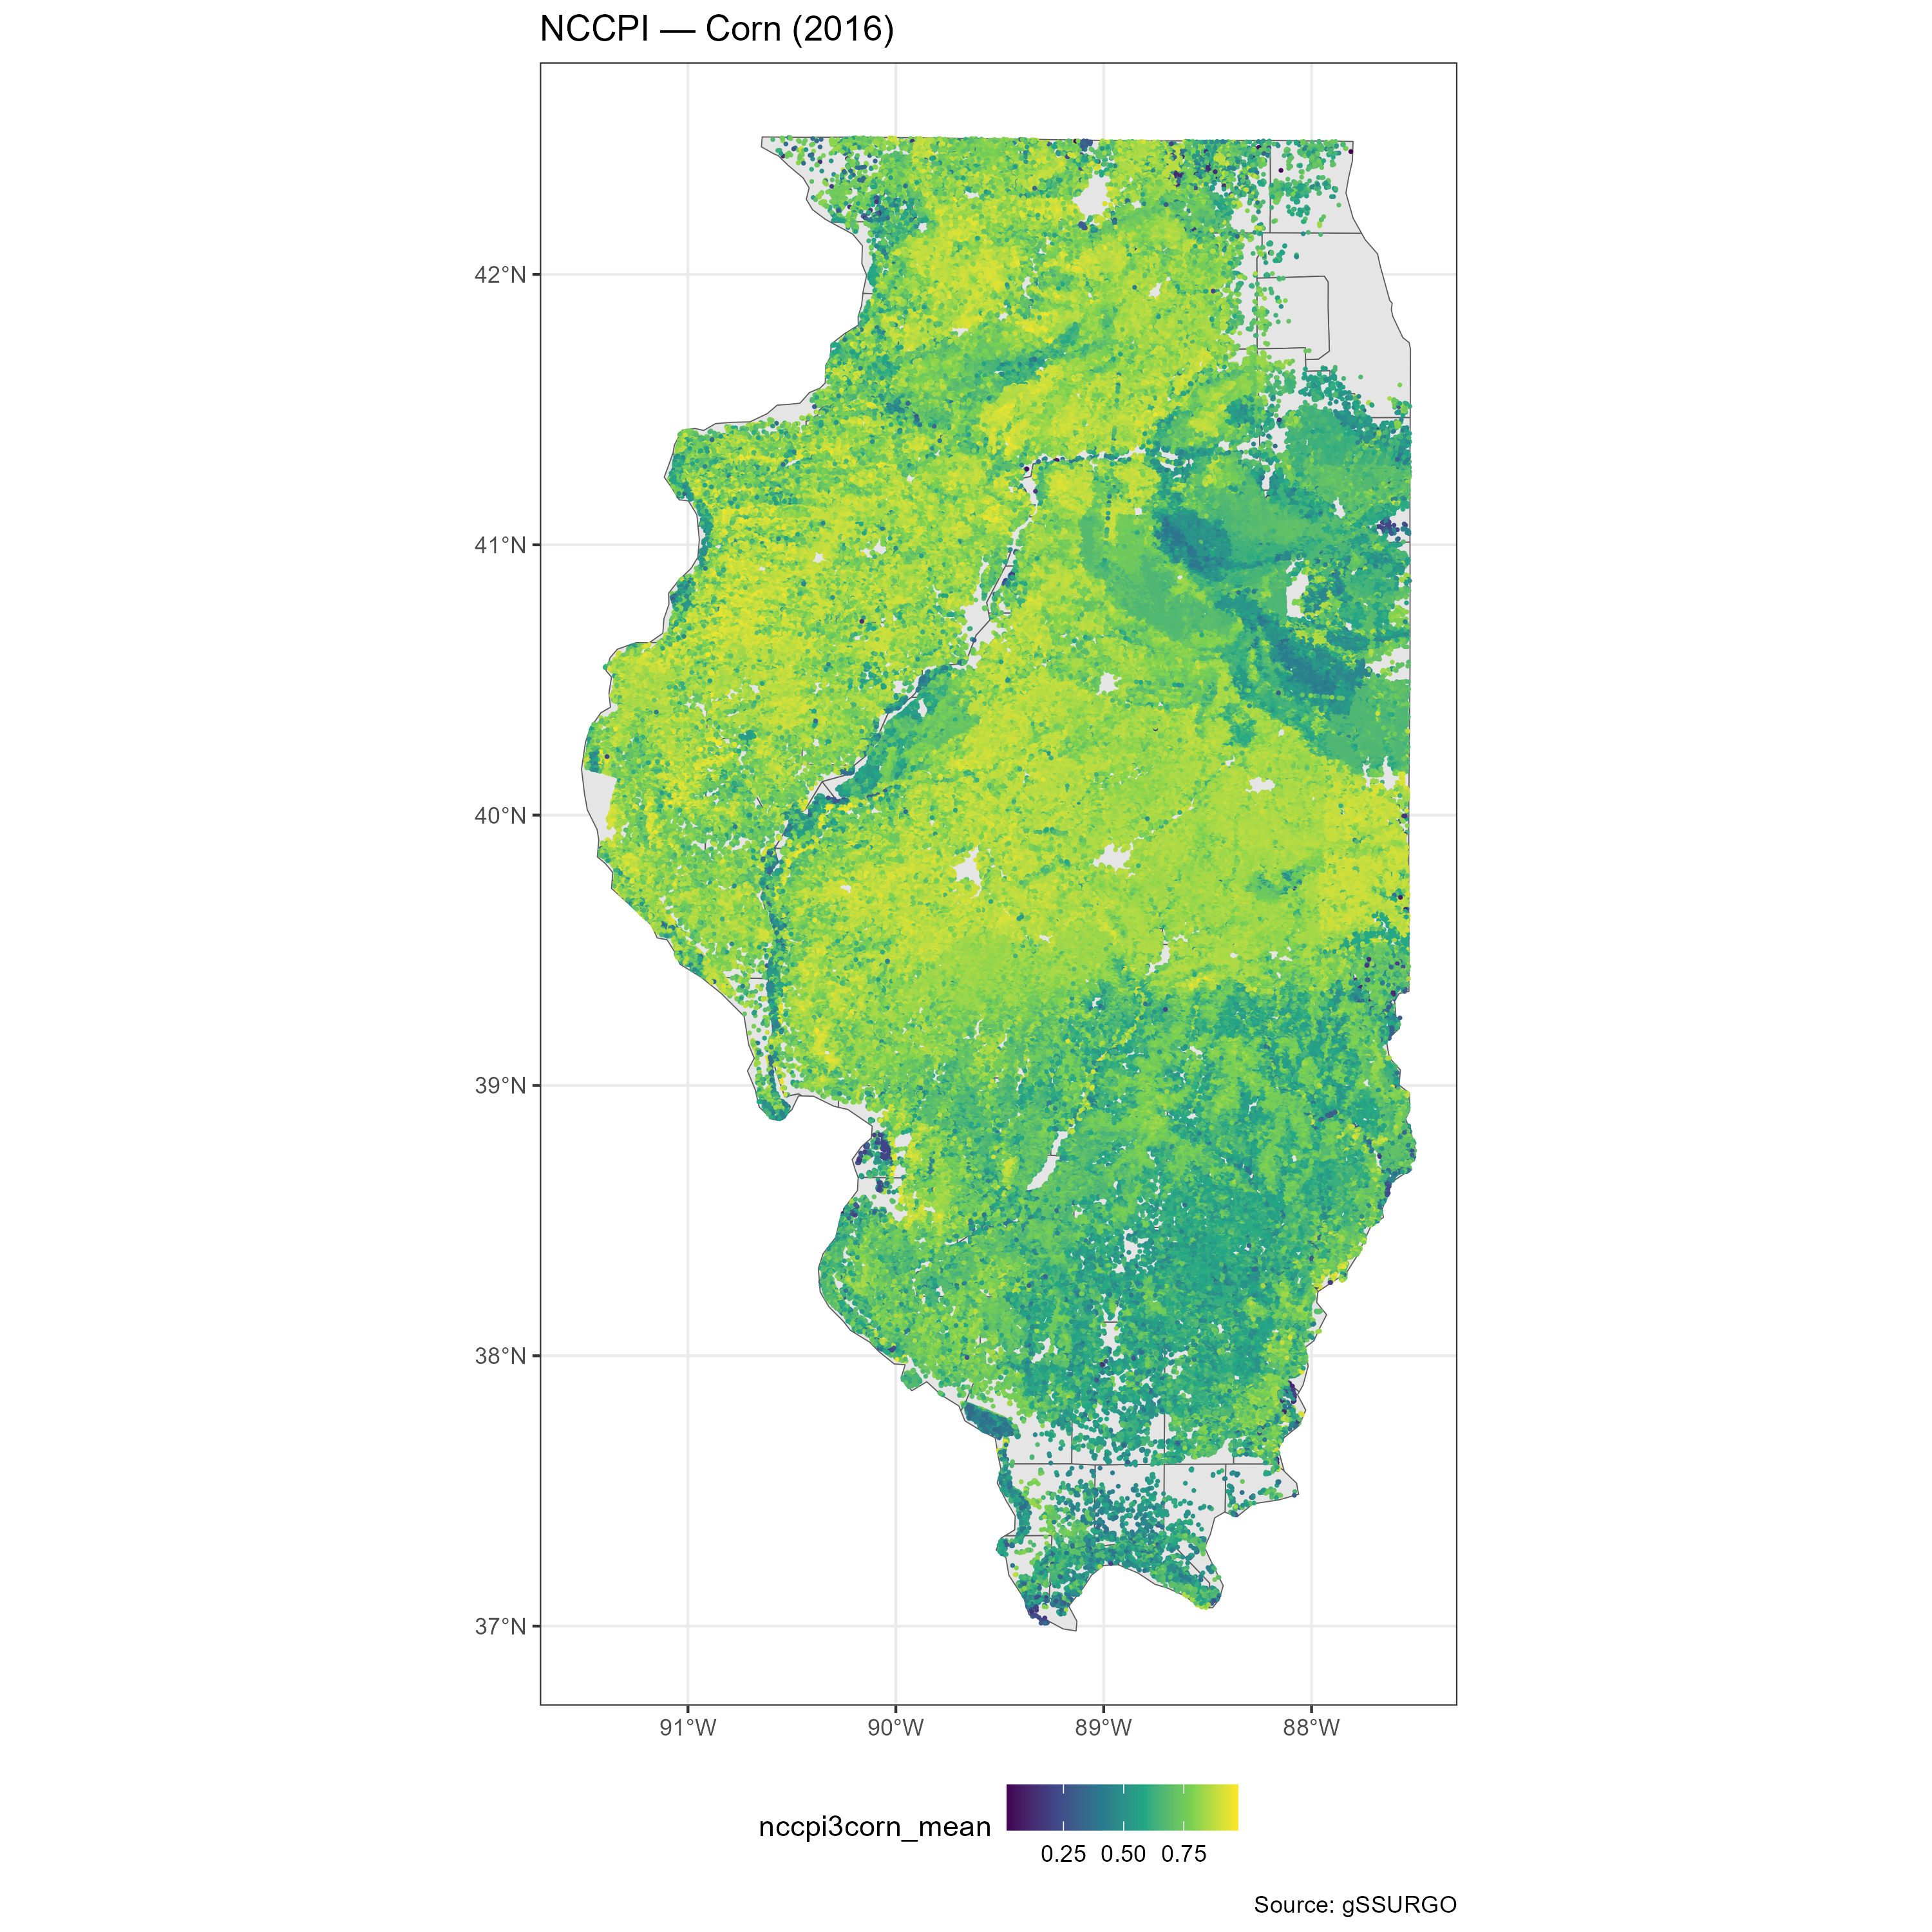
\includegraphics[width=0.85\textwidth]{figures/nccpi_corn_map}
  \caption{National Commodity Crop Productivity Index (corn) across Illinois.}
  \label{fig:nccpi_corn_map}
  \floatfoot{\footnotesize Notes: NCCPI corn values at 30-meter resolution.
  Source: gSSURGO, USDA-NRCS.}
\end{figure}
	
\end{document}